\documentclass[12pt, uplatex]{jsbook}

%%%%%%%%%%%%%%%%%%%%%%%%%%%%%%%%%%%%%%%%%%%%%%%%%%%%%%%%%%%%%%%%%%%%%%%%%%%%%%%
%%%%%%%%%%%%%%%%%%%%%%%%%%%%%%%%%%%%%%%%%%%%%%%%%%%%%%%%%%%%%%%%%%%%%%%%%%%%%%%
%
%   Define.tex
%   ==========
%
%
%%%%%%%%%%%%%%%%%%%%%%%%%%%%%%%%%%%%%%%%%%%%%%%%%%%%%%%%%%%%%%%%%%%%%%%%%%%%%%%
%%%%%%%%%%%%%%%%%%%%%%%%%%%%%%%%%%%%%%%%%%%%%%%%%%%%%%%%%%%%%%%%%%%%%%%%%%%%%%%
%\input{epsf.sty}    %   To input figure

\usepackage{amsmath,amssymb,color,latexSym, mathrsfs}
%\usepackage{epsfig,tabularx,a4wide,amsmath,amsSymb,color,latexSym,pifont,epsf,txfonts,mathrsfs,yfonts}
%\usepackage[sf,bf,compact,topmarks,calcwidth,pagestyles]{titlesec}
%\usepackage{titletoc}
%\usepackage{bbm}
%\usepackage[OMLmathrm,OMLmathbf]{isomath}
\DeclareMathAlphabet{\mathbbmsl}{U}{bbm}{m}{sl}
%\textheight 23cm \textwidth 16.5cm \topmargin 0pt \hoffset 0pt
%\oddsidemargin 0pt \voffset 0pt \headheight 0pt \headsep 0pt
%\marginparwidth 0pt \sloppypar \flushbottom
%
\def\LargeFS{8cm}
\def\OneFS{6cm}
\def\TwoFS{4cm}
\def\SmallFS{3cm}
\def\TinyFS{2cm}
%
\def\BE{\begin{eqnarray}}
\def\NN{\nonumber}
\def\EE{\end{eqnarray}}
\def\BM{\begin{bmatrix}}
\def\EM{\end{bmatrix}}
\def\BI{\begin{itemize}}
\def\EI{\end{itemize}}
\def\BC{\begin{center}}
\def\EC{\end{center}}
\def\BNUM{\begin{enumerate}}
\def\ENUM{\end{enumerate}}
%

%
\def\A{\mbox{\boldmath$A$}}
\def\B{\mbox{\boldmath$B$}}
\def\C{\mbox{\boldmath$C$}}
\def\D{\mbox{\boldmath$D$}}
\def\E{\mbox{\boldmath$E$}}
\def\F{\mbox{\boldmath$F$}}
\def\G{\mbox{\boldmath$G$}}
\def\HH{\mbox{\boldmath$H$}}
\def\I{\mbox{\boldmath$I$}}
\def\J{\mbox{\boldmath$J$}}
\def\K{\mbox{\boldmath$K$}}

\def\LL{{\boldmath$L$}}
\def\M{\mbox{\boldmath$M$}}
\def\N{\mbox{\boldmath$N$}}
\def\OO{\mbox{\boldmath$O$}}
\def\P{\mbox{\boldmath$P$}}
\def\Q{\mbox{\boldmath$Q$}}
\def\R{\mbox{\boldmath$R$}}
\def\SS{{\boldmath{S}}}
\def\Ss{{\boldmath{S}}}
\def\T{\mbox{\boldmath$T$}}
\def\V{\mbox{\boldmath$V$}}
\def\W{\mbox{\boldmath$W$}}
\def\Y{\mbox{\boldmath$Y$}}
\def\Z{\mbox{\boldmath$Z$}}
%
\def\aa{\mbox{\boldmath$a$}}
\def\bb{\mbox{\boldmath$b$}}
\def\cc{\mbox{\boldmath$c$}}
\def\dd{\mbox{\boldmath$d$}}
\def\ee{\mbox{\boldmath$e$}}
\def\ff{\mbox{\boldmath$f$}}
\def\gg{\mbox{\boldmath$g$}}
\def\hh{\mbox{\boldmath$h$}}
\def\ii{\mbox{\boldmath$i$}}
\def\jj{\mbox{\boldmath$j$}}
\def\kk{\mbox{\boldmath$k$}}
\def\ll{\mbox{\boldmath$l$}}
\def\mm{\mbox{\boldmath$m$}}
\def\nn{\mbox{\boldmath$n$}}
\def\oo{\mbox{\boldmath$o$}}
\def\pp{\mbox{\boldmath$p$}}
\def\qq{\mbox{\boldmath$q$}}
\def\rr{\mbox{\boldmath$r$}}
\def\ss{\mbox{\boldmath$s$}}
\def\tt{\mbox{\boldmath$t$}}
\def\uu{\mbox{\boldmath$u$}}
\def\vv{\mbox{\boldmath$v$}}
\def\ww{\mbox{\boldmath$w$}}
\def\yy{\mbox{\boldmath$y$}}
\def\zz{\mbox{\boldmath$z$}}
%
%----------------------------------------------------------------
%       All x States
%----------------------------------------------------------------
\def\xAll{\mathbbmsl{x}}
\def\xAllMinus{\mathbbmsl{x}^{-}}
\def\xAllPlusPre{\mathbbmsl{x}^{+}_{t-1}}
\def\xAllPre{\mathbbmsl{x}_{t-1}}

%
%
\def\xAllHat{\hat{\mathbbmsl{x}}}
\def\xAllHatPlus{\hat{\mathbbmsl{x}}^{+}}
\def\xAllHatPlusPre{\hat{\mathbbmsl{x}}^{+}_{t-1}}
\def\xAllHatMinus{\hat{\mathbbmsl{x}}^{~-}}
%
\def\xAllTilde{\tilde{\mathbbmsl{x}}}
\def\xAllTildePlus{\tilde{\mathbbmsl{x}}^+}
\def\xAllTildePlusPre{\tilde{\mathbbmsl{x}}^+_{t-1}}
\def\xAllTildeMinus{\tilde{\mathbbmsl{x}}^-}
%
\def\xAllBar{\bar{\mathbbmsl{x}}}
\def\xAllBarPlus{\bar{\mathbbmsl{x}}^+}
\def\xAllBarMinus{\bar{\mathbbmsl{x}}^-}

\def\yAll{\mathbbmsl{y}}
\def\zAll{\mathbbmsl{z}}
\def\uAll{\mathbbmsl{u}}
\def\lAlll{\mathbbmsl{l}}
\def\MAll{\mathbbmsl{M}}
\def\sAll{\mathbbmsl{s}}
%
%
%----------------------------------------------------------------
%       vector x
%----------------------------------------------------------------
%
\def\x{\mbox{\boldmath$x$}}
\def\xx{\mbox{\boldmath$x$}}

%
\def\xR{\mbox{\boldmath{$x$}}_r}
\def\xRPre{\mbox{\boldmath{$x$}}_{r,t-1}}
\def\xMinusR{\mbox{\boldmath{$x$}}^-_r}
\def\xPlusR{\mbox{\boldmath{$x$}}^+_r}
\def\xPlusRPre{\mbox{\boldmath$x$}^+_{r,t-1}}
%
\def\RPrexR{(^{r,t-1}\mbox{\boldmath{$x$}}_{r})}
\def\RPrexHatR{(^{r,t-1}\hat{\mbox{\boldmath{$x$}}}_{r})}
\def\RPrexBarR{(^{r,t-1}\bar{\mbox{\boldmath{$x$}}}_{r})}
\def\RPrexTildeR{(^{r,t-1}\tilde{\mbox{\boldmath{$x$}}}_{r})}
\def\RPreDeltaxTildeR{(^{r,t-1}\widetilde{\delta \mbox{\boldmath{$x$}}}_{r})}
%
\def\xHat{\hat{\mbox{\boldmath{$x$}}}}
\def\xHatR{\hat{\mbox{\boldmath{$x$}}}_r}
\def\xHatRPre{\hat{\mbox{\boldmath{$x$}}}_{r,t-1}}
\def\xHatPlusR{\hat{\mbox{\boldmath$x$}}^+_{r}}
\def\xHatPlusRZero{\hat{\mbox{\boldmath$x$}}^+_{r,0}}
\def\xHatPlusRPre{\hat{\mbox{\boldmath$x$}}^+_{r,t-1}}
\def\xHatMinusR{\hat{\mbox{\boldmath$x$}}^-_{r}}
%
\def\xTilde{\tilde{\mbox{\boldmath{$x$}}}}
\def\xTildeR{\tilde{\mbox{\boldmath{$x$}}}_r}
\def\xTildeRPre{\tilde{\mbox{\boldmath{$x$}}}_{r,t-1}}
\def\xTildePlusR{\tilde{\mbox{\boldmath$x$}}^+_r}
\def\xTildePlusRPre{\tilde{\mbox{\boldmath$x$}}^+_{r,t-1}}
\def\xTildeMinusR{\tilde{\mbox{\boldmath$x$}}^-_{r}}
%
\def\xBar{\bar{\mbox{\boldmath{$x$}}}}
\def\xBarR{\bar{\mbox{\boldmath{$x$}}}_r}
\def\xBarPlusR{\bar{\mbox{\boldmath$x$}}^+_r}
\def\xBarPlusRPre{\bar{\mbox{\boldmath$x$}}^+_{r,t-1}}
\def\xBarMinusR{\bar{\mbox{\boldmath$x$}}^+_{r}}
%
\def\RxHatI{^r \hat{\mbox{\boldmath{$x$}}}_{i}}
\def\RxHatMinusW{^r \hat{\mbox{\boldmath{$x$}}}^-_{w}}
\def\RPrexHatMinusW{(^{r,t-1}\hat{\mbox{\boldmath{$x$}}}^{-}_{w})}
%\RPrexHatMinusW
%%----------------------------------------------------------------
%%       vector X
%%----------------------------------------------------------------
%%
\def\X{\mbox{\boldmath$X$}}
\def\XBar{\overline{\mbox{\boldmath{$X$}}}}
%
%
%----------------------------------------------------------------
%       scalar x: robot
%----------------------------------------------------------------
%
\def\Sx{x}
\def\SxR{x_r}
\def\SxPlusRPre{x^+_{r,t-1}}
%
\def\RPreSxR{(^{r,t-1} x_{r})}
\def\RPreDeltaSxR{(^{r,t-1} \delta x_{r})}
\def\RPreSxHatR{(^{r,t-1} \hat{x}_{r})}
\def\SxHatR{\hat{x}_r}
\def\SxHatRPre{\hat{x}_{r,t-1}}
\def\SxHatPlusR{\hat{x}^+_r}
\def\SxHatPlusRPre{\hat{x}^+_{r,t-1}}
\def\SxHatMinusR{\hat{x}^-_r}
\def\SxHatMinusI{\hat{x}^-_i}
\def\SxBar{\bar{x}}
%
\def\SxMinusR{x^-_{r}}
%----------------------------------------------------------------
%       vector y
%----------------------------------------------------------------
%
\def\y{\mbox{\boldmath$y$}}
%
%----------------------------------------------------------------
%       scalar y: robot
%----------------------------------------------------------------
%
\def\Sy{y}
\def\SyR{y_r}
\def\SyPlusRPre{y^+_{r,t-1}}
%
\def\SyRPre{y_{r,t-1}}
\def\RPreSyR{(^{r,t-1} y_{r})}
\def\RPreSyHatR{(^{r,t-1} \hat{y}_{r})}
\def\RPreDeltaSyR{(^{r,t-1} \delta y_{r})}
\def\SyHatR{\hat{y}_r}
\def\SyHatRPre{\hat{y}_{r,t-1}}
\def\SyHatRPre{\hat{y}_{r,t-1}}
\def\SyHatPlusR{\hat{y}^+_r}
\def\SyHatPlusRPre{\hat{y}^+_{r,t-1}}
\def\SyHatMinusR{\hat{y}^-_r}
%
\def\SyMinusR{y^-_{r}}
%
%----------------------------------------------------------------
%       vector p
%----------------------------------------------------------------
%
\def\p{\mbox{\boldmath$p$}}
\def\pR{\mbox{\boldmath{$p$}}_r}
%
\def\RPrepR{(^{r,t-1}\mbox{\boldmath{$p$}}_{r})}
\def\RPreDeltapR{(^{r,t-1} \delta \mbox{\boldmath{$p$}}_{r})}
\def\RPrepHatR{(^{r,t-1} \hat{\mbox{\boldmath{$p$}}}_{r})}
\def\RpHatI{^{r} \hat{\mbox{\boldmath{$p$}}}_{i}}
\def\RpHatMinusI{~ ^r \hat{\mbox{\boldmath$p$}^-}_{i}}
%
\def\pPlusR{\mbox{\boldmath${p}$}^+_r}
\def\pPlusRPre{\mbox{\boldmath${p}$}^+_{r,t-1}}
\def\pMinusR{\mbox{\boldmath${p}$}^-_{r}}
%
\def\pHat{\hat{\mbox{\boldmath{$p$}}}}
\def\pHatR{\hat{\mbox{\boldmath{$p$}}}_r}
\def\pHatRPre{\hat{\mbox{\boldmath{$p$}}}_{r,t-1}}
\def\pHatPlusR{\hat{\mbox{\boldmath$p$}}^+_r}
\def\pHatPlusRPre{\hat{\mbox{\boldmath$p$}}^+_{r,t-1}}
\def\pHatMinusR{\hat{\mbox{\boldmath$p$}}^-_{r}}
%
%
%----------------------------------------------------------------
%       scalar psi (heading angle of robot)
%----------------------------------------------------------------
%

\def\yawPlusR{\phi^+_r}
\def\yawPlusRPre{\phi^+_{r,t-1}}
\def\yawMinusR{\phi^-_r}
%
\def\yawR{\phi_r}
\def\yawRPre{\phi_{r,t-1}}
\def\yawHat{\hat{\phi}}
\def\yawHatR{\hat{\phi}_r}
\def\yawHatRPre{\hat{\phi}_{r,t-1}}
\def\yawHatPlusR{\hat{\phi}^+_r}
\def\yawHatPlusRPre{\hat{\phi}^+_{r,t-1}}
\def\yawHatMinusR{\hat{\phi}^-_r}
%
\def\RPreyawR{(^{r,t-1} \phi_{r})}
\def\RPreDeltayawR{(^{r,t-1} \delta \phi_{r})}
\def\RPreyawHatR{(^{r,t-1} \hat{\phi}_{r})}
%
\def\yawMinusR{\phi^-_{r}}


%
%
%----------------------------------------------------------------
%       Feature (point, line, plane)
%----------------------------------------------------------------
%
%
%
%
%----------------------------------------------------------------
%       Landmark
%----------------------------------------------------------------
%
\def\l{\mbox{\boldmath$l$}}
%
\def\lI{\mbox{\boldmath$l$}_i}
\def\lMinusOne{\mbox{\boldmath$l$}^-_{1}}
\def\lMinusAll{\mbox{\boldmath$l$}^-_{(1:n)}}
\def\lAll{\mbox{\boldmath$l$}_{(1:n)}}
\def\lPlusAllPre{\mbox{\boldmath$l$}^+_{(1:n),t-1}}
\def\lPlusOnePre{\mbox{\boldmath$l$}^+_{1,t-1}}
%
\def\lHat{\hat{\mbox{\boldmath$l$}}}
\def\lHatPlus{\hat{\mbox{\boldmath$l$}}^+}
\def\lHatPlusOne{\hat{\mbox{\boldmath$l$}}^+_{1}}
\def\lHatPlusOneZero{\hat{\mbox{\boldmath$l$}}^+_{1,0}}
\def\lHatPlusN{\hat{\mbox{\boldmath$l$}}^+_{n}}
\def\lHatMinus{\hat{\mbox{\boldmath$l$}}^-}
\def\lHatMinusOne{\hat{\mbox{\boldmath$l$}}^-_{1}}
\def\lHatMinusN{\hat{\mbox{\boldmath$l$}}^-_{n}}
\def\lHatI{\hat{\mbox{\boldmath$l$}}_i}
\def\lHatOne{\hat{\mbox{\boldmath$l$}}_{i,1}}
\def\lHatTwo{\hat{\mbox{\boldmath$l$}}_{i,2}}
\def\lHatN{\hat{\mbox{\boldmath$l$}}_{i,n}}
\def\lHatAll{\hat{\mbox{\boldmath$l$}}_{(1:n)}}
\def\lHatINew{\hat{\mbox{\boldmath$l$}}_{n+1}}
%
\def\lHatMinusI{\hat{\mbox{\boldmath$l$}}^{~-}_{i}}
\def\lHatMinusJ{\hat{\mbox{\boldmath$l$}}^{~-}_{j}}
\def\lHatPlusI{\hat{\mbox{\boldmath$l$}}^+_{i}}
\def\lHatMinusAll{\hat{\mbox{\boldmath$l$}}^{~-}_{(1:n)}}
\def\lHatPlusAll{\hat{\mbox{\boldmath$l$}}^+_{(1:n)}}
\def\lHatPlusAllPre{\hat{\mbox{\boldmath$l~$}}^+_{(1:n),t-1}}
%
\def\lPlusAll{\mbox{\boldmath$l$}^+_{(1:n)}}
\def\lBarPlusAllPre{\bar{\mbox{\boldmath$l$}}^+_{(1:n),t-1}}
%
\def\lTildeMinusI{\tilde{\mbox{\boldmath$l$}}^{~-}_{i}}
\def\lTildePlusI{\tilde{\mbox{\boldmath$l$}}^+_{i}}
\def\lTildeMinusAll{\tilde{\mbox{\boldmath$l$}}^{~-}_{(1:n)}}
\def\lTildePlusAll{\tilde{\mbox{\boldmath$l$}}^+_{(1:n)}}
\def\lTildePlusAllPre{\tilde{\mbox{\boldmath$l$}}^+_{(1:n),t-1}}
\def\lTildePlusOnePre{\tilde{\mbox{\boldmath$l$}}^+_{1,t-1}}
%
%
\def\lHatNew{\hat{\mbox{\boldmath$L$}}_{a}}
\def\lNew{\mbox{\boldmath$L$}_{a}}
\def\lTildeNew{\tilde{\mbox{\boldmath$l$}}_{a}}
%l
%
\def\lTilde{\tilde{\mbox{\boldmath$L$}}}
%
% \def\xAll{\mathbbmsl{x}}
\def\lV{\mbox{\boldmath$L$}_v}
\def\lDAll{\mathbbmsl{L}_d}
\def\lDOne{\mbox{\boldmath$L$}_{d1}}
\def\lDTwo{\mbox{\boldmath$L$}_{d2}}
\def\lDI{\mbox{\boldmath$L$}_{di}}
\def\lDN{\mbox{\boldmath$L$}_{dn}}
%
\def\lMinus{{\mbox{\boldmath$L$}}^{-}}
\def\lMinusI{{\mbox{\boldmath$L$}}^{~-}_{i}}
\def\lMinusV{{\mbox{\boldmath$L$}}^{~-}_{v}}
\def\lMinusDI{{\mbox{\boldmath$L$}}^{~-}_{di}}
\def\lMinusD{{\mbox{\boldmath$L$}}^{~-}_{d}}
\def\lMinusDAll{{\mbox{\boldmath$L$}}^{~-}_{d(1:n)}}
%
\def\lVA{\mbox{\boldmath$L$}_{v,a}}
\def\lDA{\mbox{\boldmath$L$}_{d,a}}
%
%----------------------------------------------------------------
%       scalar /vector x: landmark
%----------------------------------------------------------------
%
\def\SxI{x_i}
\def\SxHatI{\hat{x}_{i}}
\def\SxHatOne{\hat{x}_{i,1}}
\def\SxHatTwo{\hat{x}_{i,2}}
\def\SxHatPlusI{\hat{x}^+_{i}}
\def\SxHatMinusI{\hat{x}^-_{i}}
\def\xHatPlusAll{\hat{\mbox{\boldmath$x$}}^+_{(1:n)}}
\def\xHatMinusAll{\hat{\mbox{\boldmath$x$}}^-_{(1:n)}}
%
\def\SxV{x_v}
\def\SxMinusV{x^-_v}
\def\SxDOne{x_{d1}}
\def\SxDTwo{x_{d2}}
\def\SxDI{x_{di}}
\def\SxMinusDI{x^-_{di}}
\def\SxMinusD{x^-_{d}}
\def\SxDN{x_{dn}}
%
\def\SxR{x_r}
\def\SxRPre{x_{r,t-1}}
\def\SxHatR{\hat{x}_{r}}
%
%----------------------------------------------------------------
%       scalar /vector y: landmark
%----------------------------------------------------------------
%
\def\SyI{y_i}
\def\SyHatI{\hat{y}_{i}}
\def\SyHatOne{\hat{y}_{i,1}}
\def\SyHatTwo{\hat{y}_{i,2}}
\def\SyHatPlusI{\hat{y}^+_{i}}
\def\SyHatMinusI{\hat{y}^-_{i}}
\def\yHatPlusAll{\hat{\mbox{\boldmath$y$}}^+_{(1:n)}}
\def\yHatMinusAll{\hat{\mbox{\boldmath$y$}}^-_{(1:n)}}
%
\def\SyV{y_v}
\def\SyMinusV{y^-_v}
\def\SyDOne{y_{d1}}
\def\SyDTwo{y_{d2}}
\def\SyDI{y_{di}}
\def\SyMinusDI{y^-_{di}}
\def\SyMinusD{y^-_{d}}
\def\SyDN{y_{dn}}
%
%
%----------------------------------------------------------------
%       scalar /vector s: landmark
%----------------------------------------------------------------
%
\def\SsDOne{s_{d1}}
\def\SsDTwo{s_{d2}}
\def\SsDI{s_{di}}
\def\SsMinusDI{s^-_{di}}
\def\SsDN{s_{dn}}
\def\SsHatDI{\hat{s}_{di}}
\def\SsD{s_d}
%
%----------------------------------------------------------------
%       vector z
%----------------------------------------------------------------
%
\def\z{\mbox{\boldmath$z$}}
\def\zHat{\hat{\mbox{\boldmath$z$}}}
\def\zHatI{\hat{\mbox{\boldmath$z$}}_{i}}
\def\RzHatI{^r \hat{\mbox{\boldmath$z$}}_{i}}
\def\RzHatOne{^r \hat{\mbox{\boldmath$z$}}_{1}}
\def\RzM{^r \mbox{\boldmath$z$}_{m}}
\def\RzHatM{^r \hat{\mbox{\boldmath$z$}}_{m}}
\def\RzI{^r \mbox{\boldmath$z$}_{i}}
%
\def\RsrM{^r r_m}
\def\RsbM{^r b_m}
\def\RsrHatM{^r \hat{r}_m}
\def\RsbHatM{^r \hat{b}_m}
%
\def\RsrHatI{^r \hat{r}_i}
\def\RsbHatI{^r \hat{b}_i}
\def\RsrHatOne{^r \hat{r}_1}
\def\RsbHatOne{^r \hat{b}_1}
%
%
\def\RzNew{^r \mbox{\boldmath$z$}_a}
\def\RzTildeNew{^r \tilde{\mbox{\boldmath$z$}}_a}
\def\RzHatNew{^r \hat{\mbox{\boldmath$z$}}_a}
\def\RzBarNew{^r \bar{\mbox{\boldmath$z$}}_a}
\def\RzM{^r \mbox{\boldmath$z$}_m}
\def\RzMOne{^r \mbox{\boldmath$z$}_{m,1}}
\def\RzMTwo{^r \mbox{\boldmath$z$}_{m,2}}
\def\RzTildeI{^{r} \tilde{\mbox{\boldmath$z$}}_{i}}
\def\RzTildeOne{^{r} \tilde{\mbox{\boldmath$z$}}_{1}}
\def\RzTildeAll{^{r} \tilde{\mbox{\boldmath$z$}}_{(1:n)}}
%
\def\zV{{\mbox{\boldmath$z$}}_{v}}
\def\zD{{\mbox{\boldmath$z$}}_{d}}
\def\zHatV{\hat{\mbox{$z$}}_{v}}
\def\zHatDI{\hat{\mbox{$z$}}_{di}}
\def\zHatD{\hat{\mbox{$z$}}_{d}}

\def\zHatKthC{\hat{\mbox{\boldmath$z$}}_{c}^{(k)}}
\def\zHatKthR{\hat{\mbox{\boldmath$z$}}_{r}^{(k)}}

\def\zKthC{{\mbox{\boldmath$z$}}_{c}^{(k)}}
\def\zKthR{{\mbox{\boldmath$z$}}_{r}^{(k)}}

%
%----------------------------------------------------------------
%       scalar rho (landmark range)
%----------------------------------------------------------------
%
\def\RSrhoM{^{r} \rho_m}
\def\RSrhoHatNew{^{r} \hat{\rho}_a}
\def\RSrhoHatI{^{r} \hat{\rho}_i}
\def\SrhoI{\rho_i}
\def\SrhoOne{\rho_i}
\def\SrhoTwo{\rho_i}
\def\SrhoHatI{\hat{\rho}_i}
%
\def\SrhoDI{\rho_{di}}
\def\SrhoHatDI{\hat{\rho}_{di}}
\def\SrhoD{\rho_d}



\def\SuHatDI{\hat{u}_{di}}


%
%----------------------------------------------------------------
%       scalar alpha (landmark bearing)
%----------------------------------------------------------------
%
%
\def\RSalphaM{^{r} \alpha_m}
\def\RSalphaHatNew{^{r} \hat{\alpha}_a}
\def\RSalphaHatI{^{r} \hat{\alpha}_i}
\def\SalphaI{\alpha_i}
\def\SalphaOne{\alpha_i}
\def\SalphaTwo{\alpha_i}
\def\SalphaHatI{\hat{\alpha}_i}
\def\SalphaHatDI{\hat{\alpha}_{di}}
\def\SalphaD{\alpha_d}
%
%----------------------------------------------------------------
%       Prediction Jacobian All: F & G
%----------------------------------------------------------------
\def\FAll{\mathbbmsl{F}}
\def\GAll{\mathbbmsl{G}}
%----------------------------------------------------------------
%       Measurement Jacobian All: H = [H_r 0 H_L 0]
%----------------------------------------------------------------
%
\def\HAll{\mathbbmsl{H}}
%
%----------------------------------------------------------------
%       Augmentation Jacobian: A
%----------------------------------------------------------------
%
\def\AR{\mbox{\boldmath$A$}_{r}}
\def\ANew{\mbox{\boldmath$A$}_{a}}
%
%----------------------------------------------------------------
%       Whole Covariance P
%----------------------------------------------------------------
%
\def\P{\mbox{\boldmath$P$}}
%
\def\PPlus{\mbox{\boldmath${P}$}^+}
\def\PPlusPre{\mbox{\boldmath${P}$}^+_{t-1}}
\def\PPre{\mbox{\boldmath${P}$}_{t-1}}
\def\PMinus{\mbox{\boldmath${P}$}^-}
%
%
%----------------------------------------------------------------
%       Covariance Robot & Landmark: PSI (k)
%----------------------------------------------------------------
%
\def\CPsi{\mbox{\boldmath$\varPsi$}}
\def\CPsiAll{\mbox{\boldmath$\Psi$}}
%
\def\CPsiPlusAll{\mbox{\boldmath$\varPsi$}^{+}_{(1:n)}}
\def\CPsiPlusOne{\mbox{\boldmath$\varPsi$}^{+}_{1}}
\def\CPsiPlusN{\mbox{\boldmath$\varPsi$}^{+}_{n}}
%
\def\CPsiMinusAll{\mbox{\boldmath$\varPsi$}^{-}_{(1:n)}}
\def\CPsiMinusOne{\mbox{\boldmath$\varPsi$}^{-}_{1}}
\def\CPsiMinusN{\mbox{\boldmath$\varPsi$}^{-}_{n}}
%
\def\CPsiRV{\mbox{\boldmath$\varPsi$}_{r,v}}
\def\CPsiRDAll{\mbox{\boldmath$\varPsi$}_{r,d}}
%
%----------------------------------------------------------------
%       Covariance Landmark: Theta (i)
%----------------------------------------------------------------
%
\def\CTheta{\mbox{\boldmath$\varTheta$}}
\def\CThetaAll{\mbox{\boldmath$\varTheta$}_{(1:n)}}
\def\CThetaPlusAll{\mbox{\boldmath$\varTheta$}^+_{(1:n)}}
%
\def\CThetaPlus{\mbox{\boldmath$\varTheta$}^+}
\def\CThetaPlusOne{\mbox{\boldmath$\varTheta$}^+_{1}}
\def\CThetaPlusZero{\mbox{\boldmath$\varTheta$}^+_{0}}
\def\CThetaPlusOneN{\mbox{\boldmath$\varTheta$}^+_{1,n}}
\def\CThetaPlusNOne{\mbox{\boldmath$\varTheta$}^+_{n,1}}
\def\CThetaPlusN{\mbox{\boldmath$\varTheta$}^+_{n}}
%
\def\CThetaMinus{\mbox{\boldmath$\varTheta$}^-}
\def\CThetaMinusOne{\mbox{\boldmath$\varTheta$}^+_{1}}
\def\CThetaMinusOneN{\mbox{\boldmath$\varTheta$}^+_{1,n}}
\def\CThetaMinusNOne{\mbox{\boldmath$\varTheta$}^+_{n,1}}
\def\CThetaMinusN{\mbox{\boldmath$\varTheta$}^+_{n}}
%
%
\def\CThetaMinusI{\mbox{\boldmath$\varTheta$}^-_{i}}
\def\CThetaMinusAll{\mbox{\boldmath$\varTheta$}^-_{(1:n)}}
%
\def\CThetaV{\mbox{\boldmath$\varTheta$}_{v}}
\def\CThetaDAll{\mbox{\boldmath$\varTheta$}_{d}}
\def\CThetaVDAll{\mbox{\boldmath$\varTheta$}_{v,d}}
%
%----------------------------------------------------------------
%       Covariance Robot: Phi (R)
%----------------------------------------------------------------
%
\def\CPhi{\mbox{\boldmath$\varPhi$}}
\def\CPhiPlus{\mbox{\boldmath$\varPhi$}^{+}}
\def\CPhiPlusZero{\mbox{\boldmath$\varPhi$}^{+}_0}
\def\CPhiMinus{\mbox{\boldmath$\varPhi$}^{-}}
%
\def\CPhiR{\mbox{\boldmath$\varPhi$}_{r}}

\def\COmega{\mbox{\boldmath$\varOmega$}}

%
%
%----------------------------------------------------------------
%       Kalman Gain: K
%----------------------------------------------------------------
%
%\def\CPhi{\mbox{\boldmath$K$}^-_{k}}
%
%----------------------------------------------------------------
%       Yaw, Pitch, Roll
%----------------------------------------------------------------
%
\def\yaw{\phi}
\def\pitch{\theta}
\def\roll{\psi}
%
%----------------------------------------------------------------
%       Numbers
%----------------------------------------------------------------
%
\def\0{\mathbf{0}}
\def\1{\mathbf{1}}
\def\2{\mathbf{2}}
\def\3{\mathbf{3}}
\def\4{\mathbf{4}}
\def\5{\mathbf{5}}
\def\6{\mathbf{6}}
\def\7{\mathbf{7}}
\def\8{\mathbf{8}}
\def\9{\mathbf{9}}
%
%----------------------------------------------------------------
%       ETC
%----------------------------------------------------------------
%
\def\iTh{$i^{th}~$}
\def\jTh{$j^{th}~$}
\def\kTh{$k^{th}~$}
\def\mTh{$k^{th}~$}
\def\half{\frac{1}{2}}
%
%----------------------------------------------------------------
%       Control Input
%----------------------------------------------------------------
\def\u{\mbox{\boldmath$u$}}
\def\uTildePre{\tilde{\mbox{\boldmath$u$}}_{t-1}}
\def\uHatPre{\hat{\mbox{\boldmath$u$}}_{t-1}}
\def\RPreDeltaxR{(^{r,t-1} \delta \mbox{\boldmath$x$}_{r})}
%
\def\uPre{\mbox{\boldmath$u$}_{t-1}}
\def\DeltauPre{\delta \mbox{\boldmath$u$}_{t-1}}
\def\QED{\hfill\mbox{\ding{110}}\par\endtrivlist\unskip}

%
%----------------------------------------------------------------
%       For Thesis
%----------------------------------------------------------------
\def\gAll{\mathbbmsl{g}}
\def\Cam{\mbox{\boldmath$P$}}
\def\CamAll{\mathbbmsl{w}}
\def\Img{\mbox{\boldmath$I$}}
\def\ImgRCam{\mbox{\boldmath$I$}_{R(\Cam)}}
\def\ImgRCamk{\mbox{\boldmath$I$}_{R(\Cam^{(k)})}}
\def\ImgBCam{\mbox{\boldmath$I$}_{B(\Cam)}}
\def\ImgBCamk{\mbox{\boldmath$I$}_{B(\Cam^{(k)})}}
\def\ImgBCamkStar{\mbox{\boldmath$I$}_{B(\Cam^{(k^*)})}}

\def\nodeOct{\nn_\mathrm{occ}}
\def\nodeOctCheck{\check{\nn}_\mathrm{occ}}
%\def\MapOct{\mathbbmsl{M}}
\def\MapOct{\mathcal{M}}
\def\MapGrid{\mathbbmsl{M}_\mathrm{grid}}
\def\pAll{\mathbbmsl{p}}
\def\uAll{\mathbbmsl{u}}
\def\aAll{\mathbbmsl{a}}
\def\lAll{\mathbbmsl{l}}
%\def\SAll{\mathbbmsl{S}}
\def\SAll{\mathcal{S}}
\def\normal{\hat{\nn}}
\def\norx{\hat{n}_x}
\def\nory{\hat{n}_y}
\def\norz{\hat{n}_z}
\def\Bel{\mbox{\boldmath $Bel$}}

\usepackage{pethesis}
\usepackage{minitoc}
\usepackage{hhline} % 表で横の2重線を描ける
\usepackage{slashbox}
\usepackage{booktabs}
\usepackage{url}
\renewcommand{\figurename}{Fig. }
\renewcommand{\tablename}{Table }
\newcommand{\argmax}{\mathop{\rm arg~max}\limits}
\newcommand{\argmin}{\mathop{\rm arg~min}\limits}

\usepackage{color}
\usepackage{latexsym}
\usepackage{ascmac}
%\usepackage[labelsep=quad]{caption}
\usepackage{amsmath}
%\usepackage[subrefformat=parens]{subcaption} %橘高追加
%\captionsetup{compatibility=false} %橘高追加
%\usepackage{otf} %橘高追加

%\usepackage{otf}
%\usepackage{utf}
%\usepackage{bm}
%\usepackage{subfigure}
%\usepackage{cite}
%\usepackage{comment}
%\usepackage{ulem}
%\renewcommand\UrlFont{\rmfamily}
%\usepackage{algorithm}
%\usepackage{algorithmic}
%\usepackage{subfig}
%\usepackage{xbmkanji}


%%%図を表示するか、四角枠だけにするどうか
\usepackage[dvipdfmx]{graphicx}%図ON
%\usepackage[draft]{graphicx}%図OFF

%\renewcommand{\refname}{}

%\setlength{\subfigtopskip}{-10pt}
%\setlength{\subfigcapskip}{-10pt}
%\setlength{\subfigbottomskip}{-10pt}
%\setlength{\abovecaptionskip}{-10pt}
%\setlength{\belowcaptionskip}{-10pt}
%\setcounter{secnumdepth}{4}
%\setcounter{tocdepth}{3}%

%\newif\iffigure
%\figurefalse
%\figuretrue

% ☆☆☆☆☆☆☆☆☆☆☆☆☆☆☆☆☆☆☆☆☆☆☆☆☆☆☆☆☆☆☆☆ %
%                                          論文の表紙の項目
% ☆☆☆☆☆☆☆☆☆☆☆☆☆☆☆☆☆☆☆☆☆☆☆☆☆☆☆☆☆☆☆☆ %
\thesistype{平成30年度 修士論文}
\title{理学療法士のリハビリテーション技能の解析と\\片麻痺患者の起立動作の支援機器への応用
}
\etitle{Clarification of Physical Therapist's Skill and Development of\\Assist Device for Stroke Patient's Sit-to-stand Motion}
\affiliation{東京大学大学院 工学系研究科 精密工学専攻}
\supervisor{山下 淳 准教授}
\studentid{37--176255}
\author{湖上 碩樹}

\begin{document}
\dominitoc
%表紙
\maketitle
%概要
%\thispagestyle{empty}
%\thispagestyle{empty}
%\chapter*{概要}
\label{abst}

%%%%%%%%%%%%%%%%%%%%%%%%%%%%%%%%%%%%%%%%%%%%%%%%%%%%%%%%%%%%%%%%%%%%%%%%%%%%%%%

あああ


%%%%%%%%%%%%%%%%%%%%%%%%%%%%%%%%%%%%%%%%%%%%%%%%%%%%%%%%%%%%%%%%%%%%%%%%%%%%%%%
%%% Local Variables:
%%% mode: katex
%%% TeX-master: "../thesis"
%%% End:


\frontmatter%目次
\tableofcontents%図目次
\listoffigures%表目次
\listoftables
%
% ☆☆☆☆☆☆☆☆☆☆☆☆☆☆☆☆☆☆☆☆☆☆☆☆☆☆☆☆☆☆☆☆ %
%                                                 以下本文
% ☆☆☆☆☆☆☆☆☆☆☆☆☆☆☆☆☆☆☆☆☆☆☆☆☆☆☆☆☆☆☆☆ %
{\mainmatter
\setcounter{page}{1}
\chapter{序論}
\label{chap:introduction}
\minitoc

\thispagestyle{empty}

\newpage
%%%%%%%%%%%%%%%%%%%%%%%%%%%%%%%%%%%%%%%%%%%%%%%%%%%%%%%%%%%%%%%%%%%%%%%%%%%%%%%%%%%%%%%%%%%%%%%%%%%%%%%%%%%%%%%%%%%%%%%%%%%%%%%%%%%
\section{背景}
\label{sec:background_chap1}
現在,日本国内において脳血管疾患の患者数は約118万人存在する\cite{厚労省2014}.
脳血管疾患の一つである脳卒中は一旦発症すると,意識障害,運動障害,感覚障害など様々な障害を呈し,後遺症により麻痺が残る場合がある.
麻痺により寝たきり状態や介護が必要となるとなると日常生活に支障をきたしてしまう.
脳卒中は介護が必要になった原因の第二位であり,第一位の認知症の18.0 \%に次いで全体の16.6 \%を占める\cite{厚労省2016}.
脳卒中の死亡率は図\ref{fig:number_death}に示すように年々減少傾向にあるが,依然として生活に大きな影響を残す疾患である.

\begin{figure}[b]
\begin{center}
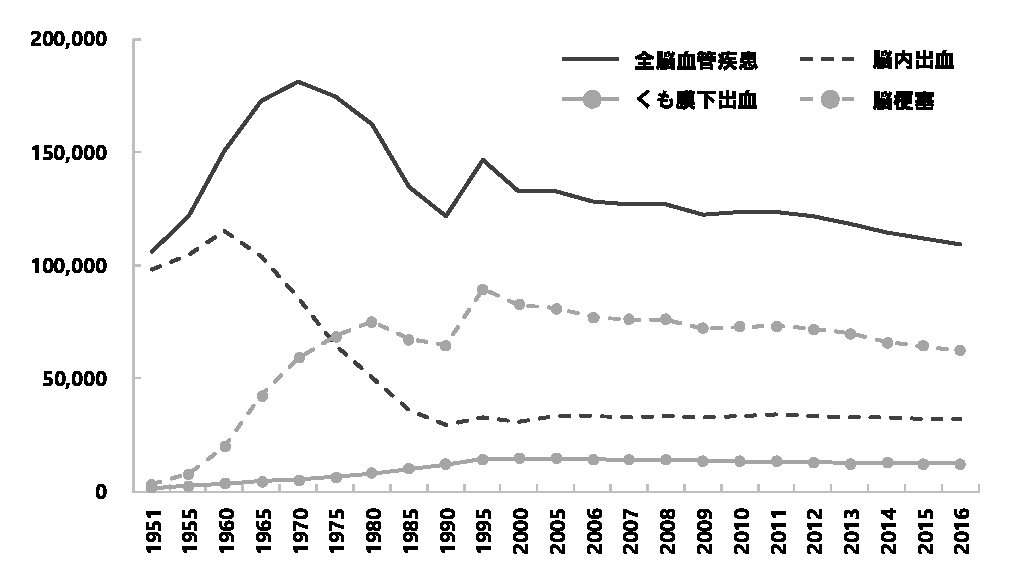
\includegraphics[width=0.95\linewidth]{./Chap1/fig/number_death.eps}
\caption{日本における脳卒中分類別死亡率の推移}
\label{fig:number_death}
\end{center}
\end{figure}

脳卒中のリハビリテーション(以下リハビリ)は,急性期,回復期,維持期の三つの区分に分けられている.
脳卒中発症直後の急性期からリハビリを行うことが勧められている\cite{脳卒中2009}.
脳卒中発症2週間後から5, 6ヶ月までの回復期において,
片側の上下肢が動かない片麻痺の患者は理学療法士から受けるリハビリを行うことで下肢の機能の再建を行う.
下肢機能の再建のための訓練により,Activities of Daily Livingの向上,Quality of Lifeの向上が見込める.
さらには維持期に長期的に運動機能を維持することで,社会復帰を図る.

%%%%%%%%%%%%%%%%%%%%%%%%%%%%%%%%%%%%%%%%%%%%%%%%%%%%%%%%%%%%%%%%%%%%%%%%%%%%%%%%%%%%%%%%%%%%%%%%%%%%%%%%%%%%%%%%%%%%%%%%%%%%%%%%%%%
\section{リハビリテーションへのロボットの介入}
\label{sec:robotics_chap1}
近年のロボット技術の向上により,リハビリの領域にロボットを介入することが期待されている.
ロボット介入の意義は
\begin{itemize}
	\item 多関節の同時コントロールが可能
	\item 正常軌道の運動が可能
	\item 負荷量の調節と負荷量の維持が可能
	\item 結果の提示,つまりフィードバックが可能
\end{itemize}
という4点である\cite{道免2015}.\\

すでに歩行運動については,歩行をアシストするロボットを用いることで歩行能力が改善された報告がある\cite{Fisher2011}\cite{Srivastava2016}\cite{有末2015}.

Fisherらは回復期の片麻痺患者に対し,理学療法士による従来のリハビリとアシストロボットを利用したトレッドミルでの歩行によるリハビリ(Robot Assisted Gait Trainig,以下RAGT)を比較した.
アシストロボット(Autoambulator)は患者を吊り下げるハーネスと,股関節・膝関節を補助する外骨格の駆動装置から成る.外観を図\ref{fig:autoambulator}に示す.
どちらの患者群でもリハビリの前後で,8 m歩行,3分歩行,Tinettiバランステストの全てにおいて優位にスコアが上昇した.
なお,理学療法士による従来のリハビリとRAGTによるリハビリとの間ではリハビリ後のスコアに差は無かった.

\begin{figure}[b]
	\begin{center}
		\includegraphics[width=4.5cm]{./Chap1/fig/Autoambulator.PNG}
		\caption{Autoambulatorによるリハビリの様子\cite{Fisher2011}}
		\label{fig:autoambulator}
	\end{center}
\end{figure}

Srivastavaらも理学療法士のリハビリとRAGTのリハビリを比較している.
麻痺側の足に外骨格(ALEX)を装着し,健常者の軌道から外れた時だけ支援する.
外観を図\ref{fig:ALEX}に示す.
Fisherらの結果と同様,どちらのリハビリでも患者の運動機能は改善したがスコアの上昇に差はなかった.
RAGTのリハビリの方が理学療法士の負担が減ると結論づけている.

\begin{figure}[b]
	\begin{center}
		\includegraphics[width=8cm]{./Chap1/fig/ALEX.PNG}
		\caption{RAGTのリハビリの様子\cite{Srivastava2016}}
		\label{fig:ALEX}
	\end{center}
\end{figure}

有末らは回復期の片麻痺患者に対し,Honda歩行アシストを用いた歩行練習を検討した.
Honda歩行アシストは股関節の屈曲・伸展運動を大腿部のフラームを通じて補助する.
装着者の歩行周期に合わせて,股関節の屈曲・伸展のタイミングを補正する\cite{渡邊2016}.
訓練前の歩行速度が60 m/min未満の患者において,歩行速度や歩行の幅が増加した.\\

本研究では回復期のリハビリにおける片麻痺患者の起立動作に着目する.
運動機能が低下すると生活範囲が狭まる\cite{Guralnik1994}ため,日常生活の中で活動の起点となる起立動作の訓練が必要である.
入院中や退院後について理学療法士がいない中でも,廃用性症候群を防ぐために起立動作を行わなければならない.
よって,自立を促すための起立動作の支援への要求があり,片麻痺患者の起立動作を支援する機器の開発が重要である.
%次項にて起立動作の支援機器に関する従来研究について述べる.

\clearpage

%%%%%%%%%%%%%%%%%%%%%%%%%%%%%%%%%%%%%%%%%%%%%%%%%%%%%%%%%%%%%%%%%%%%%%%%%%%%%%%%%%%%%%%%%%%%%%%%%%%%%%%%%%%%%%%%%%%%%%%%%%%%%%%%%%%

\section{起立動作の支援機器に関する従来研究}
\label{sec:related_research_chap1}

起立動作の支援機器に関する従来研究について述べる.
%支援機器は大きく分けて2つに分類することができる.
多くの片麻痺患者は非麻痺側の足からの感覚入力が受け取れないため,姿勢制御が不安定になる\cite{Chou2003}.
そのため,健側の足に体重を乗せて立ち上がるので動作は左右で非対称なものとなり,健側の足に大きな負担がかかってしまう.
リハビリテーションにおいては麻痺側の足をいかに活用し,左右対称な動きにするかが重要である.

起立動作の支援機器の従来研究として,起立動作を外骨格などにより支援するもの\cite{Tsukahara2010}と座面が上昇することで支援するもの\cite{Shiraishi2016}がある.

TsukaharaらはロボットスーツHALを用いて完全片麻痺患者の起立動作を支援するシステムを開発した.
腰・膝・足関節の運動を支援するHALと,前方に倒れないようにするために腰をサポートするハーネスでシステムは構成されている.外観を図\ref{fig:HAL}に示す.
システムは脛が前傾し,足部の圧力中心がある閾値を超えるかどうか判断することで使用者の動作意図を読み取り,起立動作を支援する.
完全片麻痺患者1名に対して実験を行い,安定して立ち上がることができたと報告している.

\begin{figure}[b]
	\begin{center}
		\includegraphics[width=10cm]{./Chap1/fig/HAL.PNG}
		\caption{HALを用いた支援の様子\cite{Tsukahara2010}}
		\label{fig:HAL}
	\end{center}
\end{figure}

Shiraishiらは座面が直線的に移動することで片麻痺患者の起立動作を支援するシステムを開発した.
床反力から使用者の動作意図を読み取り,座面が臀部を直線的に押し上げることで起立動作を支援する.外観を図\ref{fig:Handrail}に示す.
2名の片麻痺患者と1名の四肢麻痺患者に対して実験を行い,麻痺側と非麻痺側の足の使用率の差が減少したと報告している.

\begin{figure}[b]
	\begin{center}
		\includegraphics[width=10cm]{./Chap1/fig/Handrail.PNG}
		\caption{支援の様子\cite{Shiraishi2016}}
		\label{fig:Handrail}
	\end{center}
\end{figure}


これらの従来研究は関節に力を補助するような筋力増強が主である.
運動を最初から最後まで支援することなり,支援のしすぎとなる可能性がある.
しかし,運動を支援する際には,運動のメカニズムを理解したうえで支援することが重要である.



\clearpage
%%%%%%%%%%%%%%%%%%%%%%%%%%%%%%%%%%%%%%%%%%%%%%%%%%%%%%%%%%%%%%%%%%%%%%%%%%%%%%%%%%%%%%%%%%%%%%%%%%%%%%%%%%%%%%%%%%%%%%%%%%%%%%%%%%%
\section{研究の目的}
\label{sec:objective_chap1}

\ref{sec:background_chap1}節で,脳卒中により片麻痺となった患者のリハビリの重要性について述べた.
\ref{sec:robotics_chap1}節で,歩行動作のリハビリに投入されるロボットについて,\ref{sec:related_research_chap1}節で起立動作の支援機器について述べた.
しかし,従来の支援機器ではヒトの運動のメカニズムを理解した上で動作を支援していないことが明らかになった.\\

本研究ではヒトの運動のメカニズムを理解し,片麻痺患者のリハビリを日常的に支援する機器を開発する.
本研究の対象者は回復期の片麻痺患者であり,入院中に日常的に使用することでリハビリを行うことを目指す.
まず,片麻痺患者が理学療法士によるリハビリを受けてどのように起立動作が変化するかを調査する.
起立動作の変化をヒトの運動のメカニズムに沿って捉えることで,リハビリの効果を検証する.
次に,片麻痺患者の起立動作のリハビリにおける理学療法士の技能を解析する.
理学療法士は片麻痺患者の起立動作の最初から最後まで力を入れているわけではなく,特定のタイミングで起立動作を支援している.
特定のタイミングで支援する技能を解析することで,起立動作の支援機器に応用する.
そして,起立動作の支援機器を開発し,機器の有効性を検証する.

以上より,本研究の目的を以下のように3つ設定する.
%\begin{center}
%\doublebox{
%	\begin{tabular}{c}
		\begin{enumerate}
			\item 理学療法士の介入による片麻痺患者への影響を調査
			\item 理学療法士の技能を解析
			\item 理学療法士の技能を活用した,起立動作の支援機器の開発
		\end{enumerate}
%	\end{tabular}
%}
%\end{center}





\clearpage


%%%%%%%%%%%%%%%%%%%%%%%%%%%%%%%%%%%%%%%%%%%%%%%%%%%%%%%%%%%%%%%%%%%%%%%%%%%%%%%%%%%%%%%%%%%%%%%%%%%%%%%%%%%%%%%%%%%%%%%%%%%%%%%%%%%
\section{本論文の構成}

本論文は全6章から構成されている.本論文の構成を図\ref{fig:thesis_flow}に示す.

第1章では,本研究の背景と従来研究,目的について述べた.

第2章では,問題設定を明らかにし,本研究におけるアプローチについて述べる.

第3章では,理学療法士のリハビリテーションによる片麻痺患者への影響について述べる.

第4章では,理学療法士のリハビリテーションの技能について述べる.

第5章では,起立動作の支援機器への応用と有効性を検証するために行った実験について述べる.

第6章では,本研究の結論と今後の展望について述べる.

%\clearpage


\begin{figure}[b]
\begin{center}
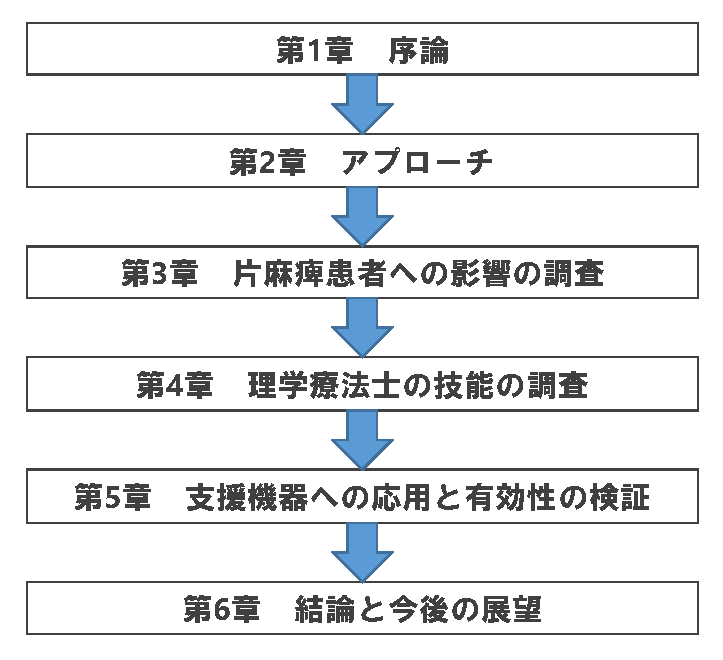
\includegraphics[width=8cm]{./Chap1/fig/thesis_flow.eps}
\caption{本論文の構成}
\label{fig:thesis_flow}
\end{center}
\end{figure}

\clearpage



%%%%%%%%%%%%%%%%%%%%%%%%%%%%%%%%%%%%%%%%%%%%%%%%%%%%%%%%%%%%%%%%%%%%%%%%%%%%%%%%%%%%%%%%%%%%%%%%%%%%%%%%%%%%%%%%%%%%%%%%%%%%%%%%%%%
%%% Local Variables:
%%% mode: katex
%%% TeX-master: "../thesis"
%%% End:

\chapter{本研究のアプローチ}
\label{chap:approach}
\minitoc

\thispagestyle{empty}

\newpage
%%%%%%%%%%%%%%%%%%%%%%%%%%%%%%%%%%%%%%%%%%%%%%%%%%%%%%%%%%%%%%%%%%%%%%%%%%%%%%%%%%%%%%%%%%%%%%%%%%%%%%%%%%%%%%%%%%%%%%%%%%%%%%%%%%%
\section{はじめに}
\label{sec:intro_chap2}

本章では,ヒトの運動のメカニズムを理解し,片麻痺患者の回復期のリハビリテーション(以下リハビリ)を日常的に支援する機器を開発するアプローチについて述べる.

%\ref{sec:problem_setteing_chap2}節にて,本研究における問題設定について述べる.

\ref{sec:approach_chap2}節にて,本手法のアプローチと解決すべき課題について述べる.
\ref{subsec:investigate_chap2}項にて,理学療法士のリハビリテーションにおける片麻痺患者への影響の調査について述べる.
\ref{subsec:analysys_chap2}項にて,理学療法士の技能を解析するアプローチについて述べる.
\ref{subsec:development_chap2}項にて,理学療法士の技能を応用する支援機器の開発のアプローチについて述べる.

\ref{sec:outro_chap2}節にて,本章のまとめを述べる.

\clearpage

%%%%%%%%%%%%%%%%%%%%%%%%%%%%%%%%%%%%%%%%%%%%%%%%%%%%%%%%%%%%%%%%%%%%%%%%%%%%%%%%%%%%%%%%%%%%%%%%%%%%%%%%%%%%%%%%%%%%%%%%%%%%%%%%%%%

%\section{問題設定}
%\label{sec:problem_setteing_chap2}
%第1章にて,が重要であることを述べた.\\
%
%また,\ref{sec:related_research_chap1}節にて,を述べた.などが例として挙げられる.\\
%
%また,同様に\ref{sec:related_research_chap1}節にて,であることを述べた.従って,本研究では利用する.\\
%
%上記を踏まえて,以下に本研究の問題設定をまとめる.
%\begin{itemize}
%\item 患者への影響を調査
%\item 技能を調査
%\item 支援機器を開発
%\end{itemize}
%
%このような問題設定の下,手法を提案する.
%
%
%\clearpage


%%%%%%%%%%%%%%%%%%%%%%%%%%%%%%%%%%%%%%%%%%%%%%%%%%%%%%%%%%%%%%%%%%%%%%%%%%%%%%%%%%%%%%%%%%%%%%%%%%%%%%%%%%%%%%%%%%%%%%%%%%%%%%%%%%%
\section{アプローチ}
\label{sec:approach_chap2}
\ref{sec:objective_chap1}節にて述べた通り,本研究の目的は理学療法士の介入による片麻痺患者への影響を調査,理学療法士の技能を解析,理学療法士の技能を活用した,起立動作の支援機器の開発の三つである.
それぞれの目的を達成するためのアプローチを次節で述べていく.\\

%\clearpage
%%%%%%%%%%%%%%%%%%%%%%%%%%%%%%%%%%%%%%%%%%%%%%%%%%%%%%%%%%%%%%%%%%%%%%%%%%%%%%%%%%%%%%%%%%%%%%%%%%%%%%%%%%%%%%%%%%%%%%%%%%%%%%%%%%%
\subsection{片麻痺患者への影響の調査}
\label{subsec:investigate_chap2}

理学療法士のリハビリテーションにより片麻痺患者にどのような影響があるのかを調査することを前述した.本項では,片麻痺患者への影響の調査方法について説明する.\\

起立動作は,年齢,関節角度,床反力,関節トルク,重心軌道,表面筋電図など多くの指標により調べられてきた.しかし,片麻痺患者に対してどの指標がより起立動作の特徴を捉えているか,有用な指標を抽出するような研究は行われていない\cite{長田2012}.

本研究では起立動作を運動学的な観点と表面筋電図から計算される筋シナジー構造から評価する.運動学的な観点の指標として,片麻痺患者の関節角度や重心(Center of Mass,以下CoM)の軌道を用いる.

起立動作のCoMについてはいくつかの報告がなされている.
\textcolor{red}{\cite{Mourey2000}と\cite{Yang2017}を引いて,高齢者や片麻痺患者は上体を深く曲げて起立することを記述}
%高齢者は筋肉量が低下しているため,起立の際には転倒の危険性が発生する.より安定した起立のために,若年者よりも上体を深く曲げることでCoMを足に近づけてから立ち上がる\cite{Mourey2000}.
%さらに,片麻痺患者になると健常な高齢者よりもCoMが足に近づいてから立ち上がることが分かっている\cite{Yang2017}.
\\

起立動作中の筋電図(Electromyogram,以下EMG)については以下のような報告がある.
\textcolor{red}{\cite{Silva2013}と\cite{Gross1998}を引いて,前脛骨筋の活動タイミングなどについて記述.}\\
%Silvaらは健常者と片麻痺患者を対象とし,ヒラメ筋と前脛骨筋のEMGを計測した\cite{Silva2013}.片麻痺患者において健常者よりも,麻痺と非麻痺の両側のヒラメ筋の活動タイミングが早く,麻痺側の前脛骨筋の活動タイミングが遅かったと報告している.
%また,Grossらは若年者と片麻痺患者を対象として前脛骨筋と大腿四頭筋のEMGを計測した\cite{Gross1998}.片麻痺患者において,健側の足の位置を変えることで前脛骨筋の大腿四頭筋の活動が増加することを報告した.

本研究ではヒトの運動のメカニズムを理解するべく,筋シナジー仮説を用いる.


\textcolor{red}{筋シナジー仮説とは何かを説明.}
\\

運動学的な指標や筋シナジー構造の詳細な算出方法や計測実験については第\ref{chap:investigation}章にて述べる.

%\clearpage
%%%%%%%%%%%%%%%%%%%%%%%%%%%%%%%%%%%%%%%%%%%%%%%%%%%%%%%%%%%%%%%%%%%%%%%%%%%%%%%%%%%%%%%%%%%%%%%%%%%%%%%%%%%%%%%%%%%%%%%%%%%%%%%%%%%
\subsection{理学療法士の技能解析}
\label{subsec:analysys_chap2}

片麻痺患者のリハビリテーション中において,理学療法士はどのような介入を行っているのかを調査することを前述した.本項では,理学療法士の技能の解析方法について説明する.\\

理学療法士の技能について,Tsusakaらは起立動作における理学療法士のスキル分析をしている\cite{Tsusaka2015}.
\textcolor{red}{スキル分析について記述.}\\

本研究では理学療法士の技能の調査方法として片麻痺患者に介入する腕の筋肉の表面筋電図を計測する.
理学療法士は図\ref{fig:view}に示すように,片麻痺患者の麻痺側の膝と骨盤後面に介入する.上肢の曲げ伸ばしをどのタイミングで行っているかを調査するため,理学療法士の腕の筋肉の表面筋電図を計測する.
\\

\begin{figure}[b]
	\begin{center}
		\includegraphics[width=8cm]{./Chap2/fig/view.eps}
		\caption{理学療法士による介入の様子}
		\label{fig:view}
	\end{center}
\end{figure}

理学療法士の技能の詳細な調査方法は第\ref{chap:analysys}章にて述べる.

%\clearpage

%%%%%%%%%%%%%%%%%%%%%%%%%%%%%%%%%%%%%%%%%%%%%%%%%%%%%%%%%%%%%%%%%%%%%%%%%%%%%%%%%%%%%%%%%%%%%%%%%%%%%%%%%%%%%%%%%%%%%%%%%%%%%%%%%%%
\subsection{起立動作の支援機器の開発}
\label{subsec:development_chap2}

本研究では理学療法士の技能を活用した,起立動作の支援機器の開発について前述した.
本項では,技能を活用した支援機器の従来研究について説明する.\\

\textcolor{red}{看護師の技能を活かした起立動作の支援システムを引く\cite{Chugo2007}.
	理学療法士のスキル活かした起立アシストロボットの開発を引く\cite{津坂2017}.
}\\



起立動作の支援機器の開発についての詳細な方法は第\ref{chap:development}章にて述べる.

\clearpage

%%%%%%%%%%%%%%%%%%%%%%%%%%%%%%%%%%%%%%%%%%%%%%%%%%%%%%%%%%%%%%%%%%%%%%%%%%%%%%%%%%%%%%%%%%%%%%%%%%%%%%%%%%%%%%%%%%%%%%%%%%%%%%%%%%%
\section{おわりに}
\label{sec:outro_chap2}

本章では,本研究のアプローチについて述べた.

%まず\ref{sec:problem_setteing_chap2}節にて,本研究において解決するべき課題について述べた.

\ref{sec:approach_chap2}節にて,本手法のアプローチと解決すべき課題について述べた.
\ref{subsec:investigate_chap2}節にて,理学療法士によるリハビリ中の片麻痺患者の起立動作の変化を調査するアプローチについて述べた.
\ref{subsec:analysys_chap2}項にて,理学療法士の技能を解析するためのアプローチについて述べた.
\ref{subsec:development_chap2}項にて,支援機器を開発するアプローチについて述べた.\\

次章では,技能解析について詳しく説明する.

\clearpage

%%%%%%%%%%%%%%%%%%%%%%%%%%%%%%%%%%%%%%%%%%%%%%%%%%%%%%%%%%%%%%%%%%%%%%%%%%%%%%%%%%%%%%%%%%%%%%%%%%%%%%%%%%%%%%%%%%%%%%%%%%%%%%%%%%%
%%% Local Variables:
%%% mode: katex
%%% TeX-master: "../thesis"
%%% End:

\chapter{����J�����ɂ��v���̂��߂̉摜����}
\label{chap:ImageProcessing}
\minitoc

\thispagestyle{empty}

\newpage
%%%%%%%%%%%%%%%%%%%%%%%%%%%%%%%%%%%%%%%%%%%%%%%%%%%%%%%%%%%%%%%%%%%%%%%%%%%%%%%%%%%%%%%%%%%%%%%%%%%%%%%%%%%%%%%%%%%%%%%%%%%%%%%%%%%
\section{�͂��߂�}
\label{sec:}

%\textcolor{red}{�{�͉͂��M�C������\��ł��D�}���ς��DOCamCalib�̎��ƃ��f���m�F}

�{�͂ł́C����J�����Ŏ擾�����摜�ɂ���ăI�[������3�����v�����s�����߂ɗp������W�n��K�v�ȃp�����[�^�C�摜�����ɂ‚��ďq�ׂ�D
%�{�����ł́C�n��̈قȂ镡���n�_�ɋ���J������ݒu���C�����������Ƃ��ăI�[�������B�e�����摜����͉摜�Ƃ���D
%���͉摜�̂���1�΂̓��͉摜��p���ăI�[�����̃X�e���I�v�����s�����C�J�����̈ʒu��p�����قȂ邽��2��̃J�����ɋ��ʂȍ��W�n��݂���D��������N�e�B�t�@�C�h���W�n�ƌĂԁD
%�ݒu���ꂽ�ʒu��p���̈قȂ�2��̃J�����摜��p���ăX�e���I�v�����s�����߁C2��̃J�����ɋ��ʂȍ��W�n��݂��C��������N�e�B�t�@�C�h���W�n�ƌĂԁD
%�{�����ł͋���摜��p�����v�����ȒP�ɂ��邽�߂ɁC�摜�����ɂ���ē��͉摜�����N�e�B�t�@�C�h���W�n�摜�֕ϊ����C����ɋ��჌���Y�ɋN������c�݂��������������e�摜�ւƕϊ�����D
%����摜�͋��჌���Y�̌��w���f���ɂ���ĕω����邽�߁C�g�p���鋛�჌���Y�̃��f���Ɋ�Â��ĉ摜�̍��W�ϊ���c�݂̏������s���D
%�܂��C�摜��ϊ�����ۂɕK�v�ȃJ�����̓����p�����[�^��O���p�����[�^�𐄒肷��D\\

�܂�\ref{sec:gaiyou2}�߂ł͖{�͂ōs���摜�����̊T�v�ɂ‚��ďq�ׂ�D

����\ref{sec:rectified}�߂Ŗ{�����ŋ���摜�΂𕽍s�X�e���I�y�A�Ƃ��Ĉ������߂ɒ�`������W�n�ɂ‚��ďq�ׂ�D

\ref{sec:fisheye_model}�߂ł́C��ʓI�ȃJ�����Ƌ���J�����̈Ⴂ�ɂ‚��ďq�ׂ���C���჌���Y�ɂ��c�݂̃��f���ɂ‚��Đ�������D�����Ė{�����ŗp���鋛��J�����̃��f���ɂ‚��ďq�ׂ�D

\ref{sec:calibration}�߂Ŗ{�����ɂ�����摜�����ɕK�v�ȃp�����[�^�ƁC�����̐�����@�ɂ‚��ďq�ׂ�D

\ref{sec:translation}�߂ł́C���͉摜�΂𕽍s�X�e���I�摜�΂ւƕϊ�����摜������@�ɂ‚��ďq�ׂ�D�摜�̕ϊ��ɂ�\ref{sec:rectified}�߂Œ�`�������W�n��\ref{sec:calibration}�߂Ő��肵���p�����[�^��p����D

%���̍��W�n�ւ̉摜�̕ϊ����@�ɂ‚��ďq�ׂ�D�ϊ��ɂ�\ref{sec:calibration}�߂Ő��肵���p�����[�^��p����D

�Ō��\ref{sec:undistortion}�߂ł́C���͉摜���狛�჌���Y�ɂ��c�݂���菜���������e�摜�ւƕϊ������@�ɂ‚��ďq�ׂ�D
%�Ō��\ref{sec:backsubtraction}�߂ł́C�����_���o�̂��߂ɉ摜������I�[�����̈�𒊏o����w�i�����ɂ‚��ďq�ׂ�D
\clearpage
%%%%%%%%%%%%%%%%%%%%%%%%%%%%%%%%%%%%%%%%%%%%%%%%%%%%%%%%%%%%%%%%%%%%%%%%%%%%%%%%%%%%%%%%%%%%%%%%%%%%%%%%%%%%%%%%%%%%%%%%%%%%%%%%%%%
\section{����J�����ɂ��v���̂��߂̉摜�����̊T�v}
\label{sec:gaiyou2}

��Ď�@�ł�2��̃J�����ŎB�e����1�΂̃I�[�����摜����Ή��_�����o���C�O�p���ʂ̌�������I�[������3�����`����v������D
���̂悤�ȃX�e���I�v���ɂ����ẮC2��̃J�����̍����𑵂����ꂼ��̌��������s�ɂȂ�悤�ɐݒu�������s�X�e���I�v���������s���Ă���D
�J�����𕽍s�X�e���I�y�A�Ƃ��邱�ƂŃG�s�|�[���􉽂ƌĂ΂��􉽏��������������m�ɗ��p�”\�ƂȂ�C
�摜�Ԃ���̑Ή��_���o�̑��x�␸�x�̌��オ���҂����D
�����Ŗ{�����ɂ����Ă��C�J�����𕽍s�X�e���I�y�A�Ƃ��v������D\\

������2��̃J�����̐ݒu�ʒu��p�x�𒲐��ł���ꍇ�C�����I�Ɍ����ɕ��s�X�e���I�y�A�ƂȂ�悤�J������ݒu���邱�Ƃ͗L���Ȏ�i�ł���D
�������I�[�����v���ɏ\���Ȏ����𓾂邽�߂ɂ́C�ݒu����J�����Ԃ̋�����傫������K�v������C
�����I�Ɍ����ȕ��s�X�e���I�y�A�Ƃ��邱�Ƃ͍���ł���ƍl������D
�����Ŗ{�����ł͉摜�����ɂ���ĉ摜�΂𕽍s�X�e���I�J�����ɂ���Ď擾�����摜�΂ɂȂ�悤�ϊ�����i\ref{sec:translation}�߁j�D
�摜�����ɂ���ĉ摜�΂𕽍s�����邽�߂ɂ́C�L�����u���[�V�����ɂ���ăJ�������L�̘c�݂�C�J�����̐ݒu�ʒu���]�Ƃ������p�����[�^�𐄒肷��K�v������i\ref{sec:calibration}�߁j�D
���̂悤�ȃp�����[�^���擾���邽�߂ɁC�܂��J���������s�ƂȂ���W�n��{�����Ŏg�p���鋛�჌���Y�ɂ��c�݂̃��f�����`����i\ref{sec:rectified}�߁C\ref{sec:fisheye_model}�߁j�D\\

�{�����ł͋���J�������g�p���邽�߁C������摜�͑傫�Șc�݂������Ă���D
��ʓI�ɋ���摜����̑Ή��_���o�́C�ʏ�̃����Y�ŎB�e�����摜�΂���̑Ή��_���o�ɔ�ד�Փx�������Ȃ�D
�����Ŗ{�����ł͑Ή��_���o�̑O�ɁC���s�������摜�΂���摜�����ɂ���ċ���摜���狛�჌���Y���L�̘c�݂���������i\ref{sec:undistortion}�߁j�D
�c�݂̏����ɂ́C�L�����u���[�V�����ɂ���Ď擾�����p�����[�^��p����D




\clearpage
%%%%%%%%%%%%%%%%%%%%%%%%%%%%%%%%%%%%%%%%%%%%%%%%%%%%%%%%%%%%%%%%%%%%%%%%%%%%%%%%%%%%%%%%%%%%%%%%%%%%%%%%%%%%%%%%%%%%%%%%%%%%%%%%%%%%
\section{���N�e�B�t�@�C�h���W�n}
\label{sec:rectified}

�{�����ł͒n��̈قȂ镡���n�_�ɋ���J������ݒu���C�S�ẴJ�����Ŏ����������Ƃ��ĎB�e�����I�[�����̉摜����͉摜�Ƃ���D
�����n�_����B�e�������͉摜�̂����C2�n�_����B�e����1�΂̓��͉摜��p���ăX�e���I�v�����s���D
�X�e���I�v���ł͈�ʓI�ɁC�����Ɛ��x�����コ���邽�߂ɃG�s�|�[���􉽂ƌĂ΂��􉽊w�I�ȍS���������p������\cite{cox1996}�D%���̃G�s�|�[���S�����摜��ŊȒP�Ɉ�����Ƃ������R����C�J�����𕽍s�ɐݒu�������s�X�e���I�v����
�{�����ł́C�G�s�|�[���S���̉摜��ł̈�����e�Ղɂ��邽�߂ɁC�J�����𕽍s�ɐݒu�������s�X�e���I�v�����s���D
�������}\ref{fig:camera_install}�̂悤�ɃI�[�����͍��x100 km�ȏ�̏��Ŕ������邽��\cite{jones1971}�C�O�p���ʂɂ��v���ɏ\���Ȏ����𓾂邽�߂�2��̃J�����͑傫�������������Đݒu����K�v������D
���̂���2��̃J�����̎p����ݒu���ɒ��߂��邱�Ƃɂ���Đ��m�ȕ��s�X�e���I�y�A�ɂ��邱�Ƃ͍���ł���D
�����ʼn摜�����ɂ����͉摜�΂𕽍s�X�e���I�摜�΂ւƕϊ�����K�v������D\\
%�������I�[�����͍��x100 km�ȏ�̏��ɔ������錻�ۂł��邽��[���p�\��]�C�X�e���I�v�����邽�߂ɂ̓J�����Ԃ̋�������ɑ傫������K�v������C�J�����𕽍s�X�e���I�y�A�ɂ��邱�Ƃ͍���ł���D�����ʼn摜�����ɂ���ē��͉摜�΂𕽍s�X�e���I�摜�΂ւƕϊ�����K�v������D\\

\begin{figure}[b]
\begin{center}
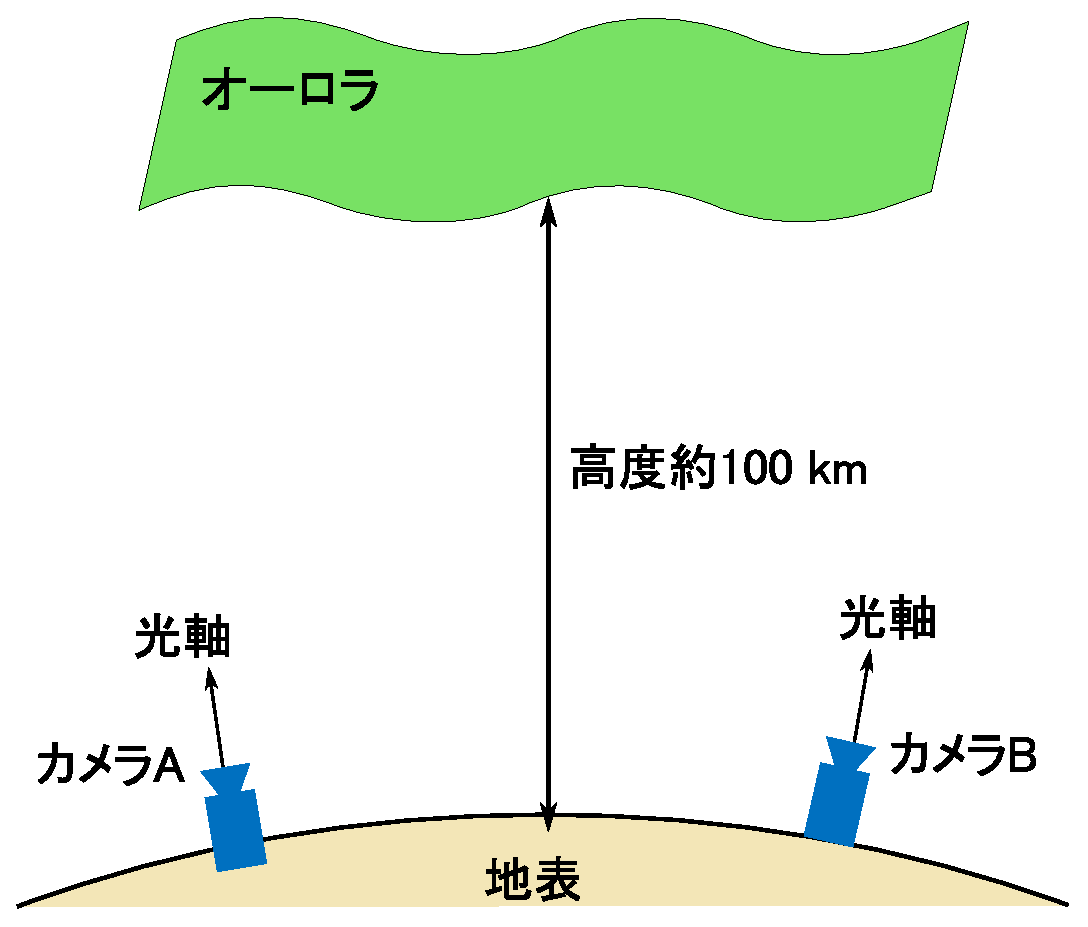
\includegraphics[width=7cm]{./chap3/eps/CameraInstall.eps}
\vspace{5mm}
\caption{�I�[�����̍��x�ƃJ�����ݒu�ʒu�̊֌W}
\label{fig:camera_install}
\end{center}
\end{figure}

���͉摜�΂𕽍s�X�e���I�摜�΂ւƕϊ����邽�߂ɁC2��̃J�����ɋ��ʂȍ��W�n��݂���D
���̍��W�n�����N�e�B�t�@�C�h���W�n�ƌĂԁD
2��̃J���������ꂼ��J����A�C�J����B�ƌĂԂ��ƂƂ���D�J����A�C�J����B�ƃ��N�e�B�t�@�C�h���W�n�Ƃ̊֌W��}\ref{fig:RicthifiedCoordinate}�Ɏ����D
���N�e�B�t�@�C�h���W�n�̌��_���J����A�̌��w���S�Ƃ��CX�����J����A�̌��w���S����J����B�̌��w���S�֌����������ƒ�`����D
X����Y���ɐ����ŁC�n�\����V�������Ɍ�����������Z�����Ƃ�D
�܂��CY���͉E��n�ɏ]���C���_�ɂ�����n�\�ʂ̐ݒu���ʂ�X���ɐ����ȕ����ƒ�`����D\\

�e�J�����̎p���ƃ��N�e�B�t�@�C�h���W�n�̊֌W��}\ref{fig:rictify_rotate}�Ɏ����D
�ݒu���ꂽ�J����A�̌�����$Z_A$�ŕ\���C$X_A$���C$Y_A$���͓�����摜�̍��W���ɕ��s�Ȏ���\���Ă���D�J����B�Ɋւ��Ă����l�ɕ\���Ă���D
�Ԃ����ŕ\�����������N�e�B�t�@�C�h���W�n�̊e����\���Ă���D
�J����A�̊e�������N�e�B�t�@�C�h���W�n�̊e���ƈ�v����悤�ȉ�]�s���$R_A$�Ƃ���D
�J����B��$X_B$�������N�e�B�t�@�C�h���W�n��$X$���ƈ�v�����C$Y_B$����$Z_B$�������N�e�B�t�@�C�h���W�n��$Y$����$Z$���ɕ��s�ƂȂ�悤�ɂ����]�s���$R_B$�Ƃ���D
�J����A�C�J����B�����ꂼ��$R_A$�C$R_B$��]������Ƃ��C2��̃J�����͕��s�X�e���I�y�A�ƂȂ�D
�܂��C�J�����ԋ�����$d$�Ƃ���ƁC���N�e�B�t�@�C�h���W�n�ɂ����ăJ����A�̍��W��$(0, 0, 0)$�C�J����B�̍��W��$(d, 0, 0)$�ƕ\�����D

%\clearpage

%\textcolor{red}{�i�}�C���\��j}



\begin{figure}[hbp]
\begin{center}
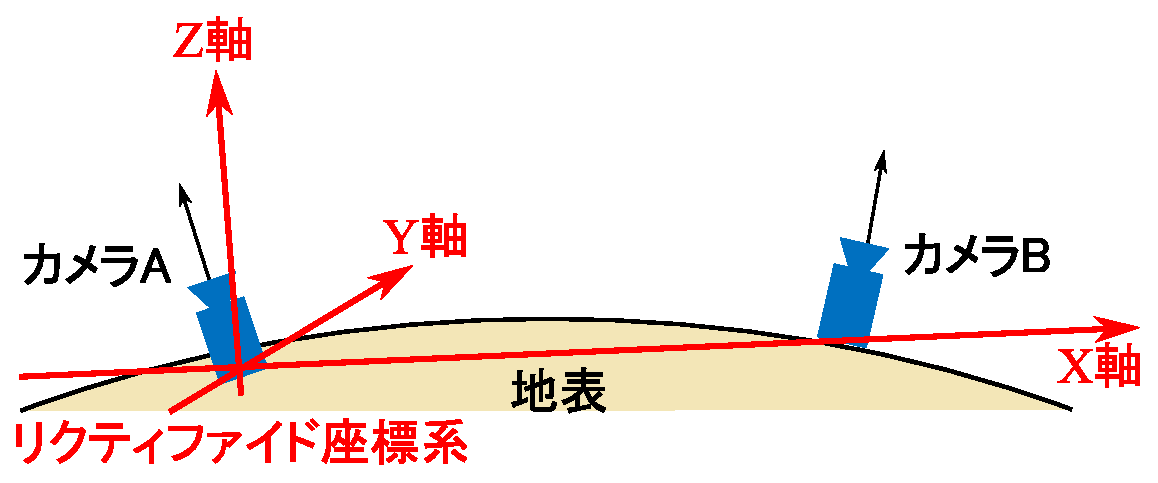
\includegraphics[width=8cm]{./chap3/eps/RicthifiedCoordinate.eps}
\vspace{5mm}
\caption{�J�����̍��W�n�ƃ��N�e�B�t�@�C�h���W�n�̊֌W}
\label{fig:RicthifiedCoordinate}
\end{center}
\end{figure}

%\subsection{���N�e�B�t�@�C�h���W�n�ւ̓��͉摜�ϊ�}
%\label{ssec:rectification}
\begin{figure}[hbp]
\begin{center}
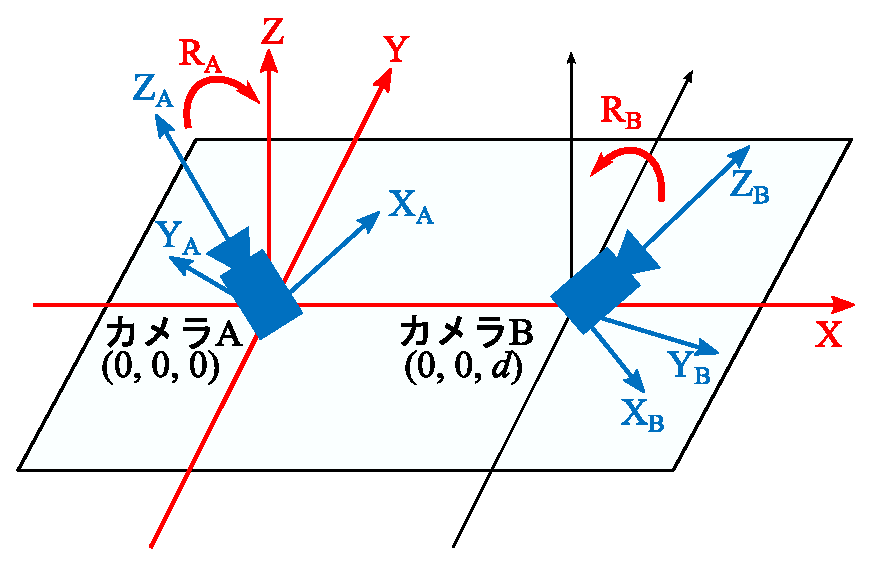
\includegraphics[width=8cm]{./chap3/eps/RecthifyRotate.eps}
\caption{���N�e�B�t�@�C�h���W�n�ւ̃J�����p���̕ϊ�}
\label{fig:rictify_rotate}
\end{center}
\end{figure}

\clearpage

%%%%%%%%%%%%%%%%%%%%%%%%%%%%%%%%%%%%%%%%%%%%%%%%%%%%%%%%%%%%%%%%%%%%%%%%%%%%%%%%%%%%%%%%%%%%%%%%%%%%%%%%%%%%%%%%%%%%%%%%%%%%%%%%%%%
\section{���჌���Y�̃��f��}
\label{sec:fisheye_model}

�摜�����ɂ���ēK�؂ɉ摜��ϊ������m�Ɍv�����s�����߂ɁC�J�����ɓ��˂�������Ƃ��ꂪ���e�����摜���W�Ƃ̊֌W�𐳂����m�邱�Ƃ͕s�Œ��ł���D
�ʏ�̃J�����̃����Y�͈�ʓI�ɓ������e�ˉe�������p�����C�J�����ւ̓��ˌ��̒P�ʃx�N�g�����i$x$, $y$, $z$�j�C�摜���S��($C_u$, $C_v$)�C�œ_������$f$�Ƃ���Ɠ��e�_�̉摜���W�i$u$, $v$�j�͈ȉ��̎�(\ref{eq:NormalCamera})�ɂĕ\�����D

\begin{equation}
\begin{bmatrix}
u\\
v
\end{bmatrix}
=
\begin{bmatrix}
f{x}/{z}\\
f{y}/{z}
\end{bmatrix}
\label{eq:NormalCamera}
\end{equation}

����C��Ď�@�ł͋��჌���Y��p����D���჌���Y�͓��ˌ��������Y�ő傫�����܂��邽�߁C���ˌ��Ɠ��e�_�Ƃ̊֌W����ʓI�ȃJ�����̎�(\ref{eq:NormalCamera})�Ƃ͈قȂ�D
�ʏ�̃����Y�Ƌ��჌���Y�ɂ����ˌ��Ɠ��e�_�Ƃ̊֌W�̈Ⴂ��}\ref{fig:lensmodel}�Ɏ����D\\

\begin{figure}[b]
  \centering
  \subfigure[�ʏ�̃����Y�̎ˉe���f��]{
    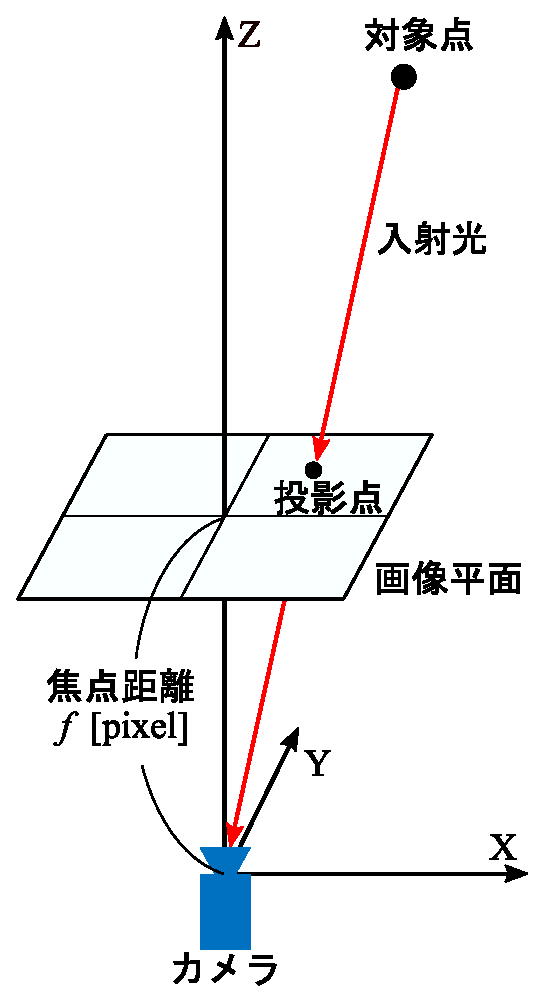
\includegraphics[width=4cm]{./chap3/eps/PerspectiveModel.eps}
  \label{fig:perspective_model}}
\hspace{2cm}
  \subfigure[���჌���Y�̎ˉe���f��]{
    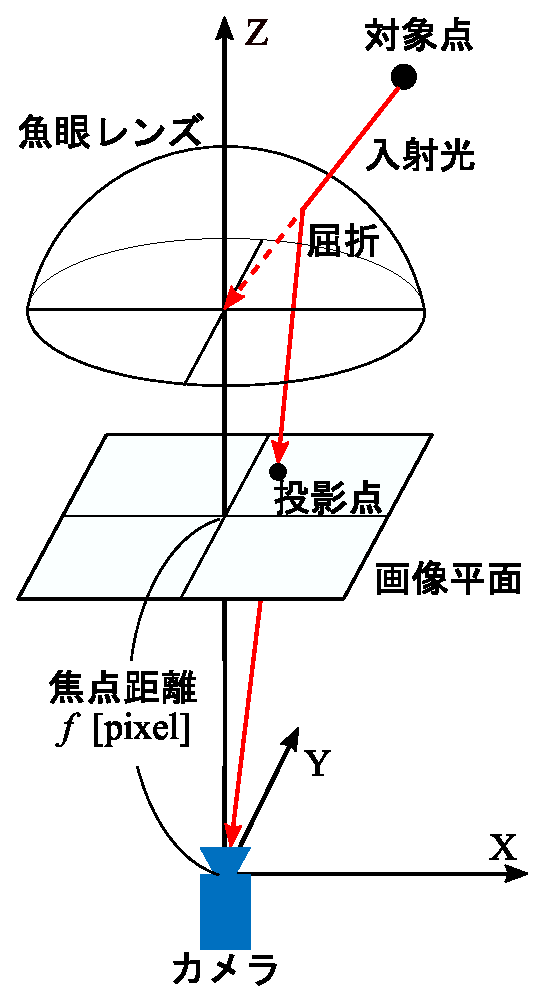
\includegraphics[width=4cm]{./chap3/eps/FisheyeModel.eps}
  \label{fig:fisheye_model}}
%\vspace{10mm}
  \caption{�ʏ�̃����Y�Ƌ��჌���Y�̎ˉe�̈Ⴂ}
  \label{fig:lensmodel}
\end{figure}

���჌���Y�Ƃ́C�L�`�ɖ�$180^{\circ}$���x�̍L����p�������������Y�̂��Ƃ��w�����C�����‚��̎�ނɕ��ނ����D
�C���[�W�T�[�N���a����ʂ̑Ίp�������傫�����჌���Y�͑Ίp���჌���Y�ƌĂ΂�C
��ʓI�ȃJ�������l�ɉ�ʑS�̂ɉf�����f��D
���΂ɃC���[�W�T�[�N������ʂ̍����C���������������჌���Y�͉~�����჌���Y�ƌĂ΂�C��p���̑S�Ẳf�����摜���̉~�`�̗̈�ɉf��D
�Ίp����摜�Ɖ~������摜�̈Ⴂ��}\ref{fig:DiagonalCircle}�Ɏ����D
�B��������p�͈قȂ邪�C�ǂ���̋�������ł����Ă�������摜�͋��჌���Y���L�̘c�݂�L���Ă���C
�c�݂̓����Y�̎ˉe�����Ɉˑ�����D\\



��L�̒ʂ苛�჌���Y�͎ˉe�����ɂ���Ă����ނ����D
�Ⴆ�΃����Y�𔼋��ʂƉ��肵���ꍇ�ɁC������̐}�`�����̂܂ܕ��ʂɎˉe���鐳�ˉe������C���ʏ�̋��������������e�����p�ɂ��𑜓x�̈Ⴂ�̂Ȃ��������ˉe�����C���̖ʐς����̊p�ɔ�Ⴗ�铙���̊p�ˉe�����Ȃǂ̎ˉe���������݂���D
���̎ˉe�����̈Ⴂ������J�����ɂ���ĎB�e���ꂽ�摜�̎��“��L�̘c�݂�ω�������D
���჌���Y�̓��ˌ��Ɠ��e�_�̊֌W��}\ref{fig:tourittai}�Ɏ����D
�摜���S$(C_u, C_v)$����̃s�N�Z��������$r$[pixel]�C�J��������������ˌ��ւ̊p�x��
$\theta$ [$rad$]�C���e�_$�iu, v�j$�Ɖ摜���S�����Ԓ�����$X$���ƂȂ��p��$\phi$ [$rad$]�Ƃ��ĕ\���Ă���D
�}\ref{fig:tourittai}����$\theta$��$r$�̊֌W���ˉe�����ɂ���ĈقȂ�C�����̓����Y�ŗL�̘c�݃p�����[�^$k$ [pixel]�ɂ���Ċ֌W�t������D
�ˉe�������̉摜���S����̃s�N�Z������$r$�ƃJ��������������ˌ��ւ̊p�x$\theta$�C�c�݃p�����[�^$k$�̊֌W��\\ref{table:distortion_parameter}�Ɏ����D\\

\begin{figure}[h]
  \centering
  \subfigure[�Ίp���჌���Y�Ŏ擾�����摜]{
    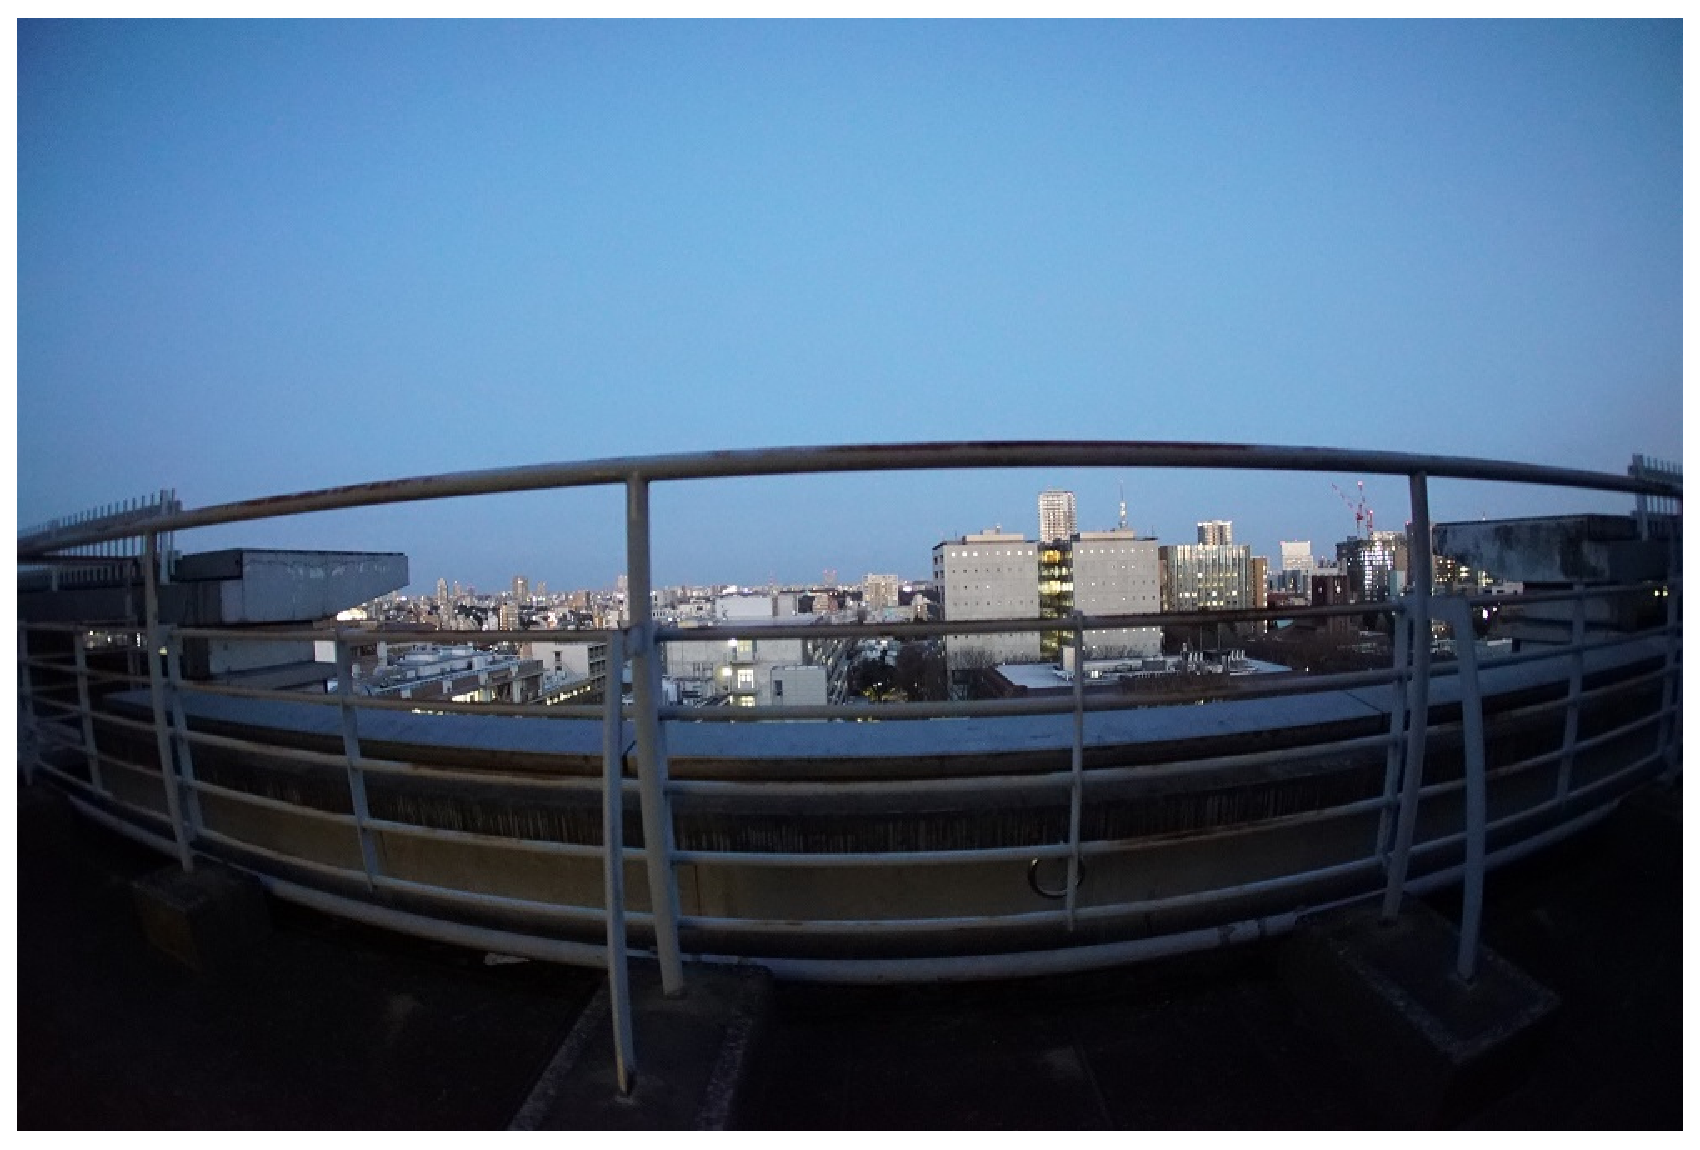
\includegraphics[width=6cm]{./chap3/eps/FisheyeDiagonal.eps}
  \label{fig:Diagonal}}
  \subfigure[�~�����჌���Y�Ŏ擾�����摜]{
    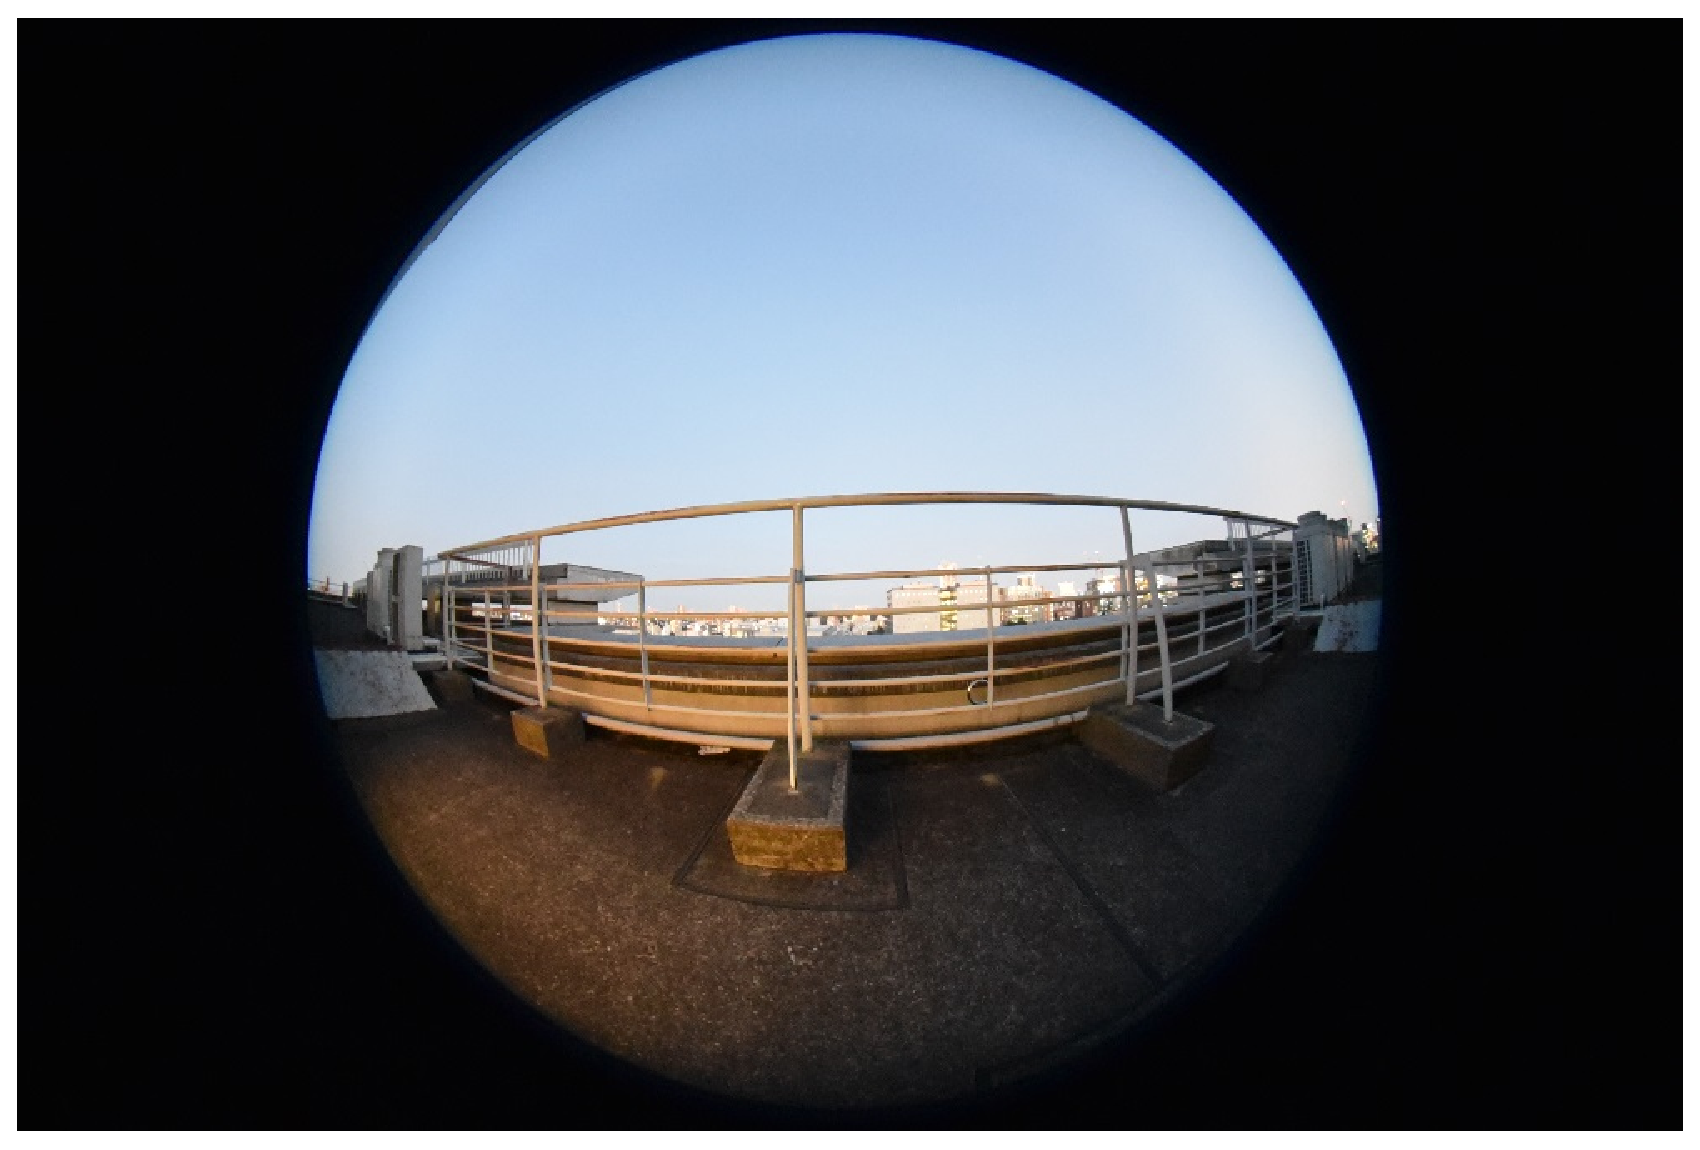
\includegraphics[width=6cm]{./chap3/eps/FisheyeCircle.eps}
  \label{fig:Circle}}
%\vspace{10mm}
  \caption{�Ίp���჌���Y�Ɖ~�����჌���Y�̈Ⴂ}
  \label{fig:DiagonalCircle}
\end{figure}

\clearpage


�}\ref{fig:tourittai}���C���e�_$�iu, v�j$�͓��ˌ��̒P�ʃx�N�g��$�ix, y, z�j$��p���Ĉȉ��̎�(\ref{eq:fisheye_uv})�C��(\ref{eq:fisheye_phi})�ŕ\�����D
�܂��C��(\ref{eq:fisheye_uv})����$r$�͕\\ref{table:distortion_parameter}�����ˌ��ƌ����Ƃ̊p�x$\theta$�Ƙc�݃p�����[�^$k$�ɂ���ĎZ�o�����D
����ăJ�����ŗL�̘c�݃p�����[�^$k$�𐄒肷�邱�Ƃŋ���摜��̃s�N�Z���Ɠ��ˌ��̕����x�N�g������ӂɊ֘A�t���邱�Ƃ��”\�ł���D\\

\begin{figure}[tb]
  \centering
  \subfigure[���ˌ��̓��e�̗l�q]{
    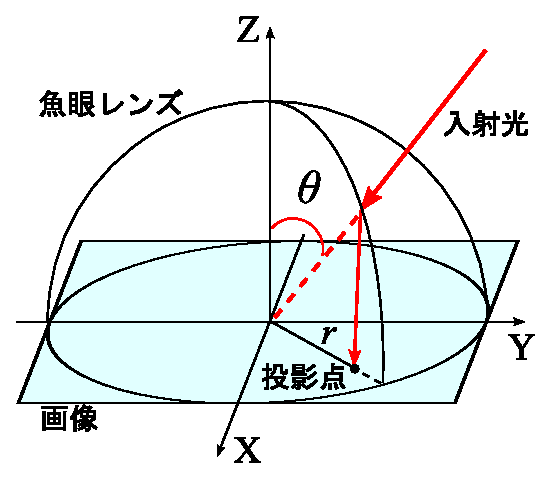
\includegraphics[width=6cm]{./chap3/eps/nyusya.eps}
  \label{fig:nyuusyakou}}
  \subfigure[���e�_$(u, v)$�ƃs�N�Z������$r$�̊֌W]{
    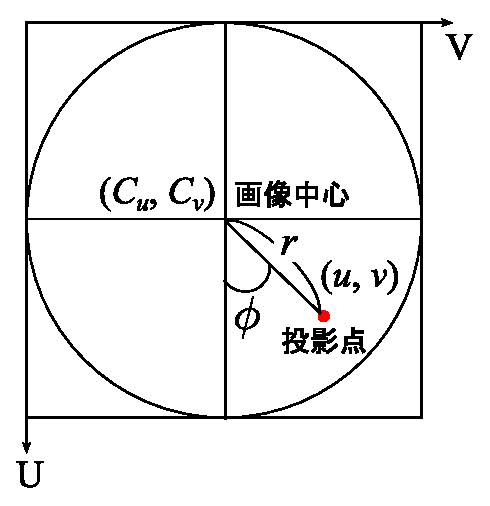
\includegraphics[width=5cm]{./chap3/eps/r2cucv.eps}
  \label{fig:pixel_kankei}}
%\vspace{10mm}
  \caption{���჌���Y�̓��ˌ��Ɠ��e�_�̊֌W}
  \label{fig:tourittai}
\end{figure}

\begin{table}[tb]
\begin{center}
\caption{�ˉe�������̉摜���S����̃s�N�Z������$r$�Ƙc�݃p�����[�^$k$�̊֌W}
\label{table:distortion_parameter}
\begin{tabular}{l c}\hline
�ˉe���� & $r$��$\theta$�̊֌W\\ \hline \hline
���ˉe���� & $r=k\sin{\theta}$ \\ 
�������ˉe���� & $r=k{\theta}$ \\
�����̊p�ˉe���� & $r=2k\sin{\frac{\theta}{2}}$ \\ \hline
\end{tabular}
\end{center}
\end{table}

\begin{equation}
\begin{bmatrix}
u\\
v
\end{bmatrix}
=
\begin{bmatrix}
r\cos\phi + C_u \\
r\sin\phi + C_v
\end{bmatrix} .
\label{eq:fisheye_uv}
\end{equation}

\begin{equation}
\phi = \cos^{-1}{\frac{x}{\sqrt{x^2 + y^2}}} = \sin^{-1}{\frac{y}{\sqrt{x^2 + y^2}}} .
\label{eq:fisheye_phi}
\end{equation}

\clearpage

���������ۂɂ̓����Y�쐬���ɐ������c�ݓ��̌�������C
�����Y�S�̂ɂ����ĕ\\ref{table:distortion_parameter}�̂悤��
�ˉe�������猈�肳���֌W���𖞂����Ă���킯�ł͂Ȃ��C�����Y���ɂ���Ă��قȂ�D
%�ɂ���đS�Ẵs�N�Z���Ɠ��ˌ��̊֌W�������ɕ\����킯�ł͂Ȃ��D
���̂��ߋ���摜�������Ɉ��������ꍇ�C�摜��̃s�N�Z���Ɠ��ˌ��̊֌W���������Y���ɎZ�o����K�v������D
�{�����ł́CScaramuzza��̎�@\cite{scaramuzza2006}�Ɠ��l�ɁC�摜���S����̃s�N�Z��������$r$�ł���s�N�Z��$(u, v)$�ƁC���ˌ��̃x�N�g��$(x, y, z)$�̊֌W����(\ref{eq:ocamcalib1})�C��(\ref{eq:uvr})�C��(\ref{eq:ocamcalib_k})�C��(\ref{eq:ocamcalib_g})�ŕ\���D
�܂����̊֌W���ɂ����āC$a_{i}$ $(i = 0,  1, 2, 3, 4)$��c�݃p�����[�^�C$r$�̊֐�$g(r)$��c�݊֐��ƌĂԂ��ƂƂ���D�L�����u���[�V�����ɂ���Ă��̘c�݃p�����[�^$a_{i}$ $(i = 0,  1, 2, 3, 4)$�����߂�D






%�����̊p�ˉe�����̑S�����჌���Y�̖͎��}��}\ref{fig:tourittai}�Ɏ����D
%�}\ref{fig:tourittai}����x���Cz���̓J�������W�n�̍��W���CU���CV���͓�����摜�̍��W����\���Ă���D
%�}\ref{fig:nyuusyakou}�͓��ˊp$\theta$�œ��˂������������Y�ŋ��܂��C�B���f�q�֓��e�����l�q��\���Ă���D�}\ref{fig:pixel_kankei}�͎B�e���ꂽ�摜��ł̉摜���S�ƁC���ړ_$(u, v)$�C�s�N�Z������$r$�̊֌W��\���Ă���D
%�\\ref{table:distortion_parameter}�Ɛ}\ref{fig:tourittai}���番����Ƃ���C�c�݃p�����[�^��m�邱�Ƃŋ���摜��̃s�N�Z���Ɠ��ˌ��̕����x�N�g�����Z�o���邱�Ƃ��”\�ł���D


\begin{equation}
\begin{bmatrix}
u-C_u\\
v-C_v\\
g(r)
\end{bmatrix}
=-k
\begin{bmatrix}
x\\
y\\
z
\end{bmatrix} .
\label{eq:ocamcalib1}
\end{equation}

\begin{equation}
r = \sqrt{(u-C_u)^2 + (v-C_v)^2} .
\label{eq:uvr}
\end{equation}

\begin{equation}
k = \sqrt{r^2 + \{g(r)\}^2} .
\label{eq:ocamcalib_k}
\end{equation}

\begin{equation}
g(r)=a_{0} + a_{1}r + a_{2}r^{2}+ a_{3}r^{3}+ a_{4}r^{4}\\
\label{eq:ocamcalib_g}
\end{equation}



\clearpage
%%%%%%%%%%%%%%%%%%%%%%%%%%%%%%%%%%%%%%%%%%%%%%%%%%%%%%%%%%%%%%%%%%%%%%%%%%%%%%%%%%%%%%%%%%%%%%%%%%%%%%%%%%%%%%%%%%%%%%%%%%%%%%%%%%%
\section{�J�����L�����u���[�V����}
\label{sec:calibration}
�O�q�̂Ƃ���C����J������ʂ��ĎB�e�����摜�̓����Y�ɂ��c�݂������Ă���D���̘c�݂�␳���邽�߂Ƀ����Y�ŗL�̃p�����[�^�𐄒肷��K�v������D
%�܂��C\ref{sec:rectified_coordinate}�߂ŏڂ����q�ׂ邪�C�{�����ł̓X�e���I�v�����s�����߂�2��̃J�����ŋ��ʂ������W�n��ݒ肷��D
�܂��C�e�J�����Ŏ擾�����摜�΂𕽍s�X�e���I�摜�΂ւƕϊ����邽�߂ɁC�n��ɐݒu���ꂽ�J�����Ԃ̈ʒu��p���𐄒肷��K�v������D
�����ŁC�{�߂ł́C�����Y�ŗL�̓����p�����[�^�ł���
�摜���S����јc�݃p�����[�^�̐����@��\ref{sec:internal_parameter}���C�O���p�����[�^�ł���J�����̈ʒu�p�����[�^��p���̉�]�p�����[�^�̐����@��\ref{sec:external_parameter}���ɂďq�ׂ�D

%\vspace{1cm}

%\begin{figure}[hbp]
%\begin{center}
%\includegraphics[width=10cm]{./chap3/tmp/parameter.eps}
%\caption{���肷��p�����[�^}
%\label{fig:parameter}
%\end{center}
%\end{figure}

%\clearpage
%\clearpage
%%%%%%%%%%%%%%%%%%%%%%%%%%%%%%%%%%%%%%%%%%%%%%%%
\subsection{�����p�����[�^�̐���}
\label{sec:internal_parameter}

�{�����ɂ����ĕK�v�ƂȂ鋛��J�����̓����p�����[�^�́C
\begin{itemize}
\item �摜���S�F$C_u$�C$C_v$
\item ���჌���Y�̘c�݃p�����[�^�F$a_{i}$ $(i = 0, 1, 2, 3, 4)$
\end{itemize}
�ł���D�Ȃ��摜���S�Ƃ̓����Y���S���猋���ʂւ̐����ƌ����ʂƂ̌�_���w���D\\%�����̐����@���ȉ��ŏq�ׂ�D
%\clearpage

%%%%%%%%%%%%%%%%%%%%%%%%%%%%%%%
%\subsubsection{�摜���S�̐���}



�{�����ł́C�����̓����p�����[�^�̐����Scaramuzza��̎�@���g�p����\cite{scaramuzza2006}�D
%����͈ȉ��̎菇�ōs���D
%�i�ȒP�Ɏ菇�������j
�B�e���u��ݒu�C�Œ肵����C�}\ref{fig:Ocam}�Ɏ����悤�Ɋi�q�p�^�[�����B�e�”\�͈͓��ňړ������Ȃ���l�X�Ȍ����p�x�ŎB�e����D�擾�����������̉摜����͉摜�Ƃ��C����J�����Ŏ擾�����摜�̉摜���S�̍��W($C_u$, $C_v$)�ƁC
�s�N�Z�����W�Ɠ��ˌ��̕����x�N�g���Ƃ��֌W�Â���c�݃p�����[�^$a_{i}$ $(i = 0, 1, 2, 3, 4)$�𐄒肷��D�{�����ɂ����Ă�10�����x�̎ʐ^����͂Ƃ����D

\vspace{1cm}

\begin{figure}[hbp]
\begin{center}
\includegraphics[width=11cm]{./chap3/tmp/ocamcalib.eps}
\caption{�����p�����[�^�̐���Ɏg�p������͉摜�̗�}
\label{fig:Ocam}
\end{center}
\end{figure}

%%%%%%%%%%%%%%%%%%%%%%%%%%%%%%%

%%%%%%%%%%%%%%%%%%%%%%%%%%%%%%%



%%%%%%%%%%%%%%%%%%%%%%%%%%%%%%%


\clearpage
%%%%%%%%%%%%%%%%%%%%%%%%%%%%%%%%%%%%%%%%%%%%%%%%%%%%%%%%%%%%%%%%%%%%%%%%%%%%%%%%%%%%%%%%%%%%%%%%%%%%%%%%%%%%%%%%%%%%%%%%%%%%%%%%%%%%%%%%%%%%%%%%%%%%%%%%%%
\subsection{�O���p�����[�^�̐���}
\label{subsec:external_parameter}

�{�����ɂ����ĕK�v�ƂȂ鋛��J�����̊O���p�����[�^�́C
\begin{itemize}
\item �J�����Ԃ̑��ΓI�Ȉʒu�p�����[�^�F�J�����ԋ���$d$�C���ʊp$\alpha$�C�Šp$\beta$
\item ��]�p�����[�^�F$\mathbf{R}$
\end{itemize}
�ł���D�����ŎZ�o�����]�p�����[�^�͊e�J�����̍��W�n�𕽍s���摜�֕ϊ����邽�߂̉�]�p�����[�^���w���D
�����̐����@���ȉ��ŏq�ׂ�D

%%%%%%%%%%%%%%%%%%%%%%%%%%%%%%%
\subsubsection{�ʒu�p�����[�^�̐���}
\label{ssec:position}
�{�����ł́C�g�p����B�e���u��GPS���j�b�g�𓋍ڂ���D����ɂ��C�B�e���u��ݒu�����ꏊ�̈ܓx�C�o�x�C�ȉ~�̍��Ƃ�����GPS�����擾���邱�Ƃ��”\�ł���D
GPS���j�b�g�ɂ���ē���e�J�����̈ʒu���𗘗p���C���N�e�B�t�@�C�h���W�n�ɂ�����J�����ԋ���$d$�𐄒肷��D
�܂�\ref{ssec:rotation}�ŏڍׂɏq�ׂ邪�C�e�J�����Ŏ擾�����摜�𕽍s���摜�ւƕϊ����邽�߂ɁC����̃J�������瑼���̃J�����ւ̕��ʊp$\alpha$�ƋŠp$\beta$���K�v�ł���D�������ʒu�p�����[�^�𗘗p���Đ��肷��D\\

�J�����ɓ��ڂ���GPS���j�b�g�ɂ��擾�����J�����ݒu�ʒu�̈ܓx��$lat$ [rad]�C�o�x��$lng$ [rad]�C�ȉ~�̍���$h$ [m]�Ƃ���D
�ȉ~�̍��Ƃ͒n����ȉ~�̂Ƌߎ������Ƃ��̑ȉ~�̂���̍����ł���D
�܂�GPS�ɂ���ē�������i$lat, lng, h$�j��p���ăJ�����ݒu�n�_�̍��W��ECEF�iEarth centered, earth fixed�j���W�n�ƌĂ΂����W�n�ŕ\������D
ECEF���W�n�͌��_��n���d�S�Ƃ��C$\rm Z^{ecef}$����n���̎��]���̖k�ɕ����C
$\rm X^{ecef}$����$\rm Z^{ecef}$���ɐ����Ŗ{���q�ߐ��̕����C$\rm Y^{ecef}$�����E��n�ł����̎��ƒ�������悤�ɒ�`�������W�n�ł���D
GPS����ECEF���W�n�Ƃ̊֌W��}\ref{fig:gps_ecef}�Ɏ����D
�܂��CGPS���$�ilat, lng, h�j$��ECEF���W�i$x^{ecef}, y^{ecef}, z^{ecef}$�j�ւƕϊ����邽�߂ɂ́C�n���̐ԓ����ϔ��a�ƝG�����Ƃ������萔���K�v�ł���D
�n���̌`���WGS84�����ȉ~�̂ƌĂ΂���]�ȉ~�̂Ƃ��ċߎ������Ƃ��C�ԓ����ϔ��a�ƝG�����͕\\ref{table:wgs84parameter}�̂悤�ɒ�߂��Ă���D\\

\begin{table}[b]
\begin{center}
\caption{WGS84�����ȉ~�̂̒萔}
\label{table:wgs84parameter}
\begin{tabular}{l c c}\hline
�p�����[�^ & �{�_�����ł̋L�� & �萔\\ \hline \hline
�ԓ��ʕ��ϔ��a �im�j & $a$ &6 378 137 \\ 
�G���� & $flat$ &1/298.257 223 563 \\ \hline
\end{tabular}
\end{center}
\end{table}

�\\ref{table:wgs84parameter}���g�p����ƁCWGS84�����ȉ~�̂̒Z���a$b$�Ɨ��S��$e$�͈ȉ��̎�(\ref{eq:WGS_b})�C��(\ref{eq:WGS_e})�ŕ\�����Ƃ��ł���D

\begin{equation}
b = a(1-flat)\\
\label{eq:WGS_b}
\end{equation}

\begin{equation}
e=\frac{\sqrt{a^2-b^2}}{a}\\
\label{eq:WGS_e}
\end{equation}


\begin{figure}[tp]
\begin{center}
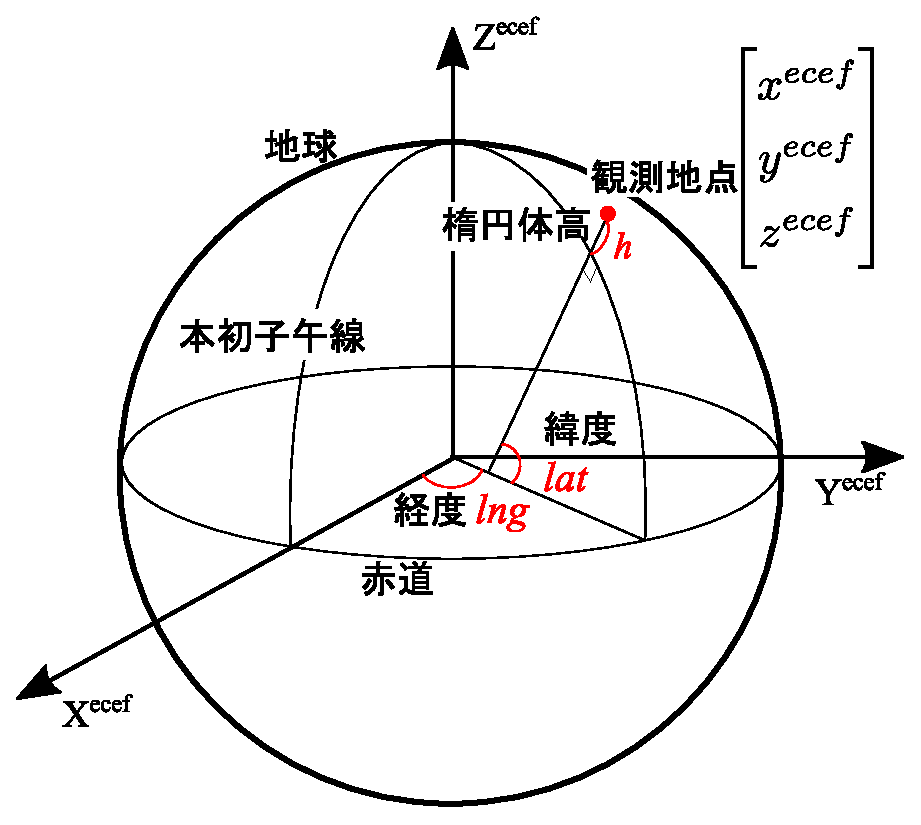
\includegraphics[width=8cm]{./chap3/eps/WGS84.eps}
\caption{GPS����ECEF���W�̊֌W}
\label{fig:gps_ecef}
\end{center}
\end{figure}

�\\ref{table:wgs84parameter}���̒萔�Ǝ�(\ref{eq:WGS_b})�C��(\ref{eq:WGS_e})��p���āC�ȉ��̎��ɂ����
GPS���$�ilat, lng, h�j$����ECEF���W$�ix^{ecef}, y^{ecef}, z^{ecef}�j$�ւƕϊ�����D\\


\begin{equation}
\begin{bmatrix}
x^{ecef}\\
y^{ecef}\\
z^{ecef}
\end{bmatrix}
=
\begin{bmatrix}
(N+h)\cos(lat)\cos(lng)\\
(N+h)\cos(lat)\sin(lng)\\
\{N(1-e^2)+h\}\sin(lat)
\end{bmatrix} .
\label{eq:GPS2ECEF}
\end{equation}

\begin{equation}
N = \frac{a}{\sqrt{1-e^2\sin^2(lat)}} .
\label{eq:WGS_N}
\end{equation}

\begin{figure}[tp]
\begin{center}
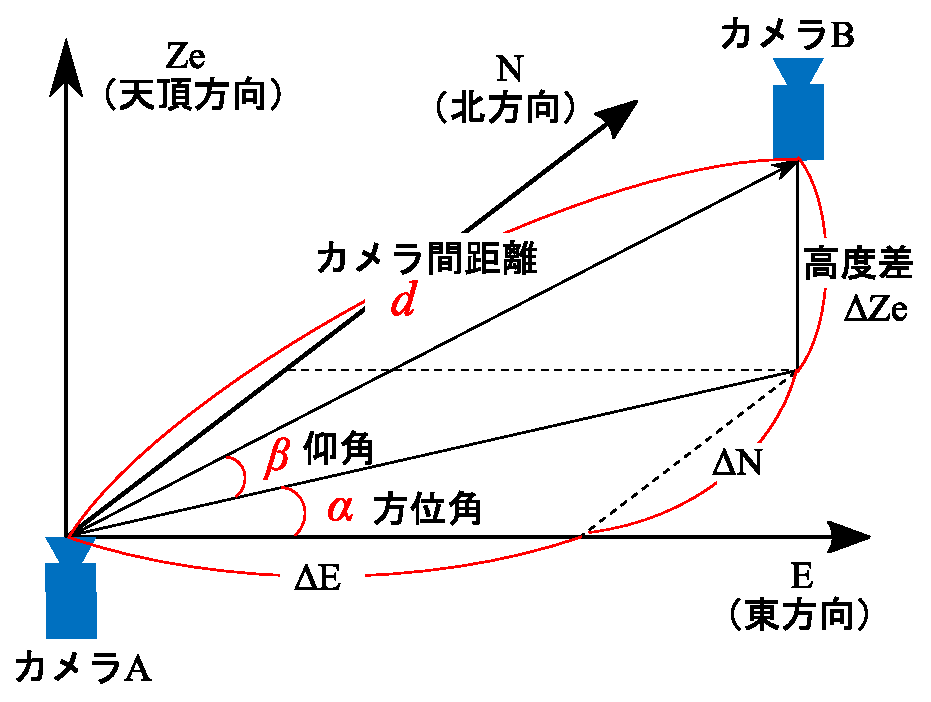
\includegraphics[width=8cm]{./chap3/eps/ENU.eps}
\caption{�J�����ԋ���$d$�C���ʊp$\alpha$�C�Šp$\beta$�̐���}
\label{fig:enu}
\end{center}
\end{figure}


���ɃJ����A�C�J����B��ECEF���W��p���āC�J�����ԋ���$d$�ƃJ��������J����B�ւ̕��ʊp$\alpha$�C�Šp$\beta$���Z�o����D
2��̃J������10 km�O��̈ʒu�ɐݒu����Ă��邽�߁C�n�\�𕽖ʂƋߎ�����D
�J����A�̐ݒu�ʒu�����_�Ƃ��C��������E���C�k������N���C�V��������Ze�����Ƃ���W�n��ݒ肷��D
���̂Ƃ��J����B��ENZe���W��$(\Delta E, \Delta N, \Delta Ze)$�Ƃ���ƁCENZe���W�n�Ƌ��߂�ʒu�p�����[�^$(d, \alpha, \beta)$�̊֌W�͐}\ref{fig:enu}�̂悤�ɂȂ�D
�܂��CENZe���W�n��ECEF���W�n��$\rm Z^{ecef}$���܂���$lng$ [rad]��]�������̂��C$\rm Y^{ecef}$���܂���$�i\pi / 2 - lat�j$ [rad]��]�����C�Ă�$\rm Z^{ecef}$���܂���$\pi / 2$ [rad]��]���������W�n�ł���D
�����ŁC�E����W�n��X���܂��CY���܂��CZ���܂���$\theta$ [rad]��]�������Ƃ��̍��W�ϊ��̍s������ꂼ��ȉ��̎�(\ref{eq:Rx})�C��(\ref{eq:Ry})�C��(\ref{eq:Rz})�̂悤�ɕ\���ƁC
$(\Delta E, \Delta N, \Delta Ze)$�͎�(\ref{eq:deltaEND})�ŎZ�o�����D



\begin{equation}
\mathbf{R}(X, \theta) =
\begin{pmatrix}
1 &0 &0 \\
0 &\cos(\theta) &\sin(\theta) \\
0 &-\sin(\theta) &\cos(\theta)
\end{pmatrix} .
\label{eq:Rx}
\end{equation}

\begin{equation}
\mathbf{R}(Y, \theta) =
\begin{pmatrix}
\cos(\theta) &0 &-\sin(\theta) \\
0 &1 &0 \\
\sin(\theta) &0 &\cos(\theta)
\end{pmatrix} .
\label{eq:Ry}
\end{equation}

\begin{equation}
\mathbf{R}(Z, \theta) =
\begin{pmatrix}
\cos(\theta) &\sin(\theta) &0 \\
-\sin(\theta) &\cos(\theta) &0 \\
0 &0 &1
\end{pmatrix} .
\label{eq:Rz}
\end{equation}

\begin{equation}
\begin{bmatrix}
\Delta E\\
\Delta N\\
\Delta Ze
\end{bmatrix}
=\mathbf{R}(Z^{ecef}, \pi /2)\mathbf{R}(Y^{ecef}, \pi /2-lat)\mathbf{R}(Z^{ecef}, lng)
\begin{bmatrix}
x^{ecef}_B - x^{ecef}_A \\
y^{ecef}_B - y^{ecef}_A \\
z^{ecef}_B - z^{ecef}_A 
\end{bmatrix} .
\label{eq:deltaEND}
\end{equation}


�}\ref{fig:enu}����C$(d, \alpha, \beta)$�͈ȏ�̎���p����$(\Delta E, \Delta N, \Delta Ze)$��p���Ď�(\ref{eq:abh})�ɂ���ĎZ�o�����D
�ȏ�̌v�Z�ɂ��C�J�����ɓ��ڂ���GPS�̏�񂩂�ʒu�p�����[�^���Z�o����D

\begin{equation}
\begin{bmatrix}
d\\
\alpha \\
\beta
\end{bmatrix}
=
\begin{bmatrix}
\sqrt{{\Delta E}^2 + {\Delta N}^2 + {\Delta Ze}^2} \\
\tan^{-1}({\Delta N}/{\Delta E}) \\
\tan^{-1}({\Delta Ze}/{\sqrt{{\Delta E}^2 + {\Delta N}^2}}) 
\end{bmatrix} .
\label{eq:abh}
\end{equation}







%%%%%%%%%%%%%%%%%%%%%%%%%%%%%%%

%\clearpage
%%%%%%%%%%%%%%%%%%%%%%%%%%%%%%%
\vspace{1cm}
\subsubsection{�J�����p�����킹�̂��߂̉�]�p�����[�^����}
\label{ssec:rotation}
%%%%%%%%%%%%%%%%%%%%%%%%%%%%%%%
\ref{ssec:position}�ڂɂĊe�J�����̈ʒu�p�����[�^�̎擾�ɂ‚��ďq�ׂ����CGPS���j�b�g���瓾������ł͊e�ʒu�ɂ�����J�����̎p�������ʂ��邱�Ƃ͂ł��Ȃ��D
�J�����̎p�������ʂ����N�e�B�t�@�C�h���W�n�ɂĊe�J�����𕽍s�X�e���I�̊֌W�ɕϊ����邽�߁C�ȉ��̎�@�ɂ���]�p�����[�^�𐄒肷��D
�{�����ł́C���̈ʒu�𗘗p���邱�Ƃʼn�]�p�����[�^�𐄒肷��D
�B�e�����摜���Ŗ��m�Ɋm�F�ł���N�‚̍P�����蓮�Ŏw�肵�C�摜���̐��ւ̕����x�N�g���ƁC���N�e�B�t�@�C�h���W�n�ɂ����鐯�ւ̕����x�N�g�����r���邱�Ƃɂ���Đ��肷��D\\
%�{�����ł͉摜���Ŗ��m�Ɋm�F�ł���N�‚̍P�����蓮�Ŏw�肷��D



�摜���擾�����ۂ̃J�������W�n�ɂ�����C�ϑ��n�_����${\it N}$�‚̊e���Ɍ����������̒P�ʃx�N�g�������ꂼ��$\mathbf{n_1}$�C$\mathbf{n_2}$...$\mathbf{n_{\it i}}$�Ƃ��C
���N�e�B�t�@�C�h���W�n�ł̊ϑ��n�_����${\it N}$�‚̊e���֌����������̒P�ʃx�N�g�������ꂼ��$\mathbf{m_1}$�C$\mathbf{m_2}$...$\mathbf{m_{\it i}}$�Ƃ���i������$i = 1, 2, ..., N$�j�D
%$(x_1, y_1, z_1)$�C$(x_2, y_2, z_2)$...$(x_i, y_i, z_i)$�i������$i = 1, 2, ..., N$�j�Ƃ���D
%�܂��C���N�e�B�t�@�C�h���W�n�ł̊ϑ��n�_����N�‚̊e���֌����������̒P�ʃx�N�g�������ꂼ��$(X_1, Y_1, Z_1)$�C$(X_2, Y_2, Z_2)$...$(X_i, Y_i, Z_i)$�i������$i = 1, 2, ..., N$�j�Ƃ���D
�܂��C$\mathbf{n_{\it i}} = (x_i, y_i, z_i)^T$�C$\mathbf{m_{\it i}} = (X_i, Y_i, Z_i)^T$�ƕ\���D
�J�����p���Ɛ��̕����x�N�g����\�����}��}\ref{fig:vector_direction}�Ɏ����D
�}\ref{fig:vector_direction}�ɂ�����ԐF�̃J�����p�������ۂ̃J�����p���C�F�̃J�����p�������N�e�B�t�@�C�h���W�n�ł̃J�����p���Ƃ���D
�_���̖��Ŏ����ꂽ���������ꂼ��̎p���ł̌��������ł���D�����Ń��N�e�B�t�@�C�h���W�n����J�������W�n�ւ̉�]�s���$\mathbf{R}$�Ƃ���ƁC
��(\ref{eq:nRm})�����藧�D
\begin{eqnarray}
\mathbf{n_{\it i}}=\mathbf{Rm_{\it i}}
\label{eq:nRm}
\end{eqnarray}

��(\ref{eq:nRm})���C�x�N�g��$\mathbf{n_{\it i}}�C\mathbf{m_{\it i}}$�����߂�Ή�]�p�����[�^�𐄒肷�邱�Ƃ��ł���D

\clearpage

%\vspace{1cm}
\begin{figure}[tb]
\begin{center}
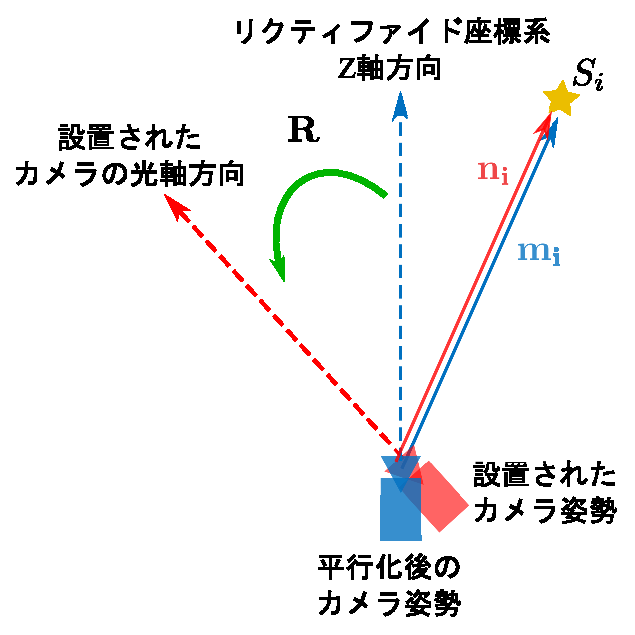
\includegraphics[width=7cm]{./chap3/eps/Camera2star.eps}
\caption{�J�����p���Ɛ��ւ̕����x�N�g��}
\label{fig:vector_direction}
\end{center}
\end{figure}


%\clearpage
%%%%%%%%%%%%%%%%%%%%%%%%%%%%%%
�ϑ��n�_����{\it i}�Ԗڂ̐�$S_i$�֌����������x�N�g��$\mathbf{n_{\it i}}$�͎�(\ref{eq:ocamcalib1})�C��(\ref{eq:ocamcalib_k})���Z�o�”\�ł���D
$S_i$�̉摜���ł̈ʒu��$(u_i, v_i)$�C�摜���S����̉摜���$S_i$�܂ł̋�����$r_i$�C�g�p���郌���Y�̘c�݊֐���$g(r)$�Ƃ���ƁC
$\mathbf{n_{\it i}}$�͎�(\ref{eq:ni})�ɂ���ċ��߂���D

\begin{eqnarray}
\mathbf{n_{\it i}}=
\left[\begin{array}{cc}x_i \\ y_i \\ z_i \end{array}\right]={\frac{1}{\sqrt{r_i^2 + g(r_i)^2}}}\left[\begin{array}{cc}u_i-C_u \\ v_i-C_v \\ g(r_i)  \end{array}\right]
\label{eq:ni}
\end{eqnarray}

�Ȃ��C�c�݊֐�$g(r)$���̘c�݃p�����[�^$a_{i}$ $(i = 0, 1, 2, 3, 4)$��\ref{sec:internal_parameter}���ŏq�ׂ��Ƃ���Scaramuzza��̎�@�ɂ��擾�”\�ł���D\\

\clearpage
%%%%%%%%%%%%%%%%%%%%%%%%%%%%%%


���Ƀ��N�e�B�t�@�C�h���W�n�ɂ�����$S_i$�ւ̕����̒P�ʃx�N�g��$\mathbf{m}_i$�����߂�D
���̂��߂ɂ́C�B�e���������ɂ�����$S_i$�̈ʒu��m��K�v�����邪�C
�C�ӂ̎����C�ʒu�C�����Ŋϑ������Ƃ��̑S�Ă̐��̈ʒu�͌����ɒm�邱�Ƃ��ł���D�܂��C���̈ʒu���v���l�^���E���`���ŕ\�����C�e�Ղɒm�邱�Ƃ��ł���悤�ɂ����\�t�g�E�F�A���������݂���D
�{�����ł́C���̒���1�‚ł���Toxsoft�Ђ��J������Stella Theater Lite���g�p����D�{�����ɂĎg�p���鐯�̒n�}�iStella Theater Lite�j��}\ref{fig:star_map}�Ɏ����D\\

\vspace{1cm}
\begin{figure}[hb]
\begin{center}
\includegraphics[width=9cm]{./chap3/tmp/StellaTheaterLite2.eps}
\caption{���̒n�}�iStella Theater Lite�j}
\label{fig:star_map}
\end{center}
\end{figure}

\clearpage

���̒n�}�֓��͂Ƃ���GPS���j�b�g�ɂ���Ď擾����ϑ��n�_�̈ܓx�C�o�x�C�B�e������^���邱�ƂŁC�ϑ��n�_���炱�̒n�}��̔C�ӂ̐��ւ̕��ʊp$Az$ [deg]�C�Šp$El$ [deg]���擾���邱�Ƃ��ł���D
�������C���̕��ʊp�͓삩�瓌�Ɍ����������֐��C�Šp�͒n�\����V���֌����������𐳂Ƃ��Ď擾�����D
�����ŁC�O�q��ENZe���W�n�ɂ����Đ}\ref{fig:world_vector}�Ɏ����悤��$(\theta_i�C\phi_i)$���`����Ƃ��C
$(\theta_i�C\phi_i)$�͎�(\ref{eq:AzEl})�ɂ���ĕ\����C
$(\theta_i�C\phi_i)$��p����ENZe���W�n�ɂ�����$S_i$�̕����̒P�ʃx�N�g�� $(E_i, N_i, Ze_i)^T$�͈ȉ��̎�(\ref{eq:xyz})�ɂ��Z�o�����D

\begin{equation}
\begin{bmatrix}
\theta_i\\
\phi_i
\end{bmatrix}
=
\begin{bmatrix}
\pi / 2 - El\\
Az - \pi / 2
\end{bmatrix} .
\label{eq:AzEl}
\end{equation}

\begin{eqnarray}
\left[\begin{array}{cc}E_i \\ N_i \\ Ze_i \end{array}\right]=\left[\begin{array}{cc}\sin\theta_i\cos\phi_i \\ \sin\theta_i\sin\phi_i \\ \cos\theta_i \end{array}\right]
\label{eq:xyz}
\end{eqnarray}

\begin{figure}[hbp]
\begin{center}
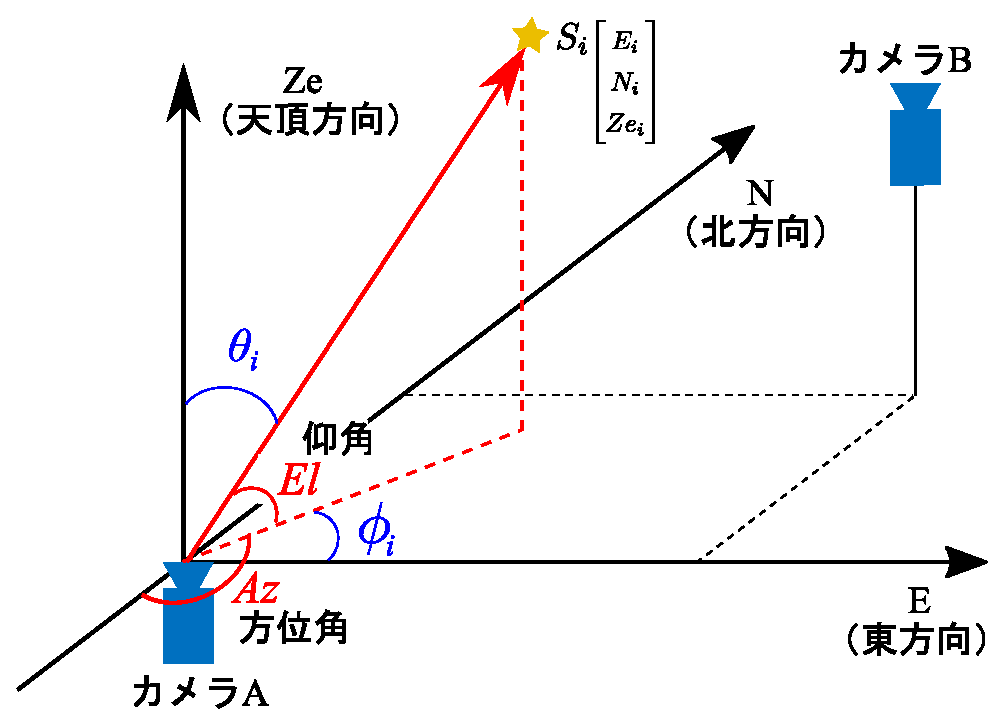
\includegraphics[width=9cm]{./chap3/eps/END2star.eps}
\caption{���E���W�n�ɂ����鐯�ւ̕����x�N�g���̎Z�o}
\label{fig:world_vector}
\end{center}
\end{figure}

\clearpage


���E���W�n�ɂ����鐯�̕����x�N�g�������N�e�B�t�@�C�h���W�n�ɂ���������x�N�g���֕ϊ����邽�߂ɁC\ref{ssec:position}�ڂ�GPS�̈ʒu��񂩂�Z�o�����J�����Ԃ̕��ʊp$\alpha$�ƋŠp$\beta$���g�p����D
���N�e�B�t�@�C�h���W�n�ɂ����鐯�̕����x�N�g���̎Z�o��}\ref{fig:ricthi_vector}�Ɏ����D�}����X���CY���CZ���̓��N�e�B�t�@�C�h���W�n�̍��W���ł���D
�}\ref{fig:ricthi_vector}���番����悤�ɁCENZe���W�n�����N�e�B�t�@�C�h���W�n�ւƕϊ����邽�߂ɂ�Ze���܂���$\alpha$��]������CN���܂���-$\beta$��]����΂悢�D
�����Ń��N�e�B�t�@�C�h���W�n�ɂ�����$S_i$�Ɍ����������̒P�ʃx�N�g��$\mathbf{m_{\it i}}$�́C��(\ref{eq:Ry})�Ǝ�(\ref{eq:Rz})�Œ�`������]�s��ƁC��(\ref{eq:xyz})�ŎZ�o����ENZe���W�n�ɂ�����$S_i$�̕����̒P�ʃx�N�g�� $(E_i, N_i, Ze_i)^T$��p����
�ȉ��̎�(\ref{eq:ricthi_vector})�ɂ���ĎZ�o�����D

\begin{equation}
\mathbf{m_{\it i}}=
\begin{bmatrix}
X_i\\
Y_i\\
Z_i
\end{bmatrix}
=\mathbf{R}(N, -\beta)\mathbf{R}(D, \alpha)
\begin{bmatrix}
E_i\\
N_i\\
Ze_i
\end{bmatrix}
\label{eq:ricthi_vector}
\end{equation}
%\clearpage

\vspace{2cm}


\begin{figure}[hbp]
\begin{center}
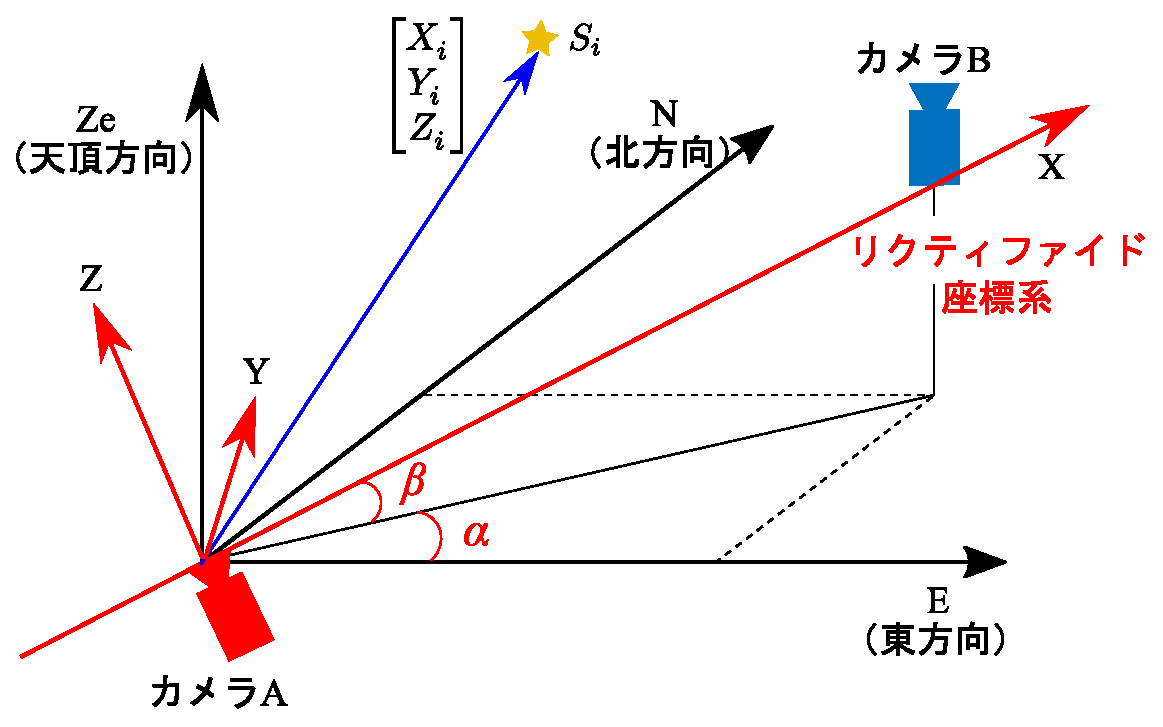
\includegraphics[width=11cm]{./chap3/eps/ricthi_vector.eps}
\caption{���N�e�B�t�@�C�h���W�n�ɂ����鐯�ւ̕����x�N�g���̎Z�o}
\label{fig:ricthi_vector}
\end{center}
\end{figure}

\clearpage


�����ŁC���N�e�B�t�@�C�h���W�n����J�������W�n�ւ̉�]�s��$\mathbf{R}$��$N$�‚̐��S�Ăɂ����Ď�(\ref{eq:nRm})�𖞂����s��ł���D
����āC���N�e�B�t�@�C�h���W�n�ɂ�����$S_i$�̕����x�N�g��$\mathbf{m_{\it i}}$�ƁC�J�������W�n�ɂ�����$S_i$�̕����x�N�g��$\mathbf{n_{\it i}}$����C��]�s��$\mathbf{R}$��p�����Ƃ��̌덷$\|\mathbf{n}_i - \mathbf{R}\mathbf{m}_i\|^2$�̑��a���ŏ��ƂȂ�悤��
��]�s��$\mathbf{R}$�����߂�D
�{�����ł͎�(\ref{eq:Restimate})�Ŏ����悤�ɓ��ْl������p���āC�J����A�C�J����B�̏ꍇ���ꂼ��ɂ�����$\mathbf{R}$�𐄒肷��D

\begin{equation}
\begin{split}
\min\sum_{i=1}^\mathbf{n} \|\mathbf{n}_i - \mathbf{R}\mathbf{m}_i\|^2 \\
= \min\|\mathbf{N} - \mathbf{RM} \|^2 \\
������ \mathbf{N} = (\mathbf{n}_1, \mathbf{n}_2, ..., \mathbf{n}_n), \mathbf{M} = (\mathbf{m}_1, \mathbf{m}_2, ..., \mathbf{m}_n)\\
\\
������\|\mathbf{N} - \mathbf{RM} \|^2\\
= tr((\mathbf{N}-\mathbf{RM})^T(\mathbf{N}-\mathbf{RM}))\\
=tr(\mathbf{N}^T\mathbf{N})+tr(\mathbf{M}^T\mathbf{M})-2tr(\mathbf{N}^T\mathbf{RM})�@����\\
\min\|\mathbf{N} - \mathbf{RM} \|^2 ���@\max(tr(\mathbf{N}^T\mathbf{RM}))�ƂȂ�\\
\\
\mathbf{MN}^T = \mathbf{U\Sigma V}^T�Ƃ����\\
tr(\mathbf{N}^T\mathbf{RM}) = tr(\mathbf{RMN}^T)\\
=tr(\mathbf{RU\Sigma V}^T)\\
=tr(\mathbf{V}^T\mathbf{RU\Sigma V}) \leq tr(\Sigma)�@���\\
\mathbf{V}^T\mathbf{RU} = \mathbf{I}_3�@�̂Ƃ��@tr(\mathbf{N}^T\mathbf{RM})�� \max �ƂȂ�\\
����ā@\mathbf{R} = \mathbf{VU}^T
\end{split}
\label{eq:Restimate}
\end{equation}


\textcolor{red}{������}

%\begin{equation}
% \mathbf{R}=\argmin_{R}E
%\label{eq:saisyouR}
%\end{equation}





\clearpage
%%%%%%%%%%%%%%%%%%%%%%%%%%%%%%%%%%%%%%%%%%%%%%%%%%%%%%%%%%%%%%%%%%%%%%%%%%%%%%%%%%%%%%%%%%%%%%%%%%%%%%%%%%%%%%%%%%%%%%%%%%%%%%%%%%%
\section{���N�e�B�t�@�C�h���W�n�摜�ւ̕ϊ�}
\label{sec:translation}

�{�߂ł́C\ref{sec:calibration}�߂ɂĐ��肵���p�����[�^����ɁC�摜��
\ref{sec:rectified}�߂Œ�`�������N�e�B�t�@�C�h���W�n�ɏ]�����s���摜�ւƕϊ������@�ɂ‚��ďq�ׂ�D
�摜�̕ϊ��ɂ́C\ref{sec:external_parameter}���ɂĐ��肵����]�s��$\mathbf{R}$��p����D
�ϊ���̉摜��̔C�ӂ̓_��$(U, V)$�C����ɑΉ�����ϊ��O�̉摜��̓_��$(u, v)$�Ƃ���D
\ref{sec:internal_parameter}���ɂĐ��肵���摜���S$(C_u, C_v)$�C�c�݊֐�$g(r)$���g�p���C
��(\ref{eq:ocamcalib1})--��(\ref{eq:ocamcalib_k})����C$(u, v)$�ɑΉ�����3���������x�N�g��$\mathbf{n}$����(\ref{eq:n_vector})�̂悤�ɎZ�o�”\�ł���D\\

\begin{equation}
\mathbf{n}=\frac{1}{\sqrt{r^2 +g(r)^2}}
\begin{bmatrix}
u-C_u\\
v-C_v\\
g(r)
\end{bmatrix}
=
\begin{bmatrix}
x(u,v)\\
y(u,v)\\
z(u,v)
\end{bmatrix}
\label{eq:n_vector}
\end{equation}


�����ŁC��]�s��$\mathbf{R}$�̓��N�e�B�t�@�C�h���W�n����J�������W�n�֕ϊ�����s��ł��邽�߁C
��(\ref{eq:nRm})�����藧�D
����ĉ�]�s��$\mathbf{R}$�̋t�s��$\mathbf{R}^{-1}$����(\ref{eq:rotation_matrix_Inver})�ŕ\���ƁC
$(U, V)$�ɑΉ�����3���������x�N�g��$\mathbf{m}$�͎�(\ref{eq:m_vector})�ɂ�蓾���C
��(\ref{eq:m_vector})����ɍ��W�\��$(\theta�C\phi)$�͎�(\ref{eq:theta_phi})�ɂ��C$\mathbf{n}$�̊֐��Ƃ��ĕ\����D\\

\begin{equation}
\mathbf{R}^{-1}=
\begin{bmatrix}
r_{11} &r_{12} &r_{13}\\
r_{21} &r_{22} &r_{23}\\
r_{31} &r_{32} &r_{33}
\end{bmatrix}
=
\begin{bmatrix}
\mathbf{r}_{1}\\
\mathbf{r}_{2}\\
\mathbf{r}_{3}
\end{bmatrix}
�C\mathbf{r}_{k}=
\begin{bmatrix}
r_{k1} &r_{k2} &r_{k3}
\end{bmatrix}
�ik=1,2,3�j
\label{eq:rotation_matrix_Inver}
\end{equation}

\begin{equation}
\mathbf{m}=
\begin{bmatrix}
\sin\theta\cos\phi\\
\sin\theta\sin\phi\\
\cos\theta
\end{bmatrix}
=\mathbf{R}^{-1}\mathbf{n}=
\begin{bmatrix}
\mathbf{r}_{1}\mathbf{n}\\
\mathbf{r}_{2}\mathbf{n}\\
\mathbf{r}_{3}\mathbf{n}
\end{bmatrix}
\label{eq:m_vector}
\end{equation}

%\begin{equation}
%\theta= \arccos(\mathbf{r}_{3}\mathbf{n})= f(\mathbf{n}), \phi=\arctan(\frac{\mathbf{r}_{2}\mathbf{n}}{\mathbf{r}_{1}\mathbf{n}})=g(\mathbf{n})
%\label{eq:theta_phi}
%\end{equation}

\begin{equation}
\begin{bmatrix}
\theta\\
\phi
\end{bmatrix}
=
\begin{bmatrix}
\cos^{-1}(\mathbf{r}_{3}\mathbf{n})\\
\tan^{-1}({\mathbf{r}_{2}\mathbf{n}}/{\mathbf{r}_{1}\mathbf{n}})
\end{bmatrix}
=
\begin{bmatrix}
h(\mathbf{n})\\
i(\mathbf{n})
\end{bmatrix}
\label{eq:theta_phi}
\end{equation}


�܂��C�g�p����J�����̓L�����u���[�V�������������Ă��邽�߁C
�����̓��ˊp$\theta$�Ɠ��e�_����摜���S�܂ł̋���$r'$�Ƃ̊֌W�͊��m�ł���D
�����$r'$����(\ref{eq:theta_r})�̂悤��$\theta$�ŕ\�����Ƃ��ł���D\\

\begin{equation}
r' = j(\theta)
\label{eq:theta_r}
\end{equation}


\clearpage
��(\ref{eq:fisheye_uv})�C��(\ref{eq:theta_r})����C$(U, V)$�͎�(\ref{eq:UV_uv})�ɂ��$(\theta�C\phi)$�̊֐��ŕ\����D\\

\begin{equation}
\begin{bmatrix}
U\\
V
\end{bmatrix}
=
\begin{bmatrix}
C_u+r'\cos\phi\\
C_v+r'\sin\phi
\end{bmatrix}
=
\begin{bmatrix}
s(\theta,\phi)\\
t(\theta,\phi)
\end{bmatrix}
\label{eq:UV_uv}
\end{equation}

�ȏ�̎�(\ref{eq:n_vector})--��(\ref{eq:UV_uv})����C�ϊ���̓_�ϊ���̓_$(U, V)$�ƁC�ϊ��O�̓_$(u, v)$�Ƃ̑Ή����Z�o�ł��邽�߁C
���N�e�B�t�@�C�h���W�n�ɏ]���摜���擾���邱�Ƃ��”\�ł���D\\

���N�e�B�t�@�C�h���W�n�ɏ]���摜�֕ϊ��O�̉摜�̗��}\ref{fig:trans_in}�C�ϊ���̉摜�̗��}\ref{fig:trans_out}�Ɏ����D
�J����A�C�J����B�ŎB�e���ꂽ�摜���̃I�[�����`���ڎ��ł��ꂼ���r����ƁC
�ϊ��O�̐}\ref{fig:trans_in}�ɂ����Ă݂͂͌��Ɋp�x���قȂ��Ă������C
�ϊ���̐}\ref{fig:trans_out}�ɂ����Ă�2���̉摜���̃I�[�����̌�������v���Ă��邱�Ƃ��m�F�ł���D

\clearpage

\begin{figure}[htb]
  \centering
  \subfigure[�J����A]{
    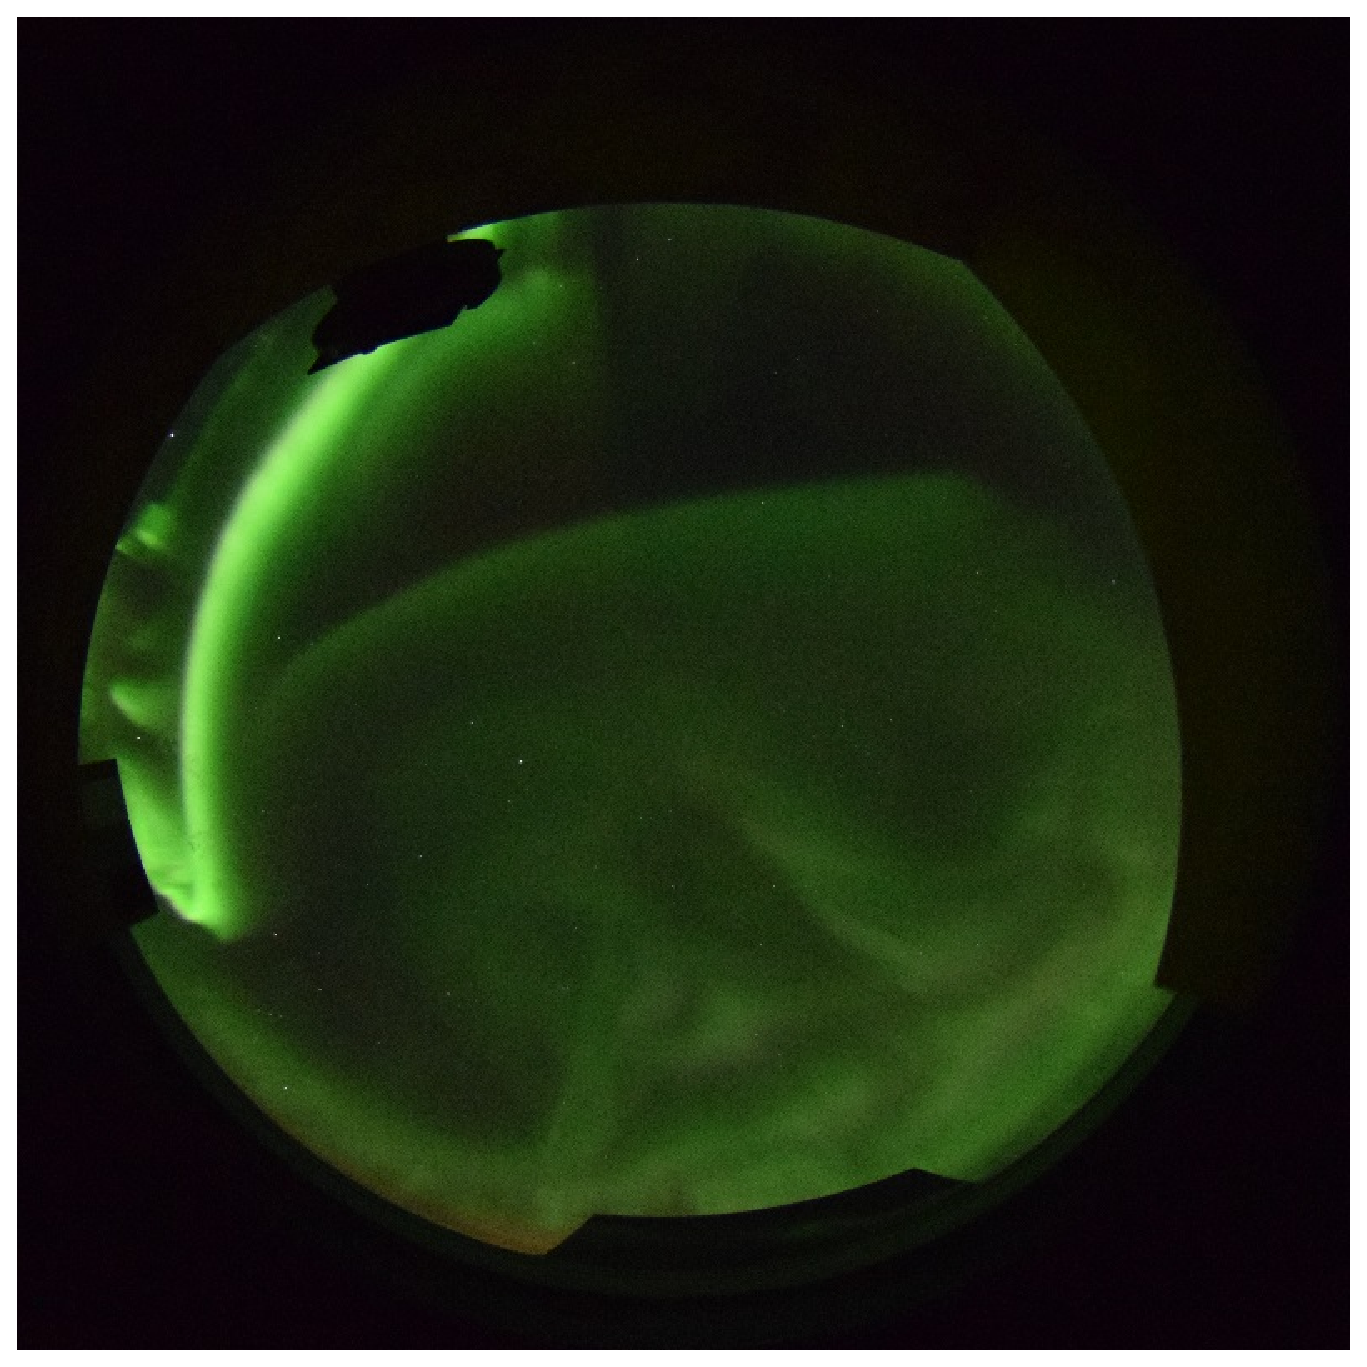
\includegraphics[width=5cm]{./chap3/eps/019_ori_L.eps}
  \label{fig:trans_in1}}
  \subfigure[�J����B]{
    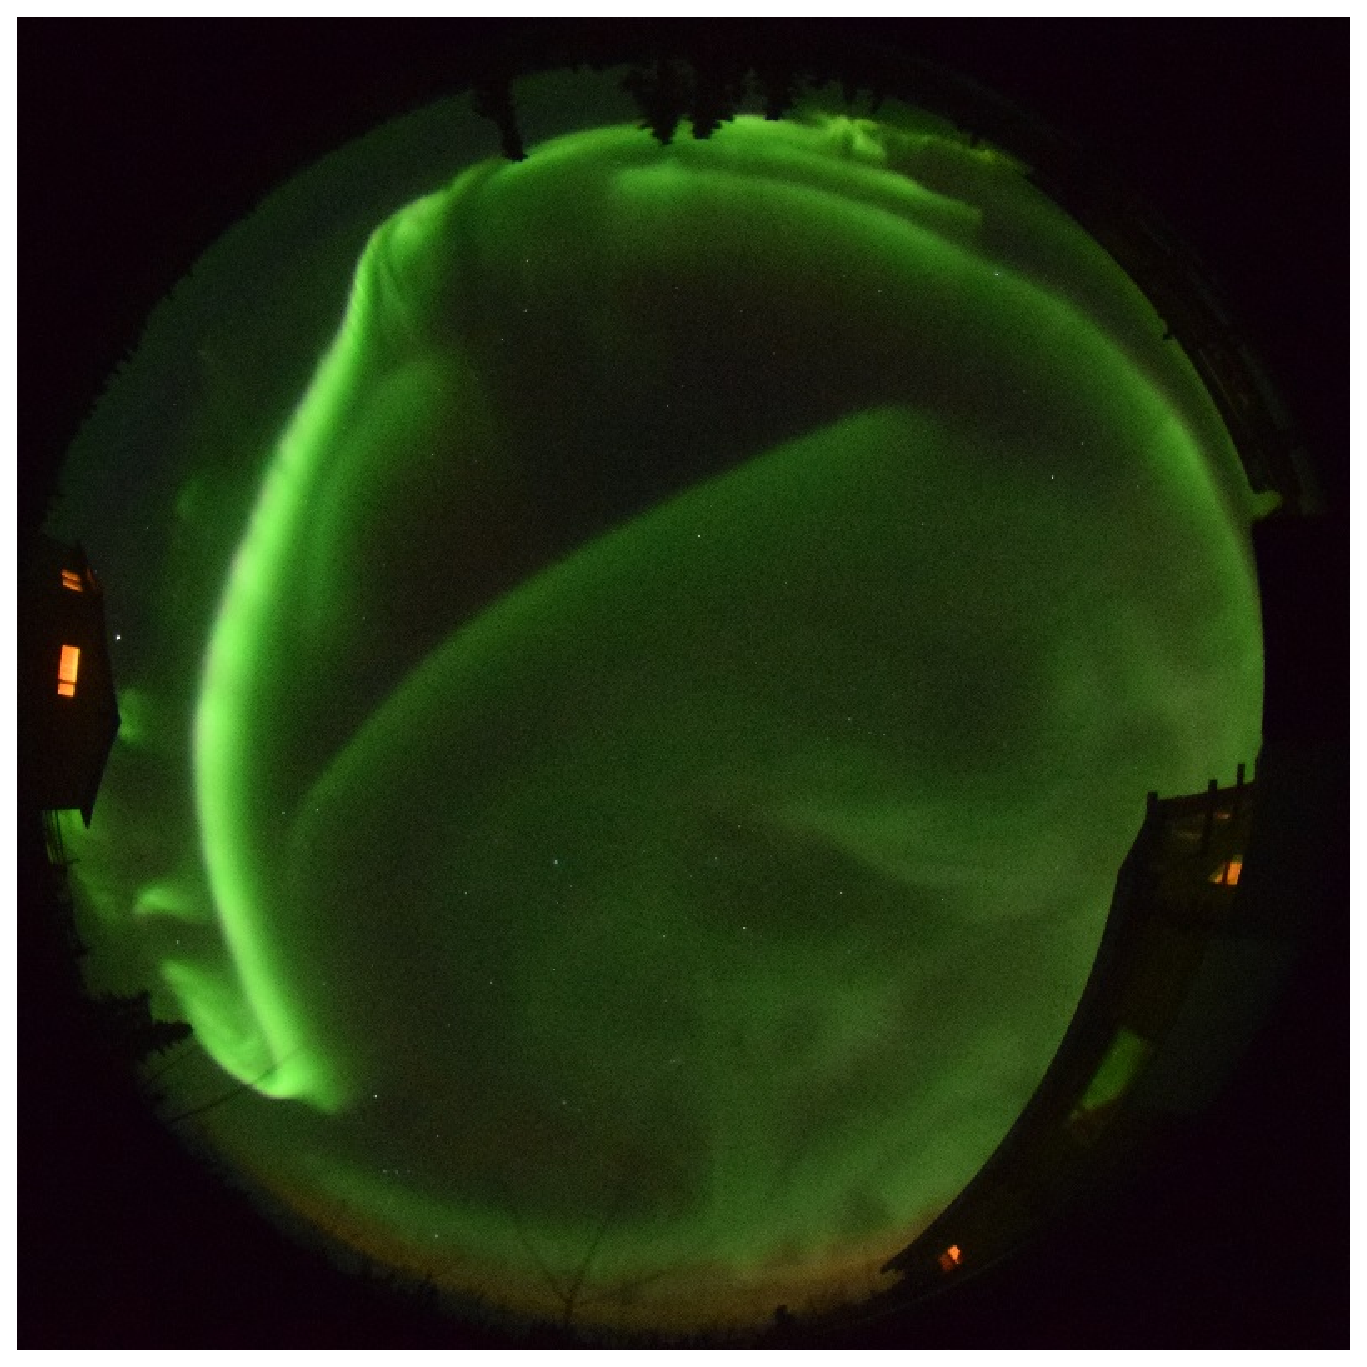
\includegraphics[width=5cm]{./chap3/eps/019_ori_R.eps}
  \label{fig:trans_in2}}
  \caption{���N�e�B�t�@�C�h���W�n�ւ̕ϊ��O�摜}
  \label{fig:trans_in}
\end{figure}


\begin{figure}[htb]
  \centering
  \subfigure[�J����A]{
    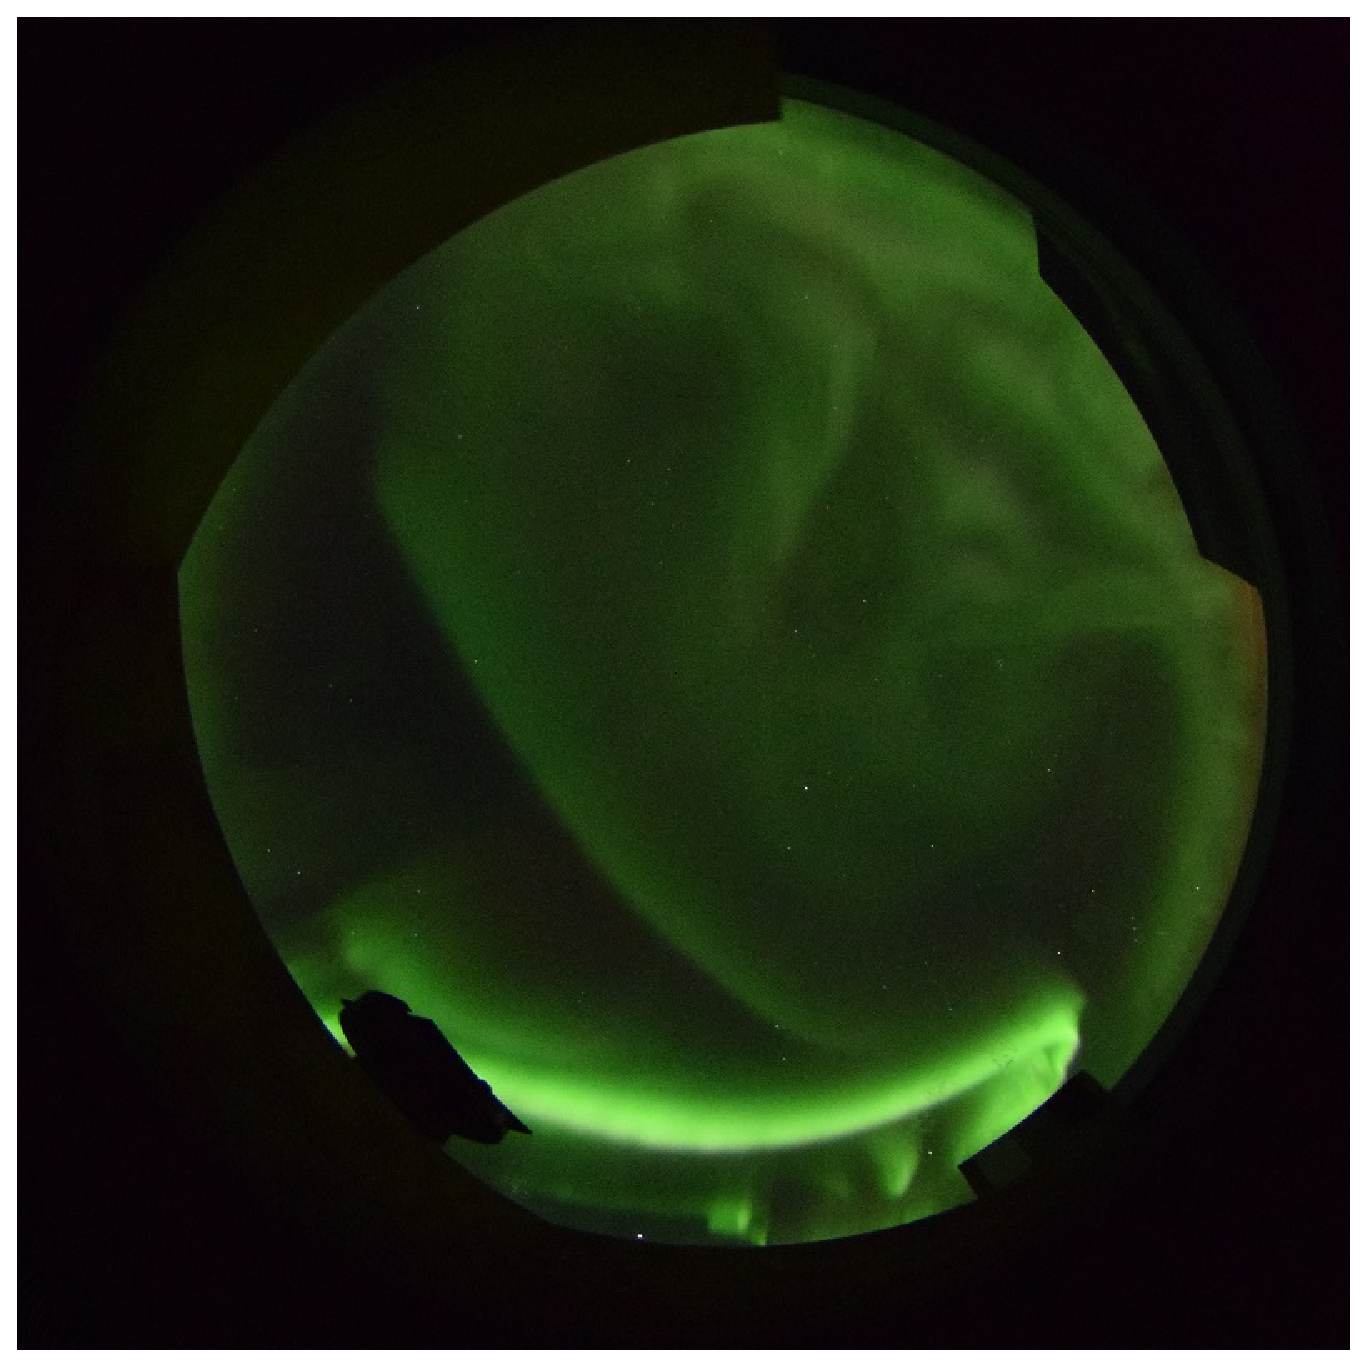
\includegraphics[width=5cm]{./chap3/eps/019_trans_L.eps}
  \label{fig:trans_out1}}
  \subfigure[�J����B]{
    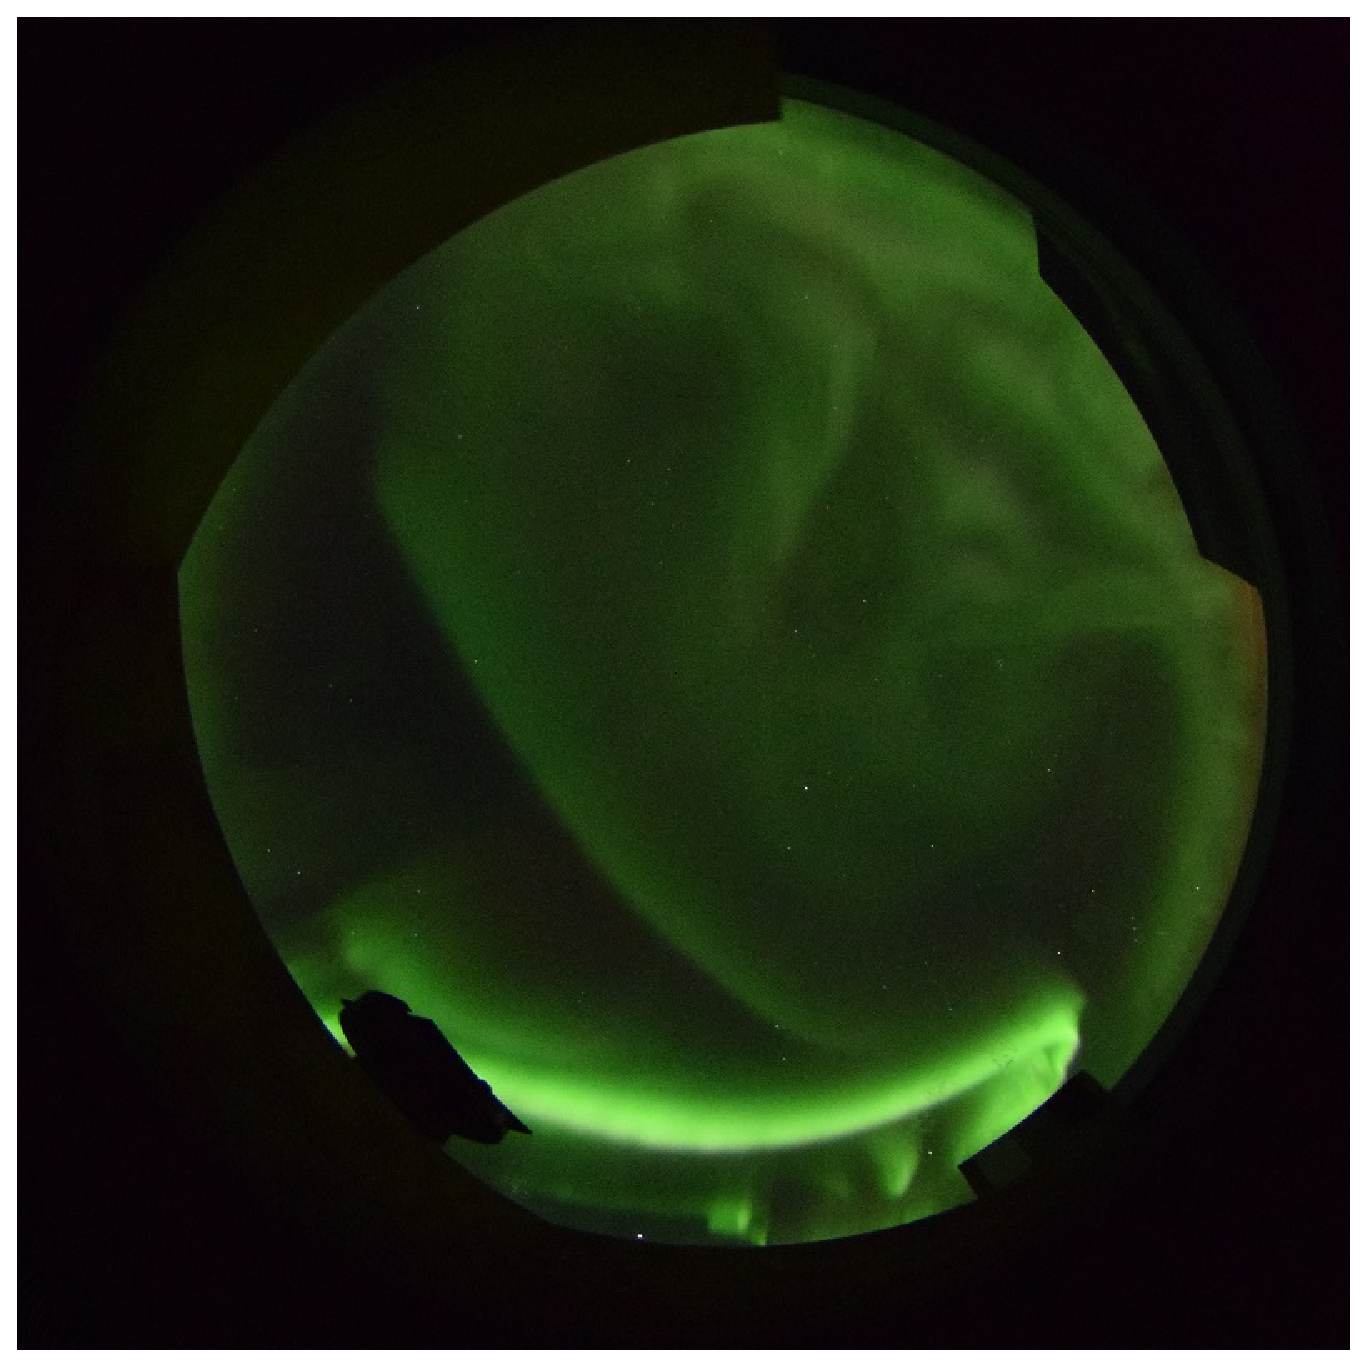
\includegraphics[width=5cm]{./chap3/eps/019_trans_L.eps}
  \label{fig:trans_out2}}
  \caption{���N�e�B�t�@�C�h���W�n�ւ̕ϊ���摜}
  \label{fig:trans_out}
\end{figure}

\clearpage

%�i�摜�����ւ��H�j
%%%%%%%%%%%%%%%%%%%%%%%%%%%%%%%%%%%%%%%%%%%%%%%%%%%%%%%%%%%%%%%%%%%%%%%%%%%%%%%%%%%%%%%%%%%%%%%%%%%%%%%%%%%%%%%%%%%%%%%%%%%%%%%%%%%
\section{����摜���瓧�����e�摜�ւ̕ϊ�}
\label{sec:undistortion}

����J�����ɂ��擾����摜�́C���჌���Y�̐����ɂ��c�݂�L����D�{�߂ł͎擾�摜���狛�჌���Y�ɂ��c�݂��������������e�ˉe�摜�֕ϊ�����D
�{�����Ŏg�p���鋛�჌���Y�̘c�݂�\ref{sec:internal_parameter}���Ő��肵���c�݊֐��Ɋ�Â��Ă���D
���ˌ��Ɖ摜��̓��e�_�̊֌W�̓L�����u���[�V�����ɂ���Ď�(\ref{eq:theta_r})�̂悤�Ɋ��m�ł���Ƃ���D\\

����摜���瓧�����e�摜�ւ̕ϊ��̗l�q��}\ref{fig:fisheye_ray}�C�}\ref{fig:hoseimen}�Ɏ����D
�}\ref{fig:fisheye_ray}�C�}\ref{fig:hoseimen}�͓������e�摜���ʂ��œ_����$Z_v$�̋����ɂ��邫�C
�������e�摜��̓��e�_�Ƌ���摜��̓��e�_���֌W�t���Ă���}�ł���D
����摜��̔C�ӂ̓_$(x_f, y_f)$���������e�摜���$(x_p, y_p)$�ƂȂ�Ƃ���D\\

\begin{figure}[b]
\begin{center}
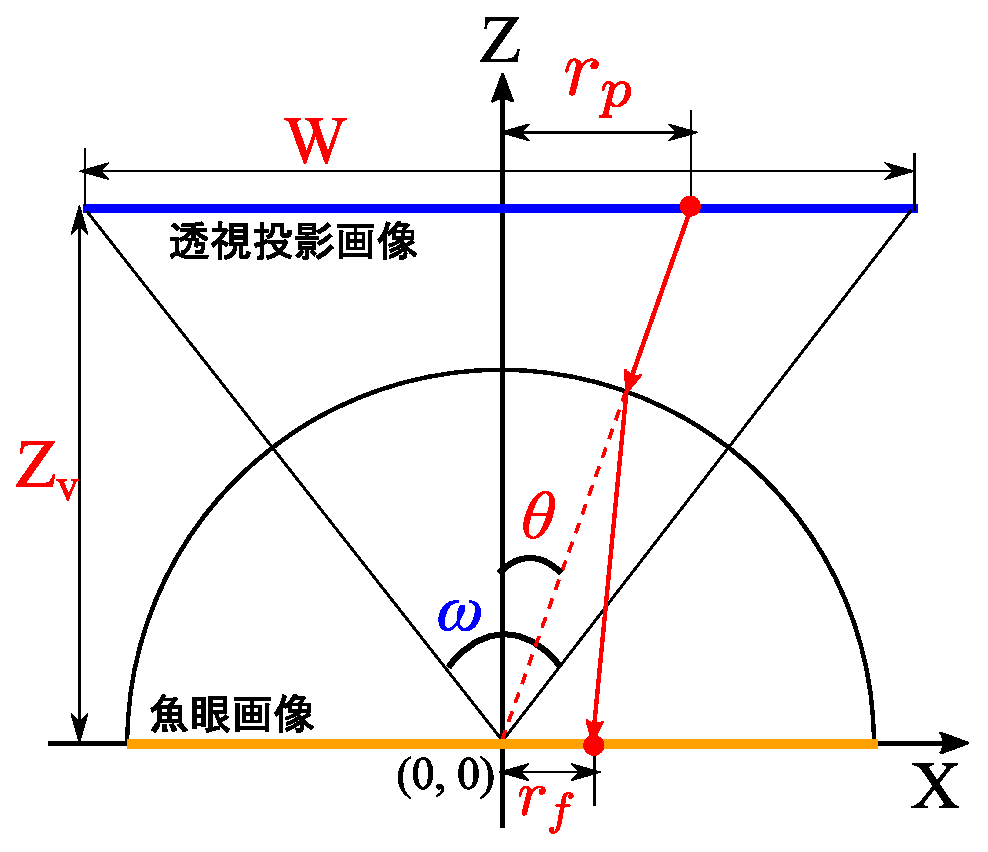
\includegraphics[width=7cm]{./chap3/eps/Fisheye2perspective.eps}
%\vspace{-0.5cm}
\caption{�������e�摜��̓_���狛�჌���Y�ւ̓��ˌ��̗l�q}
\label{fig:fisheye_ray}
\end{center}
\end{figure}

\begin{figure}[tb]
\begin{center}
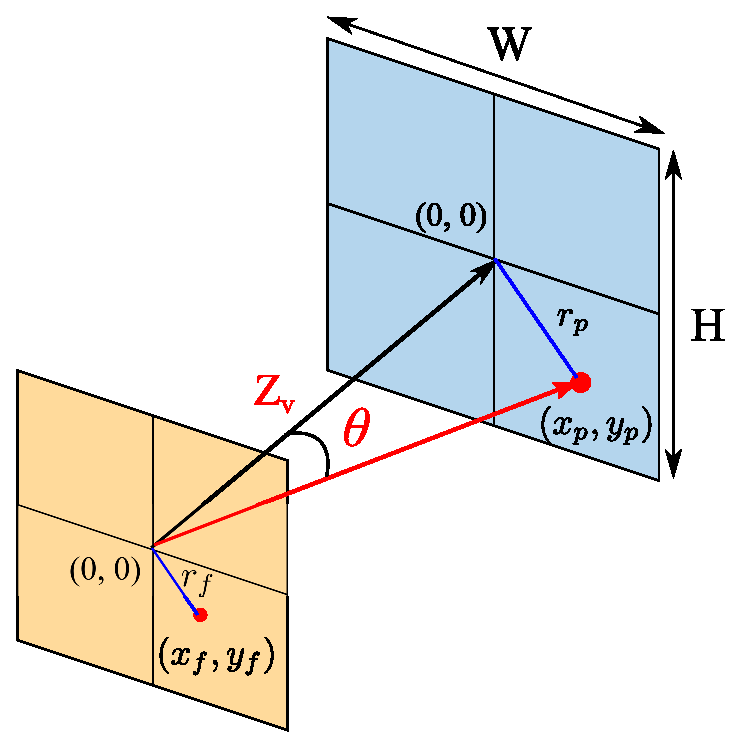
\includegraphics[width=7cm]{./chap3/eps/Fisheye2perspective2.eps}
\caption{�������e�摜��̓_�ƑΉ����鋛��摜��̓_�̊֌W}
\label{fig:hoseimen}
\end{center}
\end{figure}

�c�݂̕␳�ɍۂ��Ă܂��C����摜���瓧�����e�摜�ւƕϊ������p�͈͂��߂�D
�ʏ틛��摜�͉摜���S���痣���قǘc�݂��傫���␳������ɂȂ�D
�����Ōv�����x�̒ቺ������邽�߁C�{�����ł͉�p���ɂ߂đ傫���̈�͌v���͈͊O�Ƃ���D
�{�߂ł͔C�ӂ̉�p$\omega$ �͈̔͂ɂĕ␳�ʓW�J���s���Ƃ���D
���ɁC�␳�ʓW�J��̉摜�̍����C�������ꂼ��H�CW�Ƃ��C�}\ref{fig:fisheye_ray}�̂悤�ɏœ_����$Z_v$��ݒ肷��D
�������e�摜�ւ̕ϊ��́C�������e�摜��̍��W$(x_f, y_f)$�ɑΉ����鋛��摜��̓_$(x_p, y_p)$���Z�o���邱�Ƃōs���D
���჌���Y�ɂ��c�݂͉摜���S������˕����݂̂ł��邱�Ƃ���C����摜�̒��S����C�ӂ̓_$(x_f, y_f)$�܂ł̋�����$r_f$�C�������e�摜�̒��S����Ή�����_$(x_p, y_p)$�܂ł̋�����$r_p$�Ƃ���ƁC
�}\ref{fig:fisheye_ray}�C�}\ref{fig:hoseimen}���C$(x_f, y_f)$�C$(x_p, x_p)$�͎��̂悤�Ȋ֌W�����D

\begin{eqnarray}
\left[\begin{array}{cc}x_f\\y_f \end{array}\right] = \frac{r_f}{r_p} \left[\begin{array}{cc}x_p \\ y_p \end{array}\right]
\label{eq:XY}
\end{eqnarray}

����āC�������e�摜��̓_$(x_p, y_p)$�ɑΉ����鋛��摜��̓_$(x_f, y_f)$�����߂邽�߂ɂ�$r_f$�C$r_p$�̒l�����܂�Ηǂ��D
�����ŁC$r_p$�͐}\ref{fig:fisheye_ray}���C����(\ref{eq:R})�ɂ�苁�܂�D

\begin{eqnarray}
r_p = \sqrt{ x_p^2 + y_p^2}
\label{eq:R}
\end{eqnarray}

�܂��C$r_f$�͎�(\ref{eq:theta_r})���C$\theta$�̒l����܂�ΎZ�o�ł���D$\theta$�̒l�͎���(\ref{eq:theta})�C(\ref{eq:Zv})�ɂ��Z�o�����D
����������$r_f$�͎�(\ref{eq:r_p})�ɂ��C$x_p$�C$y_p$�C$Z_v$�̊֐��ŕ\�����D

\begin{eqnarray}
\theta = \cos^{-1} \frac{Zv}{\sqrt{ x_p^2 + y_p^2 + Z_v^2} }
\label{eq:theta}
\end{eqnarray}

\begin{eqnarray}
Z_v = \frac{W}{ 2\tan{\frac{\omega}{2}} }
\label{eq:Zv}
\end{eqnarray}

\begin{eqnarray}
r_f = j(x_p,y_p,Z_v)
\label{eq:r_p}
\end{eqnarray}

�ȏ�̊֌W���Ɋ�Â��C����摜���瓧�����e�摜�ւ̕ϊ����s���D










����摜�̘c�ݏ������s���O�̉摜�̗��}\ref{fig:before_expansion_120}�C���̉摜�𓧎����e�摜�ւƕϊ��������ʉ摜��}\ref{fig:after_expansion_120}�Ɏ����D
�}\ref{fig:before_expansion_120}���ɂ����ċ��჌���Y�ɂ��c��ł��������C�}\ref{fig:after_expansion_120}�̕␳�ʓW�J��̉摜���ł͒����ɂȂ��Ă��邱�Ƃ��m�F�ł���D


\begin{figure}[htb]
\begin{center}
\includegraphics[width=7cm]{./chap3/tmp/before_expansion.eps}
\caption{�␳�ʓW�J�O�̉摜�̗�i����J�����ł̎擾�摜�j}
\label{fig:before_expansion_120}
\end{center}
\end{figure}

\vspace{-0.5cm}

\begin{figure}[htb]
\begin{center}
\includegraphics[width=7cm]{./chap3/tmp/after_expansion.eps}
\caption{�␳�ʓW�J��̉摜�̗�}
\label{fig:after_expansion_120}
\end{center}
\end{figure}

\clearpage

%%%%%%%%%%%%%%%%%%%%%%%%%%%%%%%%%%%%%%%%%%%%%%%%%%%%%%%%%%%%%%%%%%%%%%%%%%%%%%%%%%%%%%%%%%%%%%%%%%%%%%%%%%%%%%%%%%%%%%%%%%%%%%%%%%%
\section{������}

�{�͂ł́C����J�����Ŏ擾�����摜�ɂ���ăI�[������3�����v�����s�����߂ɗp������W�n��K�v�ȃp�����[�^�C�摜�����ɂ‚��ďq�ׂ��D

�܂�\ref{sec:gaiyou2}�߂ł͖{�͂ōs���摜�����̊T�v�ɂ‚��ďq�ׁC\ref{sec:rectified}�߂Ŗ{�����ŋ���摜�΂𕽍s�X�e���I�y�A�Ƃ��Ĉ������߂ɒ�`������W�n�ɂ‚��ďq�ׂ��D

\ref{sec:fisheye_model}�߂ł́C��ʓI�ȃJ�����Ƌ���J�����̈Ⴂ�ɂ‚��ďq�ׂ���C���჌���Y�ɂ��c�݂̃��f���ɂ‚��Đ������C�{�����ŗp���鋛��J�����̃��f���ɂ‚��ďq�ׂ��D

\ref{sec:calibration}�߂Ŗ{�����ɂ�����摜�����ɕK�v�ȃp�����[�^�ƁC�����̐�����@�ɂ‚��ďq�ׂ��D

\ref{sec:translation}�߂ł́C���͉摜�΂𕽍s�X�e���I�摜�΂ւƕϊ�����摜������@�ɂ‚��ďq�ׂ��D

%���̍��W�n�ւ̉摜�̕ϊ����@�ɂ‚��ďq�ׂ�D�ϊ��ɂ�\ref{sec:calibration}�߂Ő��肵���p�����[�^��p����D

�Ō��\ref{sec:undistortion}�߂ł́C���͉摜���狛�჌���Y�ɂ��c�݂���菜���������e�摜�ւƕϊ������@�ɂ‚��ďq�ׂ��D

���͂ł́C���s������c�݂̏������ꂽ�I�[�����摜����͂Ƃ��C
�I�[������3�����v�����s��3�����Ž��������@�ɂ‚��ďq�ׂ�D
%�Ō��\ref{sec:backsubtraction}�߂ł́C�����_���o�̂��߂ɉ摜������I�[�����̈�𒊏o����w�i�����ɂ‚��ďq�ׂ�D
\clearpage



%%%%%%%%%%%%%%%%%%%%%%%%%%%%%%%%%%%%%%%%%%%%%%%%%%%%%%%%%%%%%%%%%%%%%%%%%%%%%%%%%%%%%%%%%%%%%%%%%%%%%%%%%%%%%%%%%%%%%%%%%%%%%%%%%%%
%%% Local Variables:
%%% mode: katex
%%% TeX-master: "../thesis"
%%% End:

\chapter{位置推定}
\thispagestyle{empty}
\label{chap4}
\minitoc

\newpage
%%%%%%%%%%%%%%%%%%%%%%%%%%%%%%%%%%%%%%%%%%%%%%%%%%%%%%%%%%%%%%%%%%%%%%%%%%%%%%%
%==============================================================================
% 4.1
%==============================================================================
\section{はじめに}

本章では,位置$\bm{P}$を推定する手法について述べる.

4.2節にて,手法の概要について述べる.

4.3節にて,特徴量の計算について述べる.

4.4節にて,$xy$座標の推定方法について述べる.

4.5節にて,$z$座標の推定方法について述べる.


\clearpage
%==============================================================================
% 4.2
%==============================================================================
\section{位置推定の概要}

位置推定では,各エッジ点とそれに対応する単位球面勾配ベクトル,姿勢$\bm{O}$,ラインマップからカメラの位置$\bm{P}$を推定する.
図\ref{fig:derotation}に示すように,ワールド座標系から姿勢$\bm{O}$の分ずれているカメラ座標系$x_{\rm{sph}}y_{\rm{sph}}z_{\rm{sph}}$を$\bm{O}^{-1}$回転させることでワールド座標系と向きが一致した状態に変換して位置を推定する.変換後のカメラ座標系を$x'_{\rm{sph}}y'_{\rm{sph}}z'_{\rm{sph}}$とする.
\\

\begin{figure}[b]
 \begin{center}
 \includegraphics[width=0.85\columnwidth]{./chap4/fig/derotation.png}
 \caption{ワールド座標系の向きと一致させるようなカメラ座標系の回転}
 \label{fig:derotation}
 \end{center}
\end{figure}

位置推定では,ワールド座標系における各軸方向の直線が球面に投影されたとき,それぞれの軸方向を法線ベクトルとする大円と交わる点の分布を特徴量とする.
この特徴量は,$y'_{\rm{sph}}z'_{\rm{sph}}$平面,$x'_{\rm{sph}}z'_{\rm{sph}}$平面,$x'_{\rm{sph}}y'_{\rm{sph}}$平面のそれぞれにおける単位円上の点の集合で表される.
例えば,図\ref{fig:feature_x}に示すように,青い実線で示す$x$軸方向に伸びる直線は青い破線で示す線のように球面に投影され,この破線と$x'_{\rm{sph}}$方向を法線ベクトルとする大円の交点は$y'_{\rm{sph}}z'_{\rm{sph}}$平面における単位円上に存在する.
すべての$x$軸方向の直線について同様に交点を計算すると,$y'_{\rm{sph}}z'_{\rm{sph}}$平面における単位円上の点の集合が得られる.
これと同様に,$y$軸方向に伸びる直線から$x'_{\rm{sph}}z'_{\rm{sph}}$平面における単位円上の点の集合が得られ(図\ref{fig:feature_y}),$z$軸方向に伸びる直線から$x'_{\rm{sph}}y'_{\rm{sph}}$平面における単位円上の点の集合が得られる(図\ref{fig:feature_z}).
これらをそれぞれ,$yz$特徴量,$xz$特徴量,$xy$特徴量と呼ぶ.
これらの特徴量は各カメラ位置において一意に定まるため,推定する画像の特徴量とラインマップから計算する各位置における特徴量を比較し,最も類似度の高い位置を探索することによりカメラの位置を推定することができる.
\\

\begin{figure}[tb]
 \begin{center}
 \includegraphics[width=0.85\columnwidth]{./chap4/fig/feature_x.png}
 \caption{$x$軸方向の直線から得られる$y'_{\rm{sph}}z'_{\rm{sph}}$平面における単位円上の点の集合}
 \label{fig:feature_x}
 \end{center}
\end{figure}

\begin{figure}[tb]
 \begin{center}
 \includegraphics[width=0.85\columnwidth]{./chap4/fig/feature_y.png}
 \caption{$y$軸方向の直線から得られる$x'_{\rm{sph}}z'_{\rm{sph}}$平面における単位円上の点の集合}
 \label{fig:feature_y}
 \end{center}
\end{figure}

\clearpage

\begin{figure}[tb]
 \begin{center}
 \includegraphics[width=0.85\columnwidth]{./chap4/fig/feature_z.png}
 \caption{$z$軸方向の直線から得られる$x'_{\rm{sph}}y'_{\rm{sph}}$平面における単位円上の点の集合}
 \label{fig:feature_z}
 \end{center}
\end{figure}


ここで,各軸方向の直線から得られる特徴量は,その軸方向のカメラ移動に依存せずに定まる.
つまり,$x$軸方向の直線から得られる$yz$特徴量はカメラの$yz$座標にのみにより定まり,$y$軸方向の直線から得られる$xz$特徴量はカメラの$xz$座標にのみにより定まり,$z$軸方向の直線から得られる$xy$特徴量はカメラの$xy$座標にのみにより定まる.
これを利用して,はじめに1つの特徴量を用いて2自由度の推定を行い,次に残りの特徴量から1つを選んで残りの1自由度の推定を行うことで,2自由度の推定と1自由度の推定に分離して行う.
本研究では,はじめに$xy$特徴量を用いた2次元の探索により$xy$座標を推定し,その後$xz$特徴量と推定された$x$座標を用いた1次元の探索により$z$座標を推定した.
\\

位置推定の流れを図\ref{fig:flow4}に示す.
まず,各エッジ点とそれに対応する単位球面勾配ベクトル,姿勢$\bm{O}$から推定する画像の特徴量を計算し,$xy$特徴量と$xz$特徴量を得る.
次に,得られた$xy$特徴量とラインマップから$xy$座標の推定を行い,推定値$x^*,\ y^*$を求める.
最後に,$xz$特徴量,推定値$x^*$,ラインマップから$z$座標の推定を行い,推定値$z^*$を求める.
以上の流れで,カメラの位置$\bm{P}$の推定値$\bm{P}^*=[x^*,\ y^*,\ z^*]^{\mathrm{T}}$を得る.


\begin{figure}[tb]
 \begin{center}
 \includegraphics[width=0.7\columnwidth]{./chap4/fig/flow4.png}
 \vspace{5mm}
 \caption{位置推定の流れ}
 \label{fig:flow4}
 \end{center}
\end{figure}

\clearpage
%==============================================================================
% 4.3
%==============================================================================
\section{特徴量の計算}

\subsection{エッジ点の分類}

エッジ点とそれに対応する単位球面勾配ベクトルの組から$xy$特徴及び$xz$特徴量を得るためには,それぞれの勾配ベクトルがどの軸方向の直線によるエッジ点から得られたものかによって分類する必要がある.
姿勢を推定したあと,3平面のうち最も近い平面からの距離が閾値以上の単位勾配ベクトルをoutlierとして除去する.
残った単位球面勾配ベクトルをそれぞれ最も近い平面ごとに分類することで,元の入力画像におけるエッジ点を,どの方向の直線に属するものかで3つのグループに分類する.
分類されたエッジ点の例を図\ref{fig:classified}に示す.
赤色のエッジ点が$x$軸方向の直線によるエッジ点,緑色のエッジ点が$y$軸方向の直線によるエッジ点,青色のエッジ点が$z$軸方向の直線によるエッジ点をそれぞれ表している.
\\

\begin{figure}[b]
 \begin{center}
 \includegraphics[width=0.7\columnwidth]{./chap4/fig/edge_inlier.png}
 \caption{分類されたエッジ点}
 \label{fig:classified}
 \end{center}
\end{figure}

\clearpage

\subsection{$xy$特徴量}

$xy$座標の推定に用いる$xy$特徴量には,$z$軸方向の直線が球上に投影される直線と全天球カメラの$x_{sph}y_{sph}$平面の交点の分布$(x_k,y_k)\ (k=1, 2,..., n)$を用いる.
特徴量の計算では,4.3.1項で分類したエッジ点のうち,$z$軸方向の直線に属するものを抽出して行う.
図\ref{fig:classified}に青色で示されたエッジ点がこれに該当する.
図\ref{fig:feature_xy}に示すように,抽出されたエッジ点座標を$(u_k, v_k)\ (k=1, 2,..., n)$,画像の幅を$w$とすると,交点$(x_k,y_k)$は以下の式によって求められる.

\begin{equation}
   \left(x_k,\ y_k\right) = \left(-\sin\frac{2\pi u_k}{w},\ -\cos\frac{2\pi u_k}{w}\right).
\end{equation}

\begin{figure}[b]
 \begin{center}
 \includegraphics[width=1.0\columnwidth]{./chap4/fig/feature_xy.png}
 \vspace{5mm}
 \caption{$xy$特徴量($x_{sph}y_{sph}$平面)の計算}
 \label{fig:feature_xy}
 \end{center}
\end{figure}

\clearpage
\subsection{$xz$特徴量}
$z$座標の推定に用いる$xz$特徴量には,$y$軸方向の直線が球上に投影される直線と全天球カメラの$x_{sph}z_{sph}$平面の交点の分布$(x_k,z_k)\ (k=1, 2,..., n)$を用いる.
まず,図\ref{fig:classified}に示すエッジ画像を$x$軸回りに-90 deg回転させることで,図\ref{fig:rotated_edge}のようなエッジ画像に変換する.
特徴量の計算では,このエッジ画像内のエッジ点のうち,$y$軸方向の直線に属するものを抽出して行う.
図\ref{fig:rotated_edge}に緑色で示されたエッジ点がこれに該当する.
図\ref{fig:feature_xz}に示すように,抽出されたエッジ点座標を$(u_k, v_k)\ (k=1, 2,..., n)$,画像の幅を$w$ pixelとすると,交点$(x_k,z_k)$は以下の式によって求められる.

\begin{equation}
   \left(x_k,\ z_k\right) = \left(-\sin\frac{2\pi u_k}{w},\ -\cos\frac{2\pi u_k}{w}\right).
\end{equation}

\begin{figure}[b]
 \begin{center}
 \includegraphics[width=0.7\columnwidth]{./chap4/fig/rotated_edge.png}
 \vspace{5mm}
 \caption{$x$軸回りに-90 deg回転させたエッジ画像}
 \label{fig:rotated_edge}
 \end{center}
\end{figure}


\begin{figure}[b]
 \begin{center}
 \includegraphics[width=1.0\columnwidth]{./chap4/fig/feature_xz.png}
 \vspace{5mm}
 \caption{$xz$特徴量($x_{sph}z_{sph}$平面)の計算}
 \label{fig:feature_xz}
 \end{center}
\end{figure}


\clearpage
%==============================================================================
% 4.4
%==============================================================================
\section{$xy$座標の推定}

$xy$座標の推定では,$z$座標を固定し,2次元の最適化によって推定する.
図\ref{fig:search_xy}に座標$(x,y)$における全天球カメラを上から見た図を示す.
緑色の点が上記の方法で求めた交点,赤色の点がラインマップから求めた,座標$(x,y)$から遮蔽されることなく見えるz軸方向の直線をそれぞれ表している.
画像から全ての直線を検出できるとは限らないため交点と直線の数は必ずしも一致せず,交点の数を$n$,直線の数を$m$とする.
各交点と直線の距離を,全天球カメラ座標系においてそれぞれが成す角によって定義し,すべての交点に対する最も近い直線までの距離の二乗和が最小となるような座標$(x,y)$を推定値とする.
交点の座標を$(x_k,y_k)\ (k=1, 2,..., n)$,ラインマップにおける$z$軸方向の直線の$xy$座標を$(x_l, y_l)\ (l=1, 2,...,m)$とすると,これらの距離$d_{k,l}$は,以下の式で得られる.
\begin{equation}
   d_{k,l} = \cos^{-1}\left(\frac{x_k(x_l-x)+y_k(y_l-y)}{\sqrt{(x_l-x)^2+(y_l-y)^2}}\right).
\end{equation}

$d_{k,l}\ (l=1,2,...,m)$のうち,最も小さいものを$d_k$とする.

\begin{equation}
   d_k = \min\left(d_{k,1},\ d_{k,2},\cdots,\ d_{k,m}\right).
\end{equation}

全ての交点における$d_k$の二乗和を最小とするようなパラメータ$(x^*,y^*)$が,$xy$座標の推定値である.
この非線形最適化を,Levenberg-Marquardt法を用いて解く.

\begin{equation}
(x^*,y^*)=\argmin_{x,y} \sum_{k=1}^nd_k^2.
\label{eq:optim2}
\end{equation}

\begin{figure}[b]
 \begin{center}
 \includegraphics[width=0.6\columnwidth]{./chap4/fig/search_xy.png}
 \caption{座標$(x,y)$における全天球カメラを$z$軸方向から見た図}
 \label{fig:search_xy}
 \end{center}
\end{figure}


\clearpage
%==============================================================================
% 4.4
%==============================================================================
\section{$z$座標の推定}

$z$座標の推定では,$y$座標と前節で推定した$x$座標を固定し,1次元の最適化によって推定する.
まず,$xy$座標の推定と同様に,各交点$(x_k,z_k)$と$y$軸方向の直線の$xz$座標$(x_l,z_l)\ (l=1,2,...,m)$に対して以下の式で距離を計算する.

\begin{equation}
   d_{k,l} = \cos^{-1}\left(\frac{x_k(x_l-x^*)+z_k(z_l-z)}{\sqrt{(x_z-x^*)^2+(z_l-z)^2}}\right).
\end{equation}

$d_{k,l}\ (l=1,2,...,m)$のうち,最も小さいものを$d_k$とする.

\begin{equation}
   d_k = \min\left(d_{k,1},\ d_{k,2},\cdots,\ d_{k,m}\right).
\end{equation}

全ての交点における$d_k$の二乗和を最小とするようなパラメータ$(z^*)$が,$z$座標の推定値である.
この非線形最適化を,Levenberg-Marquardt法を用いて解く.

\begin{equation}
(z^*)=\argmin_{z} \sum_{k=1}^nd_k^2.
\label{eq:optim2}
\end{equation}


\begin{figure}[b]
 \begin{center}
 \includegraphics[width=0.6\columnwidth]{./chap4/fig/search_xz.png}
 \caption{座標$(x,z)$における全天球カメラを$y$軸方向から見た図}
 \label{fig:search_xz}
 \end{center}
\end{figure}


\clearpage
%==============================================================================
% 4.5
%==============================================================================
\section{おわりに}

本章では,位置推定手法について説明した.

4.2節にて,位置推定の概要を述べた.

4.3節にて,特徴量の計算について述べた.

4.4節にて,$xy$座標の推定方法について述べた.

4.5節にて,$z$座標の推定方法について述べる.


次章では,提案手法の有効性を検証するために行った実験について述べる.

\clearpage
%%%%%%%%%%%%%%%%%%%%%%%%%%%%%%%%%%%%%%%%%%%%%%%%%%%%%%%%%%%%%%%%%%%%%%%%%%%%%%%%%
%%%%% Local Variables:
%%%%% mode: katex
%%%%% TeX-master: "../thesis"
%%%%% End:

\chapter{実験による提案手法の評価}
\label{chap:development}
\minitoc

\thispagestyle{empty}

\newpage
%%%%%%%%%%%%%%%%%%%%%%%%%%%%%%%%%%%%%%%%%%%%%%%%%%%%%%%%%%%%%%%%%%%%%%%%%%%%%%%%%%%%%%%%%%%%%%%%%%%%%%%%%%%%%%%%%%%%%%%%%%%%%%%%%%%
\section{はじめに}
\label{sec:intro_chap5}

本章では,理学療法士の技能を利用した,起立動作の支援機器の設計と開発,ならびに評価実験について述べる.

\ref{sec:design_chap5}節にて,支援機器の設計について述べる.

\ref{sec:development_chap5}節にて,支援機器の開発について述べる.

\ref{sec:experiment_chap5}節にて,支援機器の評価を行った実験について述べる.

\ref{sec:outro_chap5}節にて,本章のまとめを述べる.

\textcolor{red}{改ページする予定です.}
%\clearpage
%%%%%%%%%%%%%%%%%%%%%%%%%%%%%%%%%%%%%%%%%%%%%%%%%%%%%%%%%%%%%%%%%%%%%%%%%%%%%%%%%%%%%%%%%%%%%%%%%%%%%%%%%%%%%%%%%%%%%%%%%%%%%%%%%%%
\section{支援機器の設計}
\label{sec:design_chap5}

本節では,起立動作の支援機器の設計について述べる.\\

\textcolor{red}{改ページする予定です.}
%\clearpage
%%%%%%%%%%%%%%%%%%%%%%%%%%%%%%%%%%%%%%%%%%%%%%%%%%%%%%%%%%%%%%%%%%%%%%%%%%%%%%%%%%%%%%%%%%%%%%%%%%%%%%%%%%%%%%%%%%%%%%%%%%%%%%%%%%%
\section{支援機器の開発}
\label{sec:development_chap5}

本節では,起立動作の支援機器の開発について述べる.\\

\textcolor{red}{改ページする予定です.}
%\clearpage
%%%%%%%%%%%%%%%%%%%%%%%%%%%%%%%%%%%%%%%%%%%%%%%%%%%%%%%%%%%%%%%%%%%%%%%%%%%%%%%%%%%%%%%%%%%%%%%%%%%%%%%%%%%%%%%%%%%%%%%%%%%%%%%%%%%
\section{評価実験}
\label{sec:experiment_chap5}

本節では,開発した支援機器の評価を行うための実験について述べる.\\

\textcolor{red}{改ページする予定です.}
%\clearpage
%%%%%%%%%%%%%%%%%%%%%%%%%%%%%%%%%%%%%%%%%%%%%%%%%%%%%%%%%%%%%%%%%%%%%%%%%%%%%%%%%%%%%%%%%%%%%%%%%%%%%%%%%%%%%%%%%%%%%%%%%%%%%%%%%%%

\section{おわりに}
\label{sec:outro_chap5}

本章では,理学療法士の技能を利用した,起立動作の支援機器の設計と開発,ならびに評価実験について述べる.

\ref{sec:design_chap5}節にて,支援機器の設計について述べた.

\ref{sec:development_chap5}節にて,支援機器の開発について述べた.

\ref{sec:experiment_chap5}節にて,支援機器の評価を行った実験について述べた.\\

開発した支援機器により健常な高齢者の起立動作を支援することが可能であることを確認した.

\clearpage
%%%%%%%%%%%%%%%%%%%%%%%%%%%%%%%%%%%%%%%%%%%%%%%%%%%%%%%%%%%%%%%%%%%%%%%%%%%%%%%%%%%%%%%%%%%%%%%%%%%%%%%%%%%%%%%%%%%%%%%%%%%%%%%%%%%
%%% Local Variables:
%%% mode: katex
%%% TeX-master: "../thesis"
%%% End:

\chapter{結論}
\thispagestyle{empty}
\label{chap6}
\minitoc

\newpage
%%%%%%%%%%%%%%%%%%%%%%%%%%%%%%%%%%%%%%%%%%%%%%%%%%%%%%%%%%%%%%%%%%%%%%%%%%%%%%%
%==============================================================================
%まとめ
%==============================================================================
\section{結論}

本論文では,直線情報に基づく全天球カメラの高速な6自由度の位置姿勢推定手法を提案した.
\vspace{\baselineskip}

第1章にて,研究背景として位置姿勢推定における全天球カメラの優位性を示し,関連する従来研究では,大域的アプローチによる全天球カメラの6自由度の位置姿勢推定として,リアルタイムのアプリケーションに適用できるような高速な手法は提案されていないことを述べた.これに基づき本研究の目的を「全天球カメラを用いた大域的なアプローチによる高速な6自由度の位置姿勢推定」と設定した.
\vspace{\baselineskip}

第2章において,本研究のアプローチについて述べた.
本研究では,位置姿勢推定において位置の推定と姿勢の推定を分離して行い,初めに姿勢を推定してから位置を推定することを述べた.
姿勢推定は消失点を用いて行い,画像の勾配のみから推定することで高速化することを述べた.
位置推定は,$xy$座標の推定と$z$座標の推定を分離してそれぞれを高速に行うことを述べた.
\vspace{\baselineskip}

第3章では姿勢推定の提案手法について詳しく説明した.
姿勢推定は,単位球面勾配ベクトルの分布とマンハッタンワールドにおける互いに直交する3平面を比較することによって行うことを説明した.
単位球面勾配ベクトルの計算は,画像内の2次元の勾配ベクトルを変換することによって行い,歪みによる勾配の計算精度の低下を抑えるために,歪みの大きい領域における勾配の計算には,入力画像を球面に変換して3次元空間において回転させた画像を用いることを述べた.
\vspace{\baselineskip}

第4章では位置推定の提案手法について詳しく説明した.
$z$軸方向に伸びる直線が投影された球上の直線と全天球カメラの$xy$平面の交点の分布は,カメラの$xy$座標にのみ依存することから,これを利用してまず$xy$座標を推定することを述べた.
その後,$x$軸方向に伸びる直線が投影された球上の直線と全天球カメラの$yz$平面の交点の分布を利用して$z$座標を推定する手法を提案した.
\vspace{\baselineskip}

第5章では,提案手法の有効性を示すために行った実験について述べた.
シミュレーション環境および実環境において位置姿勢推定実験を行い,高速に推定可能であることを実証した.
一方で,推定精度に関しては改善の必要があることが確認された.
\vspace{\baselineskip}

本論文により,直線情報に基づく全天球カメラの高速な6自由度の位置姿勢推定手法が確立された.

\newpage
%==============================================================================
%今後の展望
%==============================================================================
\section{今後の展望}

本論文では,直線情報に基づく全天球カメラの高速な6自由度の位置姿勢推定手法を構築した.
位置姿勢を高速に推定することができたものの,推定精度に関しては課題が残る結果となった.
さらなる性能の向上のためには,直線以外の情報の活用が考えられる.
例えば,直線周辺のテクスチャ情報を利用することなどが例として挙げられる.
これにより,精度やロバスト性の向上が期待される.
\vspace{\baselineskip}

%また,本手法は大域的アプローチによって全天球カメラの位置姿勢推定を行った.環境全域からある程度の位置を推定することができれば全天球カメラ画像と3次元モデルの直線の対応を推定することができる.直線の対応を推定できれば,直線の対応を用いて位置姿勢を推定することでより高精度に位置姿勢推定が可能となる.
%\vspace{\baselineskip}

また,本手法で使用した変数や閾値の中には試行錯誤的に定められたものが数点存在する.
環境によっては,これらのパラメータが精度に影響を与えることも考えられる.
特に,エッジ検出のパラメータは直線検出の精度に大きな影響を与える可能性があり,環境によって適切に定める必要がある.
従って,これらのパラメータを適切に決定する手法の構築は本手法の実用化において必要な課題である.
\vspace{\baselineskip}

%また,本手法では屋内環境に着目した手法を提案したが,様々な用途に対応するためには屋外環境にも適用可能な手法の構築が必要となる.
%屋外環境では,日照条件の違いによる照明の変化や車などの移動物体など,屋内環境にはない課題が考えられる.
%これらの課題を克服するために,屋外環境に対応可能なディスクリプタの構築が必要となる.
%\vspace{\baselineskip}

このような課題を解決することで,本提案手法は全天球カメラの位置姿勢推定を行う際の一般的枠組みとして幅広く応用可能になることが期待できる.


\newpage

%%%%%%%%%%%%%%%%%%%%%%%%%%%%%%%%%%%%%%%%%%%%%%%%%%%%%%%%%%%%%%%%%%%%%%%%%%%%%%%%
%%%% Local Variables:
%%%% mode: katex
%%%% TeX-master: "../thesis"
%%%% End:

}

%
% ☆☆☆☆☆☆☆☆☆☆☆☆☆☆☆☆☆☆☆☆☆☆☆☆☆☆☆☆☆☆☆☆ %
%                                                    謝辞
% ☆☆☆☆☆☆☆☆☆☆☆☆☆☆☆☆☆☆☆☆☆☆☆☆☆☆☆☆☆☆☆☆ %
\addcontentsline{toc}{chapter}{謝辞}
\chapter*{謝辞}
\thispagestyle{empty}
\markboth{謝辞}{}
\label{thankyou}
%\def\thepage{}

\newpage

本論文の締めくくりに,本研究を進めるにあたってご指導,ご協力をいただいた全ての方々に,
深く感謝申し上げます.
\\

本研究の指導教員である東京大学大学院 工学系研究科 精密工学専攻准教授 山下 淳先生には,
お忙しい中親身に,そして熱心にご指導いただきました.
研究のストーリーの組み立て方から論文や発表における効果的な表現の仕方まで,研究活動におけるあらゆることを学ばせていただきました.
また,非常に多くの学生のご指導をされていたのにも関わらず,一切手を抜かずに全ての学生に対して親身になってご指導される姿に感銘を受けました.
山下先生に教わったことを胸に刻み,今後の人生を歩んでいきたいと思っています.
誠にありがとうございました.
\\

本研究の副査を引き受けていただいた東京大学大学院 工学系研究科 人工物工学研究センター准教授 大竹 豊先生には,ご多忙の中,研究内容に対してたくさんの有意義なご指摘,ご助言をいただきました.
大竹先生からいただいたご意見によって,自分の研究を新たな視点から見つめなおすことができ,非常に勉強になりました.
ここに深く感謝申し上げます.
誠にありがとうございました.
\\

東京大学大学院 工学系研究科 精密工学専攻教授 淺間 一先生には,
ミーティングや発表練習の場で,論理的な考え方や伝わりやすいプレゼンテーションの仕方について丁寧にご指導いただきました.
第一線でご活躍なさっている淺間先生に指導していただいたことは大きな刺激となり,今後の人生においても有意義な経験となりました.
ここに深く感謝申し上げます.
ありがとうございました.
\\

千葉工業大学 先進工学部 未来ロボティクス学科准教授 藤井 浩光先生には,
本研究を進めるにあたってあらゆる場面でお世話になりました.
研究の過程でトラブルが生じた際に親身になって解決の手助けをしていただいたり,論文における文章の論理的なつながりを細かくチェックしていただいたりしたことは,大きな助けとなりました.
深く感謝申し上げます.
ありがとうございました.
\\

中央大学 理工学部 精密機械工学科助教 池 勇勳先生には,
研究内容に関するご意見やご助言,そして論文のチェックなどで研究を支えていただきました.
また研究以外においても,一緒に食事に行ったりと気さくに接していただき,楽しく過ごすことができました.
深く感謝申し上げます.
ありがとうございました.
\\

東京大学大学院 工学系研究科 精密工学専攻外国人特別研究員 Sarthak Pathak博士には,
本研究を一番近くで支えていただきました.
不自由なく研究を行う環境を整えていただくところから,研究内容についての議論,プログラムの実装や実験の手助け,そして論文やプレゼン資料のチェックまで,研究活動のあらゆる場面で支えていただき,頼りになる存在でした.
また研究以外においても,皆で交流する機会を積極的に設けてくださり,全天球グループの親睦を深めることができました.
深く感謝いたします.
ありがとうございました.
\\

東京大学大学院 工学系研究科 総合研究機構特任助教 濱崎 峻資博士には,
本論文のチェックをしていただきました.
様々な角度からのご指摘は非常に参考になり,より良い論文に仕上げることができました.
深く感謝いたします.
\\

研究室の先輩である樋口 寛氏には,
オブザーバとして参加していただいていたミーティングで,大変有意義なアドバイスをいただきました.
樋口さんの鋭いご意見によって,本研究をより良いものにすることができました.
誠にありがとうございました.
\\

研究室の同期である川田 桃子氏,山内 統広氏,金 ダベ氏,呉 家旭氏,長野 樹氏,湊 真司氏,尹 ソンミン氏とは,
研究生活だけでなく私生活においても多くの時間を共に過ごし,お互い切磋琢磨しながら充実した日々を過ごすことができました.
特に,同じ研究グループの金君には,研究の手助けもしていただきました.
ありがとうございました.
\\

その他研究室の皆様には,日頃から大変お世話になりました.
スタッフの皆様には,研究生活における様々な面においてサポートをしていただきました.
秘書の皆様には,物品の購入や出張時の手続きなどの事務作業を行っていただき,研究に専念して日々を過ごすことができました.お菓子などの差し入れも大変ありがたかったです.
学生の皆様には,研究に対しそれぞれ真摯にひたむきに取り組む姿から大変良い刺激を受けました.
日々の生活やイベント等で皆様と楽しく過ごせたことも大切な思い出です.
ありがとうございました.
\\

崔氏,青野氏,後藤氏をはじめとする友人の皆様には,日頃から励ましていただいたり,息抜きに付き合っていただいたりと,大きな支えとなりました.
ありがとうございました.
\\

最後に,これまで私を支えてくれた家族に深く感謝の意を表します.本当にありがとうございました.
%\\

\begin{flushright}
2020年 2月 野田 純平
\end{flushright}


\newpage
%%%%%%%%%%%%%%%%%%%%%%%%%%%%%%%%%%%%%%%%%%%%%%%%%%%%%%%%%%%%%%%%%%%%%%%%%%%%%%%

%%%%%%%%%%%%%%%%%%%%%%%%%%%%%%%%%%%%%%%%%%%%%%%%%%%%%%%%%%%%%%%%%%%%%%%%%%%%%%%
%%% Local Variables:
%%% mode: katex
%%% TeX-master: "../thesis"
%%% End:

\cleardoublepage

% ☆☆☆☆☆☆☆☆☆☆☆☆☆☆☆☆☆☆☆☆☆☆☆☆☆☆☆☆☆☆☆☆ %
%                                                 参考文献
% ☆☆☆☆☆☆☆☆☆☆☆☆☆☆☆☆☆☆☆☆☆☆☆☆☆☆☆☆☆☆☆☆ %
%\bibliographystyle{junsrt}
%\bibliography{ref}

\addcontentsline{toc}{chapter}{参考文献}
\chapter*{参考文献}
\label{ref}
%\addcontentsline{toc}{chapter}{参考文献}
\lhead[参考文献]{}
%\renewcommand{\refname}{引用文献}
\thispagestyle{empty}


\newpage
%%%%%%%%%%%%%%%%%%%%%%%%%%%%%%%%%%%%%%%%%%%%%%%%%%%%%%%%%%%%%%%%%%%%%%%%%%%%%%%
\subsection*{\textmc{<和文文献>}}

\begin{mythebibliography}{99}

\bibitem[厚生労働省 2014]{厚労省2014}
\leavevmode \\
厚生労働省:
\newblock ``平成26年 患者調査の概況'',
\newblock 2014.
\\

\bibitem[厚生労働省 2016]{厚労省2016}
\leavevmode \\
厚生労働省:
\newblock ``平成28年 国民生活基礎調査の概況'',
\newblock 2016.
\\

\bibitem[脳卒中治療ガイドライン 2009]{脳卒中2009}
\leavevmode \\
日本脳卒中学会 脳卒中合同ガイドライン委員会 編:
\newblock ``脳卒中治療ガイドライン2009'',
\newblock http://www.jsts.gr.jp/main08a.html, 2009, 閲覧日2018.12.13.
\\

\bibitem[道免 2015]{道免2015}
\leavevmode \\
道免 和久 編:
\newblock ``ニューロリハビリテーション'',
\newblock 医学書院, 2015.
\\

\bibitem[有末 2015]{有末2015}
\leavevmode \\
有末 伊織, 田中 直次郎, 藤井 靖晃, 藤高 裕太, 中本 舞, 松本 強, 丸田 佳克, 福江 亮, 松下 信郎, 山岡 まこと, 橋本 陽平, 園田 泰, 霜山 香織, 福間 美佑貴, 岡本 隆嗣:
\newblock ``歩行アシストロボットを用いた 回復期脳卒中患者に対する歩行練習の影響 ─歩行速度による違い─'',
\newblock 理学療法科学, Vol.~20, No.~1, pp.~119--123, 2015.
\\

\bibitem[渡邊 2016]{渡邊2016}
\leavevmode \\
渡邊 亜紀, 川井 康平, 佐藤 浩二, 宮崎 吉孝, 伊藤 寿弘, 森 照明:
\newblock ``HONDA歩行アシストの継続使用による脳卒中片麻痺者の歩行変化'',
\newblock 理学療法学, Vol.~43, No.~4, pp.~337--341, 2016.
\\

\bibitem[長田 2012]{長田2012}
\leavevmode \\
長田 悠路, 山本 澄子, 渕 雅子:
\newblock ``脳卒中片麻痺患者の起立動作における運動学的・運動力学的評価指標'',
\newblock 理学療法学, Vol.~39, No.~3, pp.~149--158, 2012.
\\

\bibitem[津坂 2017]{津坂2017}
\leavevmode \\
津坂 優子, F. Dallalibera, 岡崎 安直, 山本 正樹, 横小路 泰義:
\newblock ``理学療法士のスキルを活かした自立支援型起立アシストロボットの開発'',
\newblock 日本機械学会論文集, Vol.~83, No.~852, pp.~1--14, 2017.
\\

%\bibitem[橋本 2001]{橋本2001}
%\leavevmode \\
%橋本 秀紀, 秋山 尊志:
%\newblock ``空間知能化―インテリジェント・スペースの提案'',
%\newblock 生産研究, Vol.~53, No.~5, pp.~257--267, 2001.
%\\

%\end{mythebibliography}
\newpage
%%%%%%%%%%%%%%%%%%%%%%%%%%%%%%%%%%%%%%%%%%%%%%%%%%%%%%%%%%%%%%%%%%%%%%%%%%%%%%%
\subsection*{\textmc{\hspace{-1zw}<英文文献>}}

\bibitem[Guralnik 1994]{Guralnik1994}
\leavevmode \\
J. M. Guralnik, E. M. Simonsick, L. Ferrucci, R. J. Glynn, L. F. Berkman, D. G. Blazer, P. A. Scherr and R. B. Wallace:
\newblock ``A Short Physical Performance Battery Assessing Lower Extremity Function: Association with Self-Reported Disability and Prediction of Mortality and Nursing Home Admission'',
\newblock {\itshape Journals of Gerontology}, Vol.~49, No.~2, pp.~85--94, 1994. 
\\

\bibitem[Fisher 2011]{Fisher2011}
\leavevmode \\
S. Fisher, L. Lucas and T. A. Thrasher:
\newblock ``Robot-Assisted Gait Training for Patients with Hemiparesis Due to Stroke'',
\newblock {\itshape Topics in Stroke Rehabilitation}, Vol.~18, No.~3, 2011. 
\\

\bibitem[Srivastava 2016]{Srivastava2016}
\leavevmode \\
S. Srivastava, P. C. Kao, D. S. Reisman, J. P. Scholz and S. K. Agrawal:
\newblock ``Robotic assist-as-needed as an alternative to therapist-assisted gait rehabilitation'',
\newblock {\itshape International journal of physical medicine \& rehabilitation}, Vol.~4, No.~5, pp.~370, 2016. 
\\

\bibitem[Chou 2003]{Chou2003}
\leavevmode \\
S. W. Chou, A. M. K. Wong, C. P. Leong, W. S. Hong, F. K. Tang and T. H. Lin:
\newblock ``Postural control during sit-to stand and gait in stroke patients'',
\newblock {\itshape American Journal of Physical Medicine and Rehabilitation}, vol.~82, no.~1, pp.~42--47, 2003.
\\

\bibitem[Tsukahara 2010]{Tsukahara2010}
\leavevmode \\
A. Tsukahara, R. Kawanishi, Y. Hasegawa and Y. Sankai:
\newblock ``Sit-to-stand and stand-to-sit transfer support for complete paraplegic patients with robot suit HAL'',
\newblock {\itshape Advanced Robotics}, Vol.~24, No.~11, pp.~1615--1638, 2010. 
\\

\bibitem[Shiraishi 2016]{Shiraishi2016}
\leavevmode \\
R. Shiraishi, H. Kawamoto and Y. Sankai:
\newblock ``Development of sit-to-stand and stand-to-sit training system for hemiplegie patients'',
\newblock {\itshape Proceedings of the Annual International Conference of the IEEE Engineering in Medicine and Biology Society}, pp.~4567--4572, 2016. 
\\

\bibitem[Mourey 2000]{Mourey2000}
F. Mourey, A. Grishin, P. D'Athis, T. Pozzo and P. Stapley:
\newblock ``Standing up from a chair as a dynamic equilibrium task: a comparison between young and elderly subjects'',
\newblock {\itshape The journals of gerontology. Series A, Biological sciences and medical sciences}, vol.~55, no.~9, pp.~B425--B431, 2000.
\\

\bibitem[Yang 2017]{Yang2017}
N. Yang, Q. An, H. Yamakawa, Y. Tamura, A. Yamashita, K. Takahashi, M. Kinomoto, H. Yamasaki, M. Itkonen, F. S. Alnajjar, S. Shimoda, H. Asama, N. Hattori and I. Miyai:
\newblock ``Clarification of muscle synergy structure during standing-up motion of healthy young, elderly and post-stroke patients'',
\newblock {\itshape 2017 International Conference on Rehabilitation Robotics (ICORR)}, pp.~19--24, 2017.
\\

\bibitem[Silva 2013]{Silva2013}
A. Silva, A. S. P. Sousa, R. Pinheiro, J. Ferraz, J. M. R. S. Tavares, R. Santos and F. Sousa:
\newblock ``Activation timing of soleus and tibialis anterior muscles during sit-to-stand and stand-to-sit in post-stroke vs. healthy subjects'',
\newblock {\itshape Somatosensory and Motor Research}, vol.~30, No.~1,  pp.~48--55, 2013.
\\

%\bibitem[Huges 1994]{Hughes1994}
%\leavevmode \\
%M. A. Hughes, D. K. Weiner, M. L. Schenkman, R. M. Long and S. A. Studenski:
%\newblock ``Chair rise strategies in the elderly'',
%\newblock {\itshape Clinical Biomechanics}, vol.~9, no.~3, pp.~187--192, 1994.

\bibitem[Gross 1998]{Gross1998}
\leavevmode \\
M. M. Gross, P. J. Stevenson, S. L. Charette, G. Pyka and R. Marcus:
\newblock ``Effect of muscle strength and movement speed on the biomechanics of rising from a chair in healthy elderly and young women'',
\newblock {\itshape  Gait and Posture}, vol.~8, no.~3, pp.~175--185, 1998.
\\

%\bibitem[Brunt 2002]{Brunt2002}
%D. Brunt, B. Greenberg, S. Wankadia, M. A. Trimble and O. Shechtman:
%\newblock ``The effect of foot placement on sit to stand in healthy young subjects and patients with hemiplegia'',
%\newblock {\itshape Archives of Physical Medicine and Rehabilitation}, vol.~83, no.~7, pp.~924--929, 2002.
%\\

\bibitem[Chugo 2007]{Chugo2007}
D. Chugo, K. Kawabata, H. Okamoto, H. Kaetsu, H. Asama, N. Miyake, K. Kosuge:
\newblock ``Force assistance system for standing up motion'',
\newblock {\itshape Industrial Robot: An International Journal}, Vol.~34, No.~2, pp.~128--134, 2007.
\\

\bibitem[Tsusaka 2015]{Tsusaka2015}
Y. Tsusaka, Y. Okazaki, Y. Fudaba, R. Futakuchi, M. Yamamoto, N. Shikata, M. Terashima, T. Funatani, H. Shima:
\newblock ``Development of standing-up motion assist robot to realize physiotherapist skill for muscle strength maintenance'',
\newblock {\itshape Proceedings - IEEE International Workshop on Robot and Human Interactive Communication}, pp.~140--145, 2015.
\\

\clearpage

\end{mythebibliography}

%%%%%%%%%%%%%%%%%%%%%%%%%%%%%%%%%%%%%%%%%%%%%%%%%%%%%%%%

\cleardoublepage

% ☆☆☆☆☆☆☆☆☆☆☆☆☆☆☆☆☆☆☆☆☆☆☆☆☆☆☆☆☆☆☆☆ %
%                                                 研究業績
% ☆☆☆☆☆☆☆☆☆☆☆☆☆☆☆☆☆☆☆☆☆☆☆☆☆☆☆☆☆☆☆☆ %
\addcontentsline{toc}{chapter}{研究業績}
\chapter*{研究業績}
\thispagestyle{empty}
\lhead[研究業績]{}
\markboth{研究業績}{}
\label{achive}
%\def\thepage{}

\newpage
%==============================================================================
%本論文と関係がある業績
%==============================================================================
\section*{学術論文}
%\subsection*{学術論文}
%\begin{enumerate}[{[}1{]}]
\mbox{}
\begin{enumerate}
\item
\textbf{野田 純平}, Sarthak Pathak, 藤井 浩光, 山下 淳, 淺間 一: ``計測点の信頼度を考慮した全天球ステレオカメラの運動推定”,精密工学会誌, Vol.~85, No.~6, pp.~568--576, 2019.
\\
\item
\textbf{Jumpei Noda}, Sarthak Pathak, Yonghoon Ji, Hiromitsu Fujii, Atsushi Yamashita, Hajime Asama: ``Fast Rotation Estimation of Spherical Camera in Man-made Environments Based Only on Image Gradients”, IEEE Signal Processing Letters (to be submitted).
\end{enumerate}

%==============================================================================
%査読有り国内論文投稿
%==============================================================================
%\section*{査読有り学術論文}
%\begin{enumerate}[{[}1{]}]
%\mbox{}
%\begin{enumerate}
%\item 
%\textbf{柴田 彬}, 藤井 浩光, 山下 淳, 淺間 一: “単眼カメラと透明平板による屈折を利用したスケール復元が可能なStructure from Motion”, 精密工学会誌論文集(審査中).\\
%\end{enumerate}

%==============================================================================
%査読有り国際会議
%==============================================================================
%\section*{査読有り国際会議}
%%\begin{enumerate}[{[}1{]}]
%\mbox{}
%
%\begin{enumerate}
%
%\item
%\textbf{Yukari Okumura}, Hiromitsu~Fujii, Atsushi~Yamashita and Hajime~Asama: ``Global Optimization with Viewpoint Selection for Scale-reconstructible Structure from Motion Using Refraction", Proceedings of the International Workshop on Advanced Image Technology 2017 (IWAIT2017), Malaysia, Penang, January 2017. 
 


%\item 
%\textbf{Akira Shibata}, Hiromitsu~Fujii, Atsushi~Yamashita and Hajime~Asama: “Absolute Scale Structure from Motion Using a Refractive Plate”, the 2015 IEEE/SICE International Symposium on System Integration (SII2015), pp.~540--545, Nagoya, Japan, December 2015.
%\\

%\end{enumerate}

%==============================================================================
%査読有り国内会議
%==============================================================================
%\section*{査読有り国内会議}
%\begin{enumerate}[{[}1{]}]
%\mbox{}
%\begin{enumerate}
%\item 
%\textbf{柴田 彬}, 藤井 浩光, 山下 淳, 淺間 一: “屈折を利用した単眼カメラによる
%スケール復元が可能なStructure from Motion”, 第20回ロボティクスシンポジア講演予稿集, pp.~25--30, 軽井沢, March 2015.\\
%\\
%\end{enumerate}
%\clearpage

\mbox{}
%==============================================================================
%査読無し国内会議
%==============================================================================
\section*{査読無し国内会議}
%\begin{enumerate}[{[}1{]}]
\mbox{}

\begin{enumerate}
\item
\textbf{野田 純平}, Sarthak Pathak, 藤井 浩光, 山下 淳, 淺間 一: ``計測点の信頼度を考慮した全天球ステレオカメラによる運動推定”,第18回計測自動制御学会システムインテグレーション部門講演会予稿集, pp.~608--612, 2017.
\\
\end{enumerate}



%\section*{学術受賞}
%%\begin{enumerate}[{[}1{]}]
%\mbox{}
%\begin{enumerate}
%\item 
%\textbf{Akira Shibata}, Hiromitsu~Fujii, Atsushi~Yamashita and Hajime~Asama: “Scale-reconstructable Structure from Motion Using Refraction with a Single Camera”, the 2015 IEEE International Conference on Robotics and Automation (ICRA2015),
%\textbf{IEEE Robotics and Automation Society (RAS) Japan Chapter Young Award}, Seattle, USA, May 2015.
%\end{enumerate}
%%%%%%%%%%%%%%%%%%%%%%%%%%%%%%%%%%%%%%%%%%%%%%%%%%%%%%%%%%%%%%%%%%%%%%%%%%%%%%%

%%%%%%%%%%%%%%%%%%%%%%%%%%%%%%%%%%%%%%%%%%%%%%%%%%%%%%%%%%%%%%%%%%%%%%%%%%%%%%%
%%% Local Variables:
%%% mode: katex
%%% TeX-master: "../thesis"
%%% End:

\cleardoublepage

% ☆☆☆☆☆☆☆☆☆☆☆☆☆☆☆☆☆☆☆☆☆☆☆☆☆☆☆☆☆☆☆☆ %
%                                                    付録
% ☆☆☆☆☆☆☆☆☆☆☆☆☆☆☆☆☆☆☆☆☆☆☆☆☆☆☆☆☆☆☆☆ %
%\appendix
%\setcounter{chapter}{1}

%\newcommand{\furoku}[1]{\chapter{\thechapter\hspace{1.6zw}#1}}
%\newcommand{\furoku}[1]{\chapter{\thechapter \\ #1}}

%\chapter{従来のStructure from Motion手法}
\lhead[付録A 従来のStructure from Motion手法]{}
\setcounter{page}{1}
\renewcommand{\thepage}{A--\arabic{page}}

\thispagestyle{empty}

\newpage
%%%%%%%%%%%%%%%%%%%%%%%%%%%%%%%%%%%%%%%%%%%%%%%%%%%%%%%%%%%%%%%%%%%%%%%%%%%%%%%
\section{はじめに}

本付録では,屈折を用いていない従来のStructure from Motionについて述べる.

A.2節にて,従来のStructure from Motionの概要について述べる.

A.3節にて,従来のStructure from Motionの理論の詳細について述べる.



\newpage

\section{従来のStructure from Motionの概要}

ここでは,屈折を用いていない従来のStructure from Motionの概要を述べる.
本付録では,従来のStructure from Motionの計算方法の1つである8点法について述べる.
8点法はLonguet-HigginsやHartleyらによって開発された,Structure from Motionの計算方法の中で最も基本的な手法である\cite{Longuet-Higgins1981}\cite{Hartley2004}.

従来の8点法の流れを\mbox{図\ref{}に示す.}


\newpage

%%%%%%%%%%%%%%%%%%%%%%%%%%%%%%%%%%%%%%%%%%%%%%%%%%%%%%%%%%%%%%%%%%%%%%%%%%%%%%%
%%% Local Variables:
%%% mode: katex
%%% TeX-master: "../thesis"
%%% End:


%\chapter{水中Structure from Motionの研究との違いについて}
\lhead[付録B 水中Structure from Motionの研究との違いについて]{}
\setcounter{page}{1}
\renewcommand{\thepage}{B--\arabic{page}}

\thispagestyle{empty}

\newpage
%%%%%%%%%%%%%%%%%%%%%%%%%%%%%%%%%%%%%%%%%%%%%%%%%%%%%%%%%%%%%%%%%%%%%%%%%%%%%%%
\section{はじめに}




\newpage

\section{水中Structure from Motionの研究との違いについて}


\newpage


%%%%%%%%%%%%%%%%%%%%%%%%%%%%%%%%%%%%%%%%%%%%%%%%%%%%%%%%%%%%%%%%%%%%%%%%%%%%%%%
%%% Local Variables:
%%% mode: katex
%%% TeX-master: "../thesis"
%%% End:

%\cleardoublepage

%
% 論文の最後
\end{document}